\documentclass[11pt]{article}
\usepackage[a4paper,margin=1in]{geometry}
\usepackage[T1]{fontenc}\usepackage[utf8]{inputenc}
\usepackage{amsmath,amssymb,amsthm} % maths + theorems
\usepackage{graphicx} % images
\usepackage[table,dvipsnames]{xcolor} % colour + coloured tables
\usepackage{multirow,array,booktabs} % strong tables
\usepackage{subcaption,wrapfig} % subfigures, wrapped figures
\usepackage{enumitem} % custom list labels
\usepackage{listings} % code
\usepackage{authblk} % numbered author affiliations
\usepackage{hyperref} % LOAD LAST: links + clickable TOC
\usepackage{lipsum}


\title{FU}

\begin{document}


\begin{figure}
    \centering
    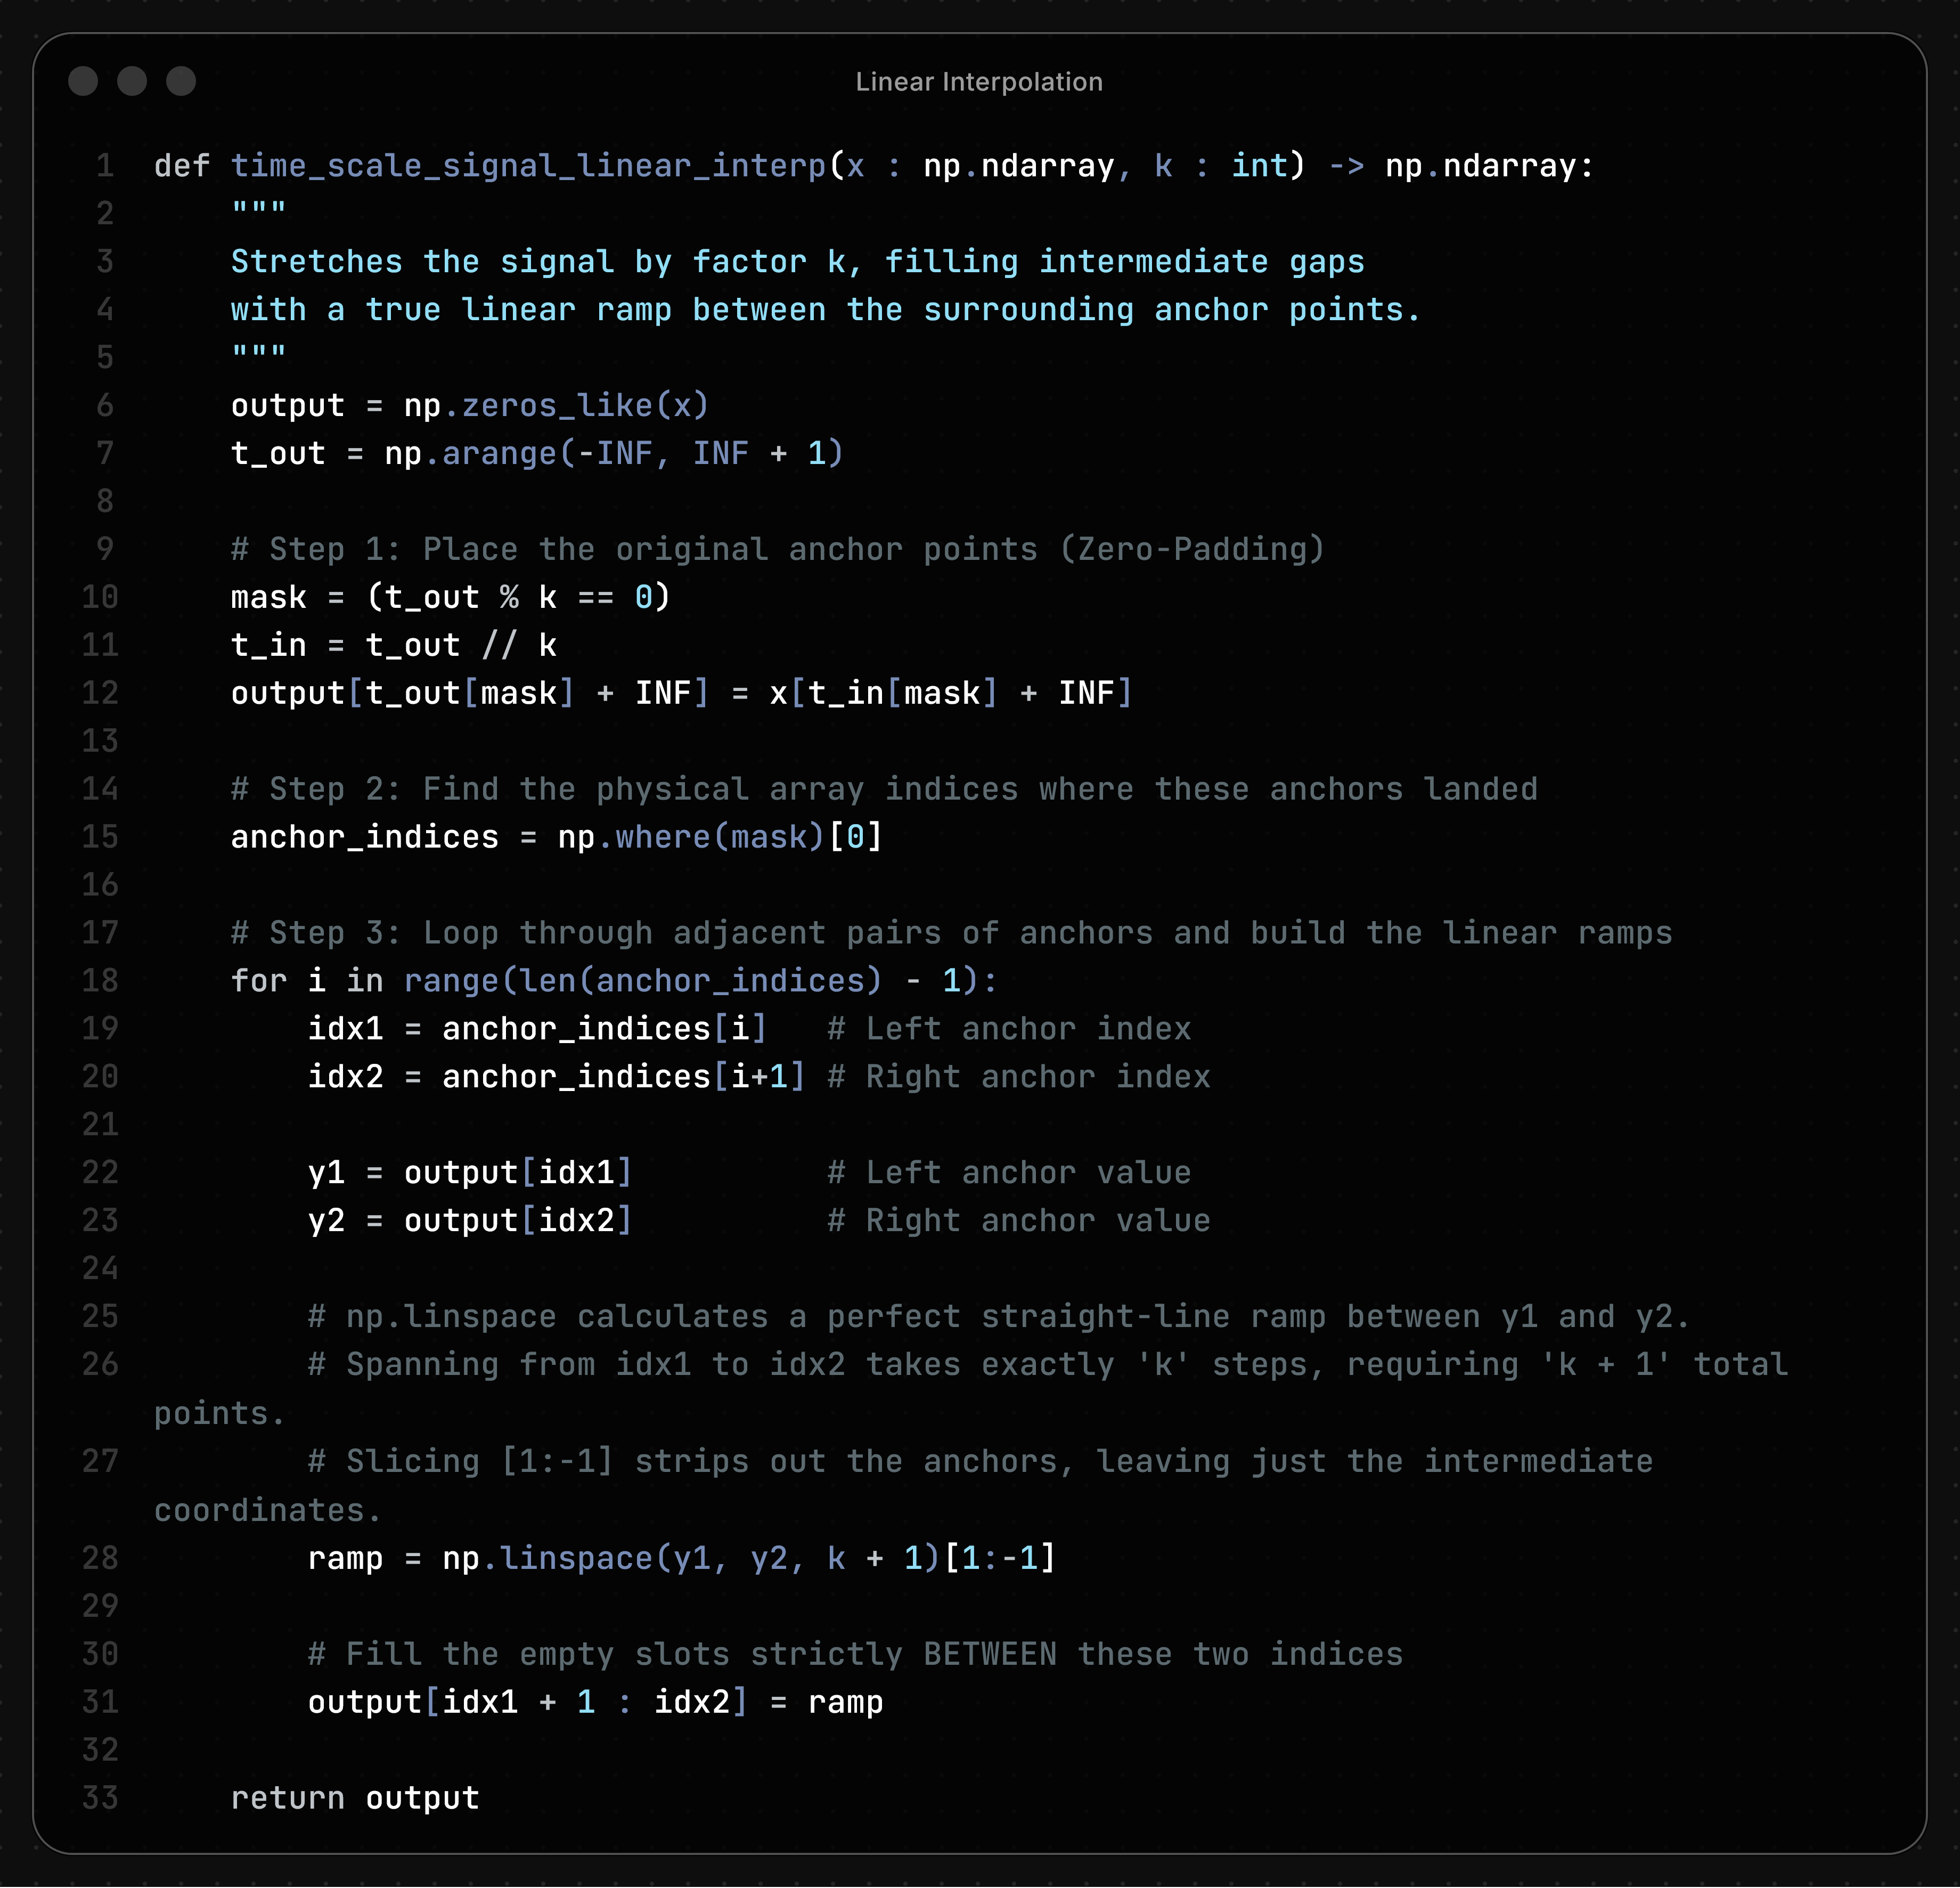
\includegraphics[width=0.45\textwidth]{li.png}

    \caption{The reference waveform}
    \label{the-ref-wf}

\end{figure}

\begin{figure}
    \centering
    \begin{minipage}{0.45\textwidth}
    \centering
    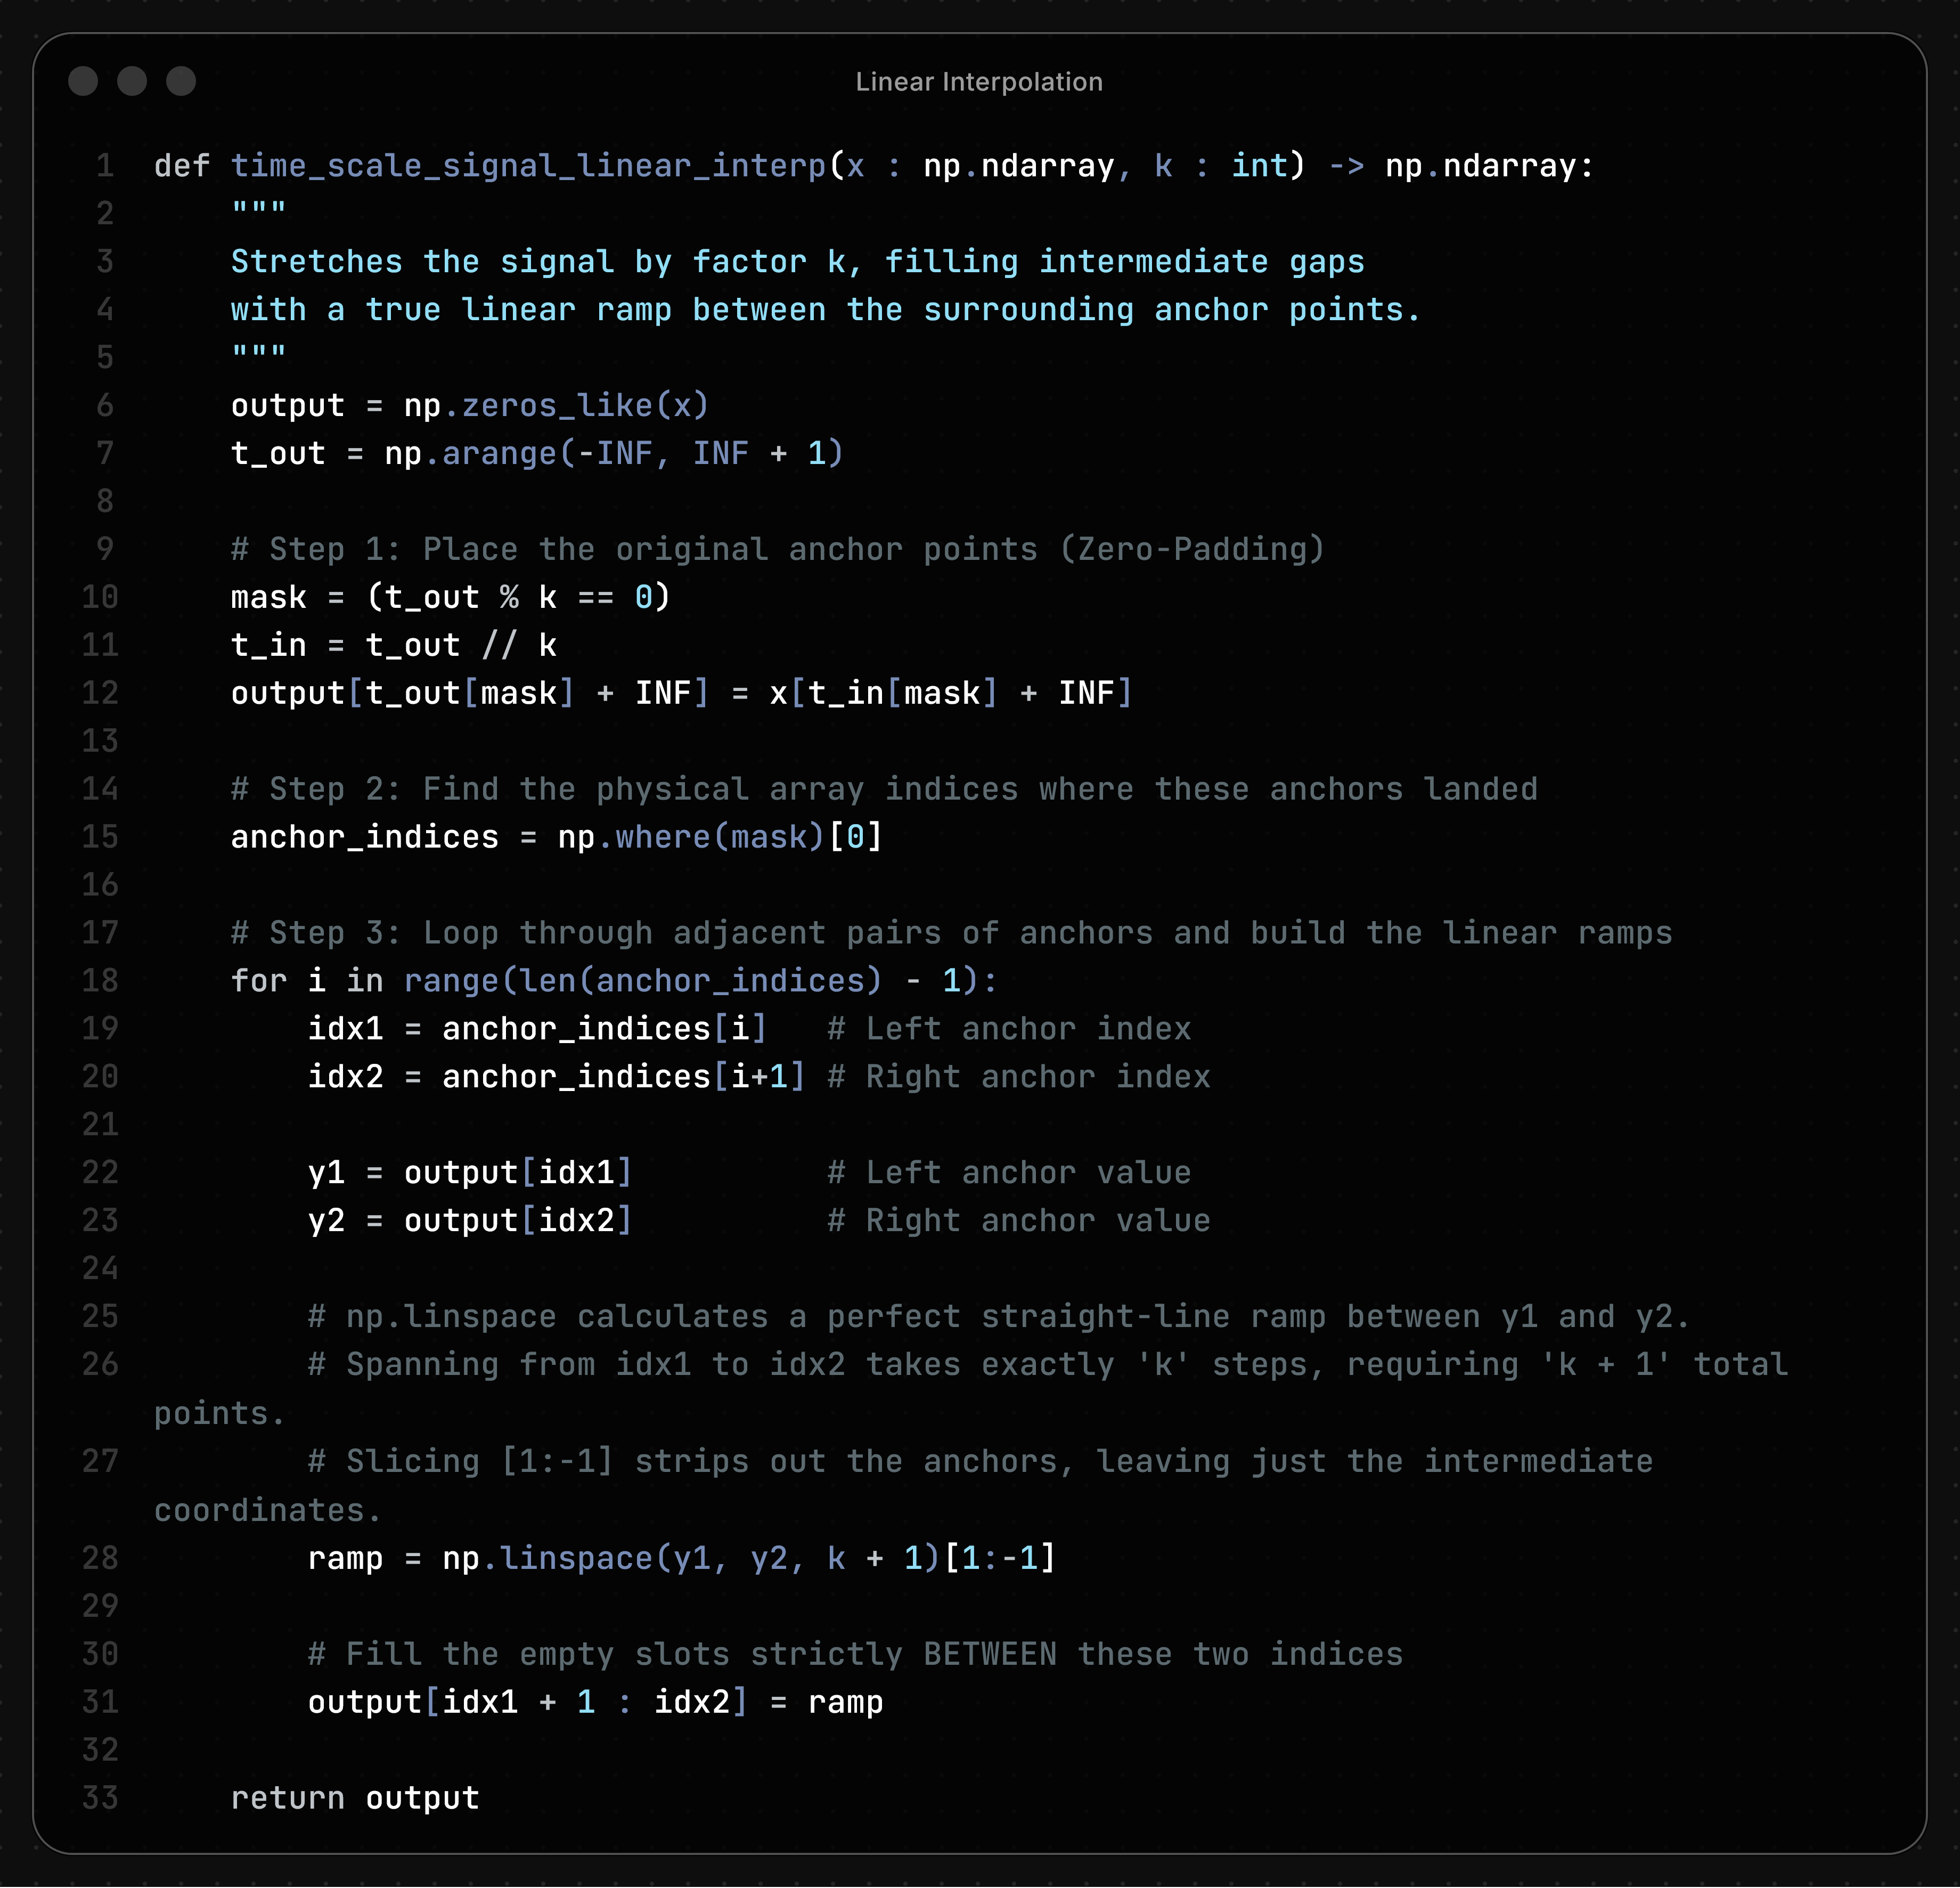
\includegraphics[width=\textwidth]{li.png}
    \subcaption{figure left}
    \end{minipage}\hfill
    \begin{minipage}{0.45\textwidth}
    \centering
    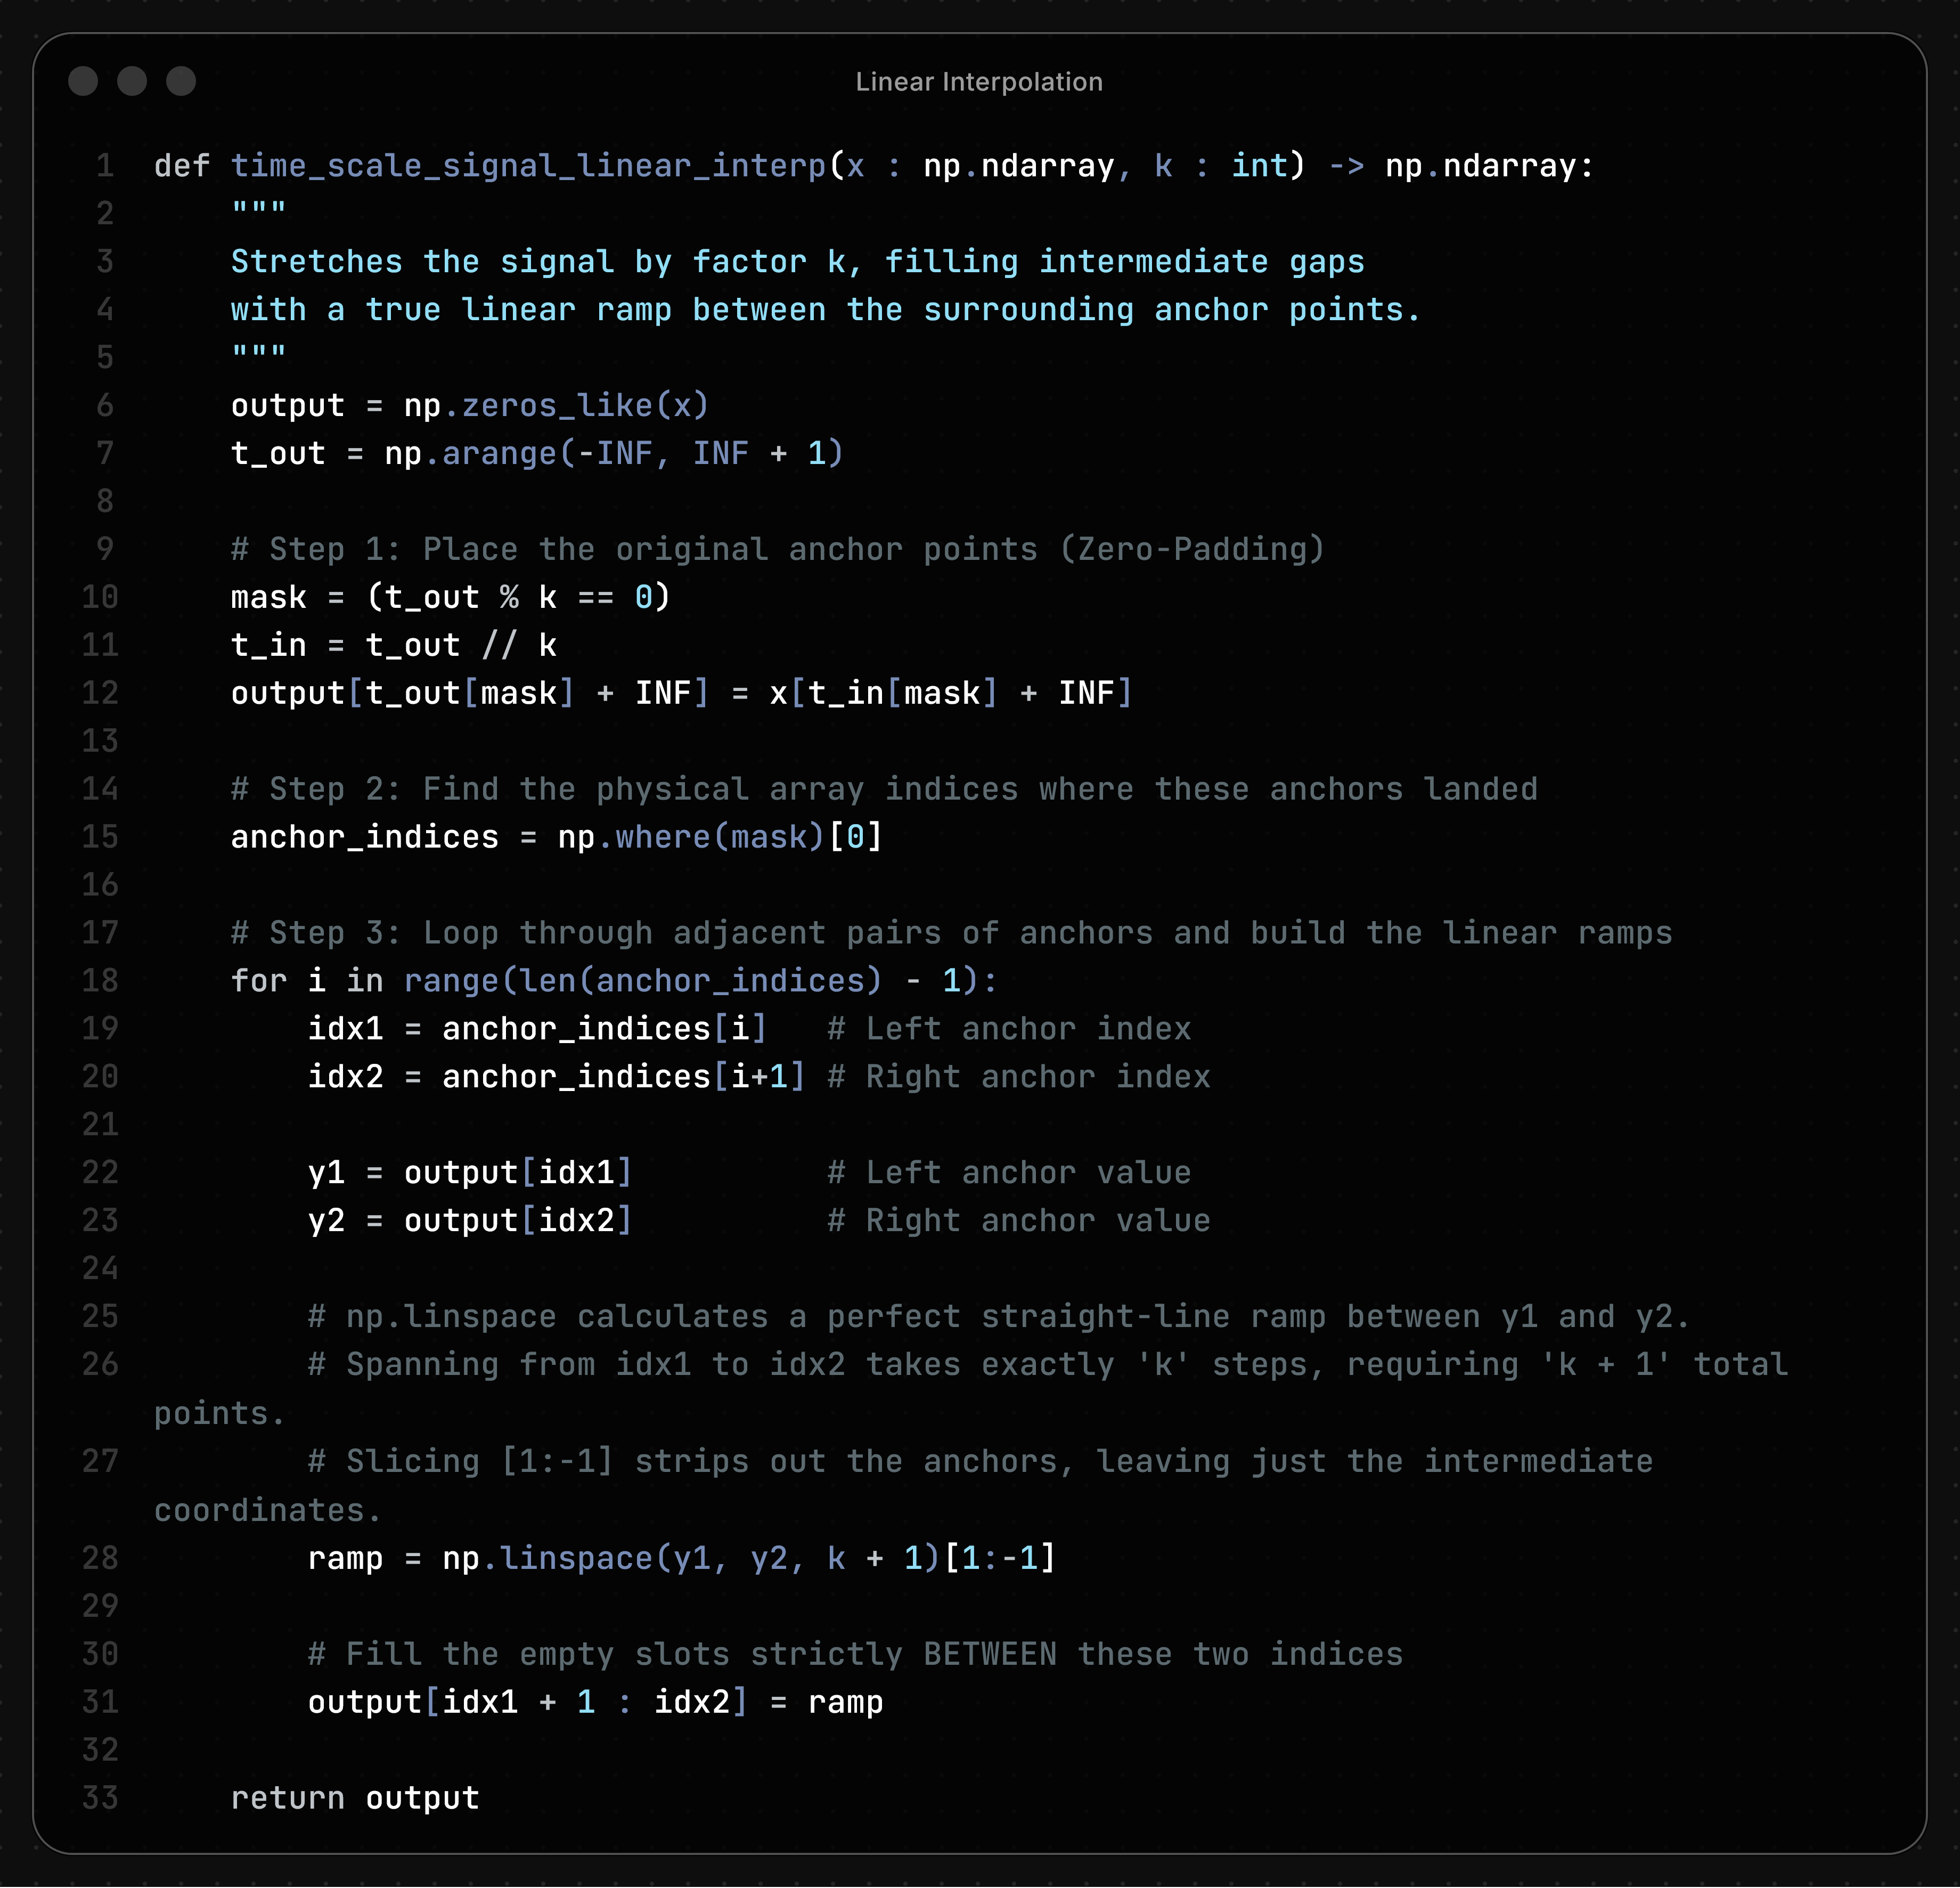
\includegraphics[width=\textwidth]{li.png}
    \subcaption{figure right}
    \end{minipage}
    \caption{whole figure}
\end{figure}

\section*{Ex 05}

\begin{wrapfigure}{r}{0.4\textwidth}
    \centering
    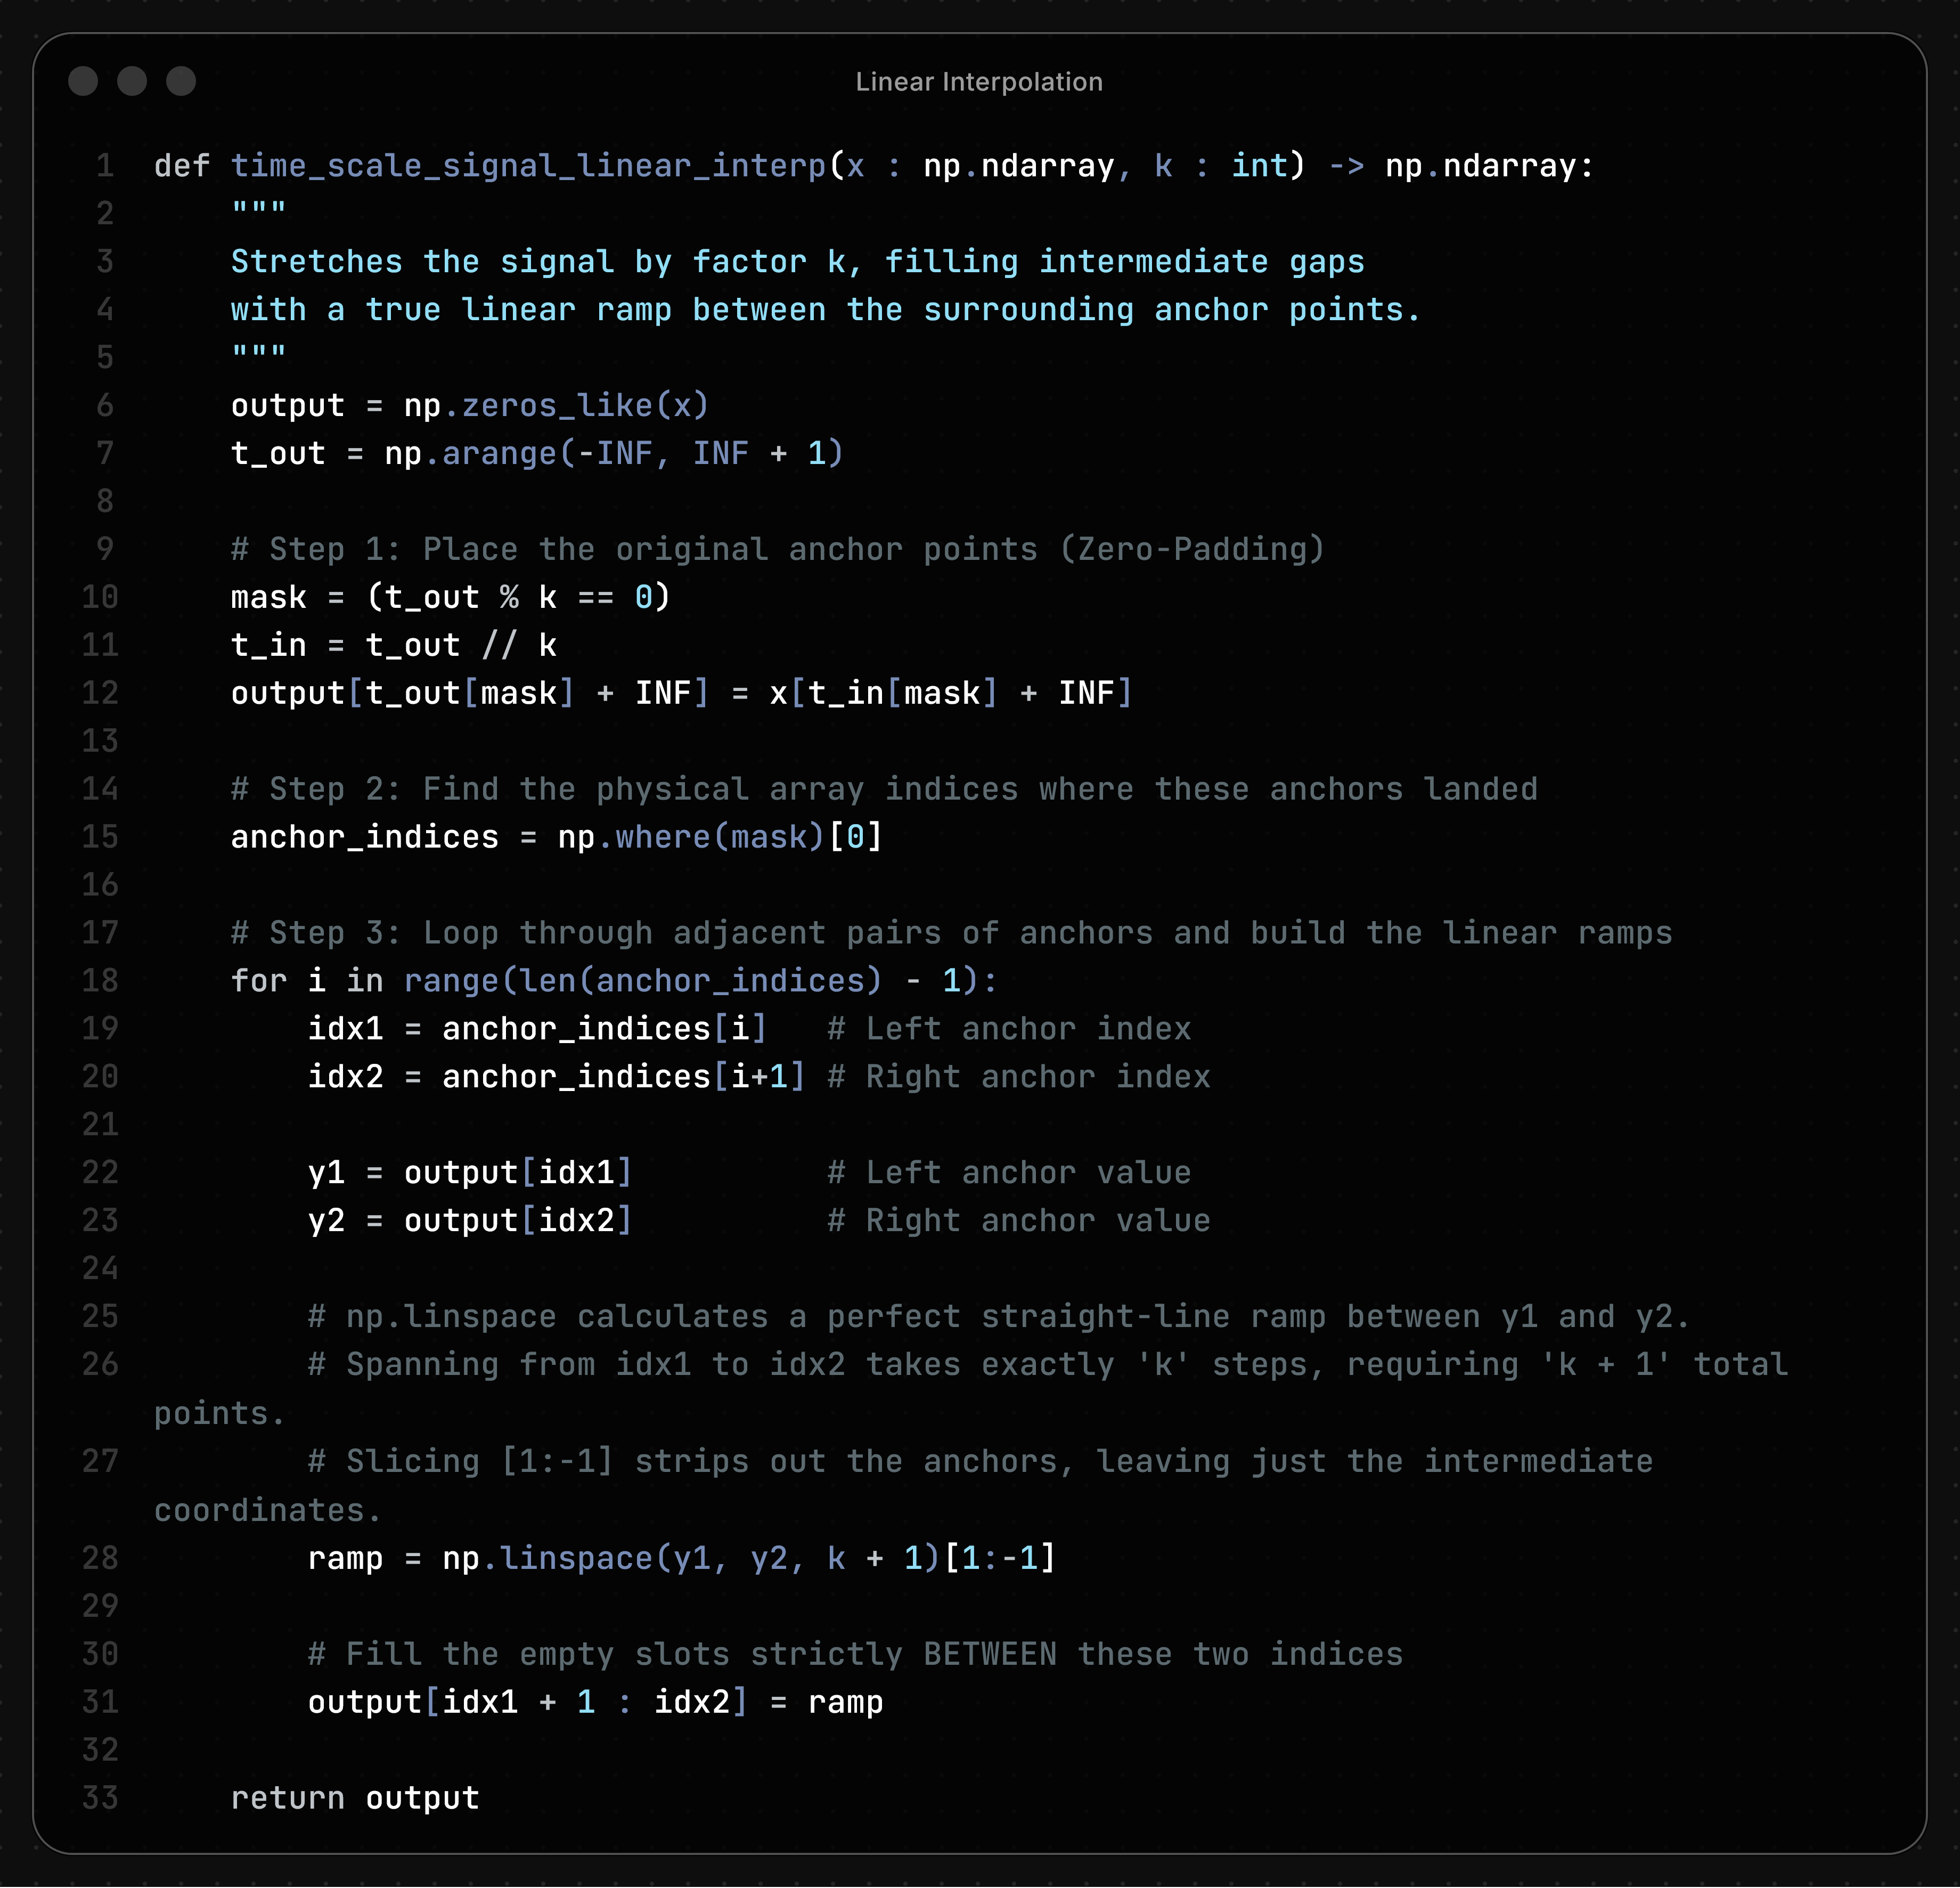
\includegraphics[width=\linewidth]{li.png}
    \caption{A wrapped figure n the right}
    \label{fig:wrapp}
\end{wrapfigure}

\lipsum[1-2]

\begin{wrapfigure}{r}{0.38\textwidth} % r = right, l = left
\centering
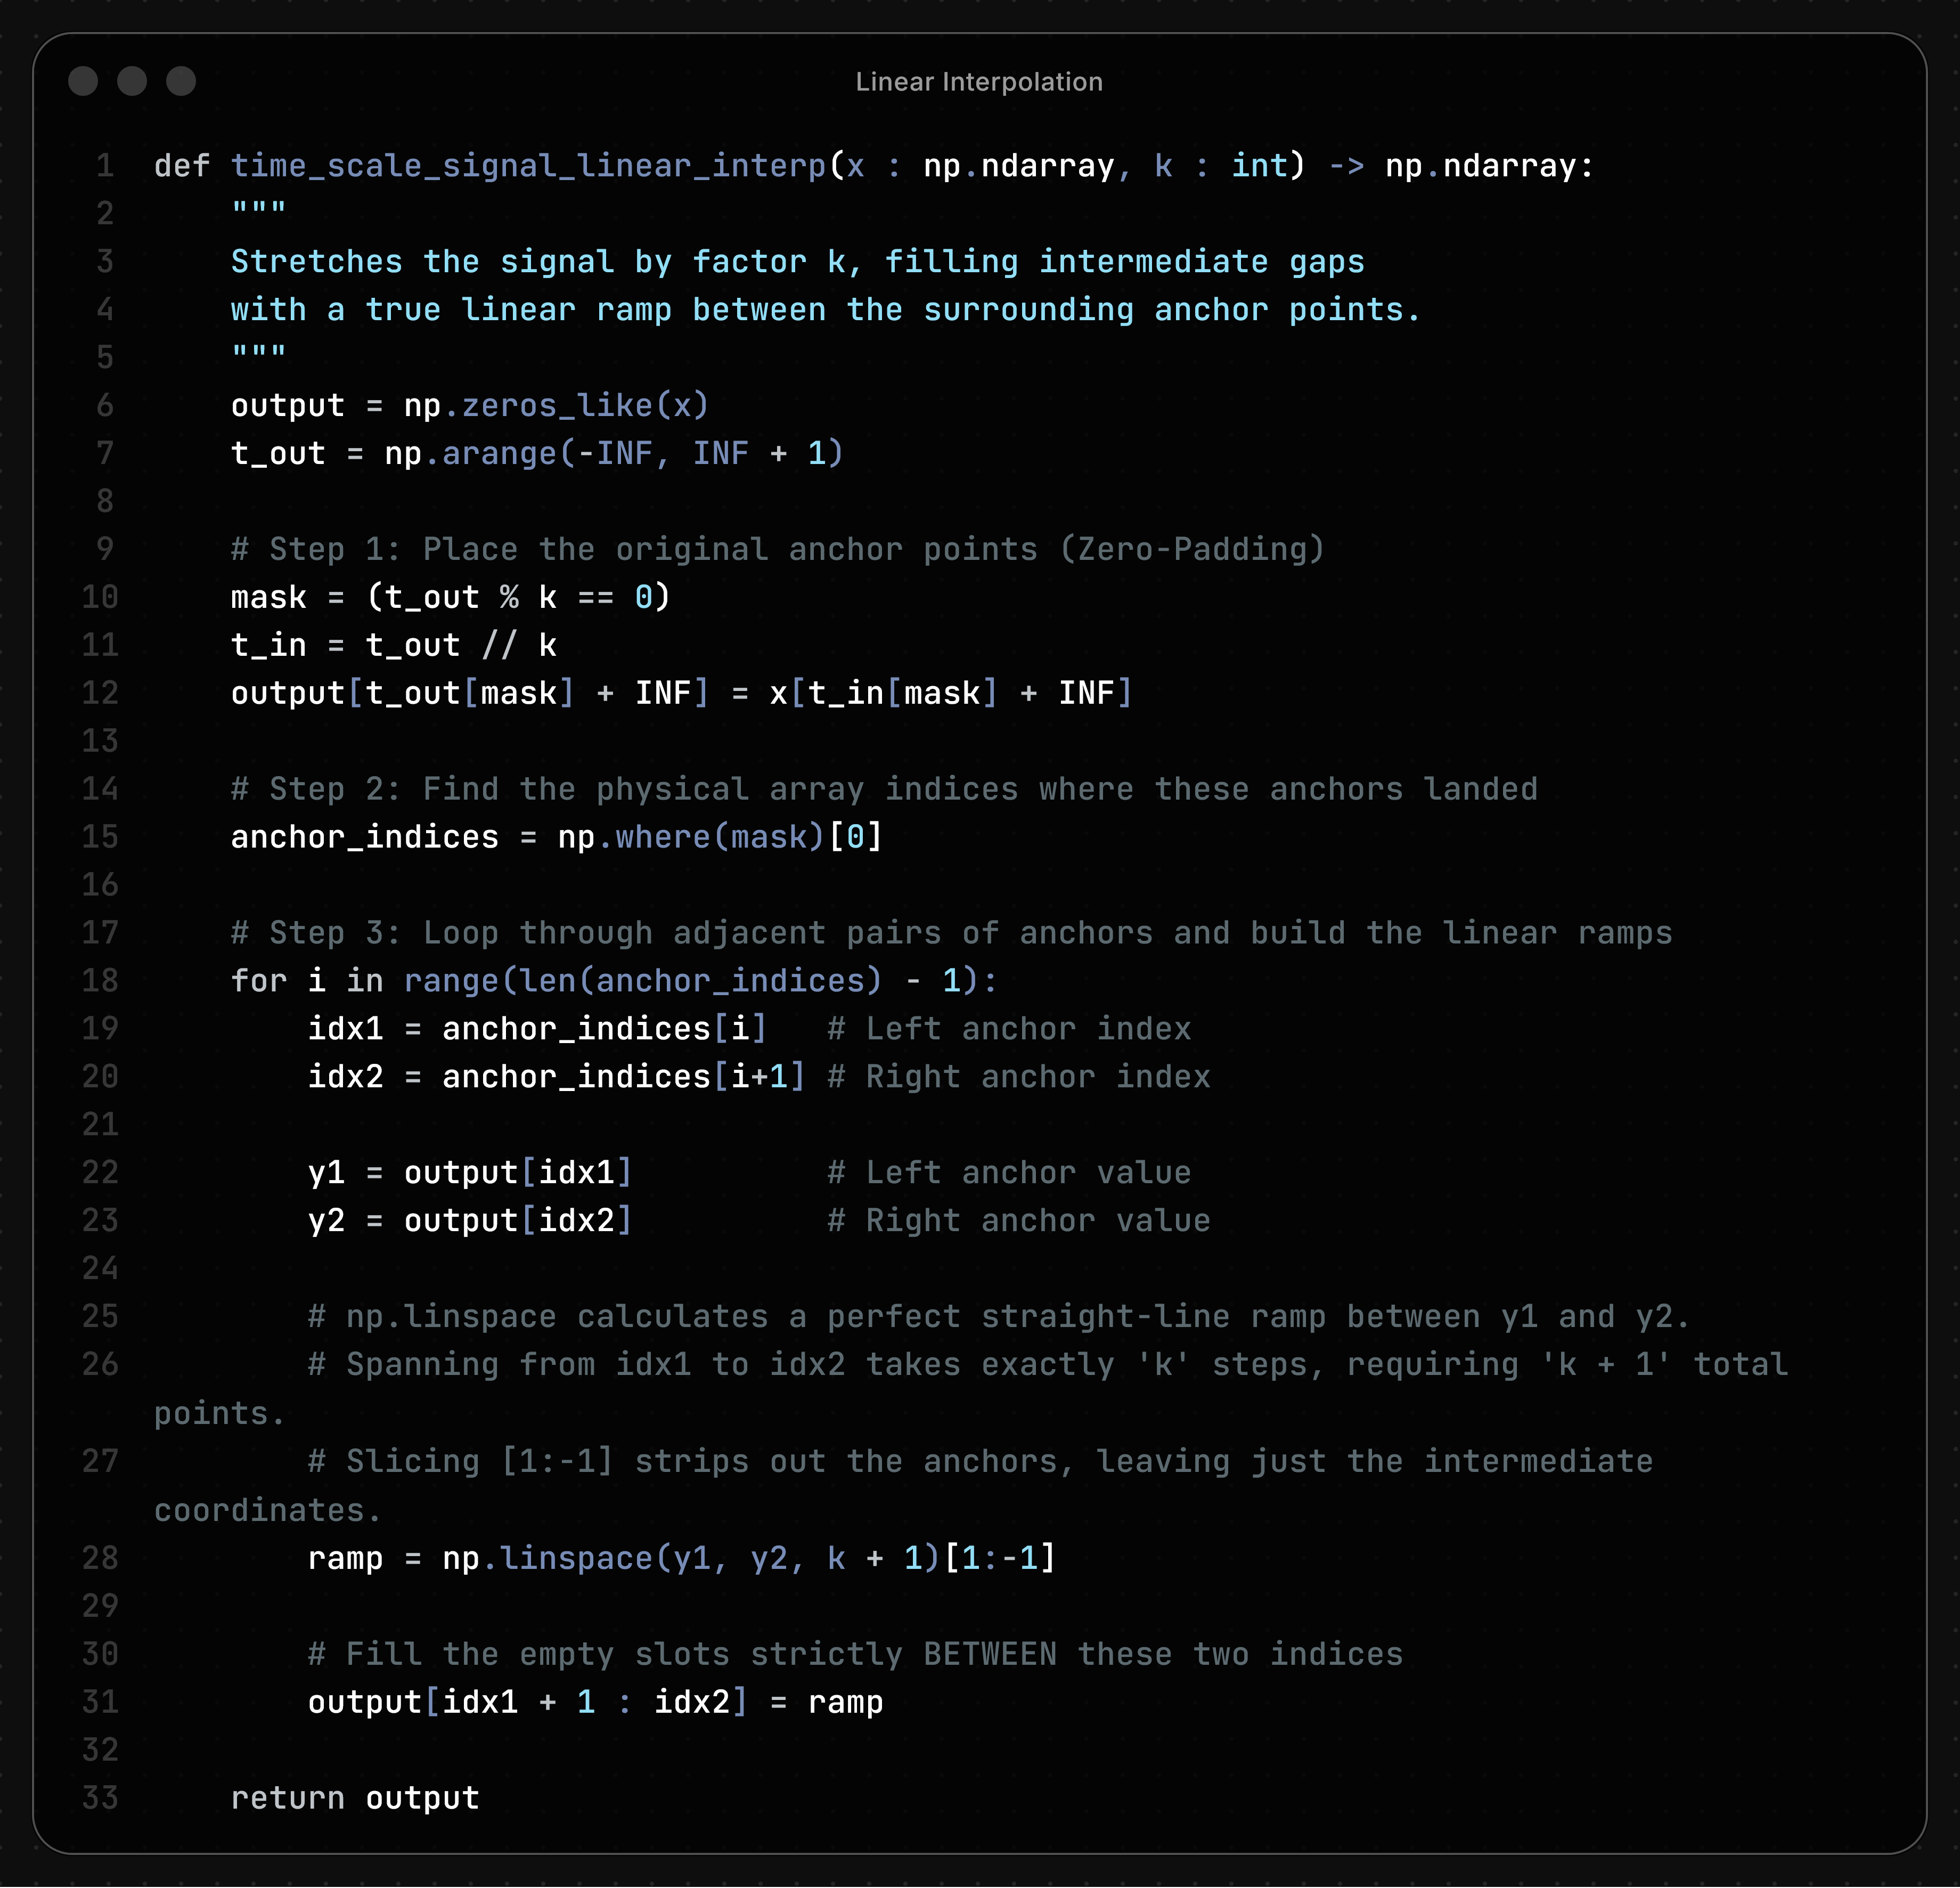
\includegraphics[width=\linewidth]{li.png}
\caption{A wrapped figure on the right.}
\label{fig:wrap}
\end{wrapfigure}

Figure~\ref{fig:wrap} sits on the right while this paragraph flows
around it. Lorem ipsum ... (enough text to fill the figure’s height)\newline
\lipsum[1-2]

\section*{Ex 08}

% \begin{figure}
    
%     \begin{subfigure}[b][0.2\textwidth]
%         \centering
%         \fbox{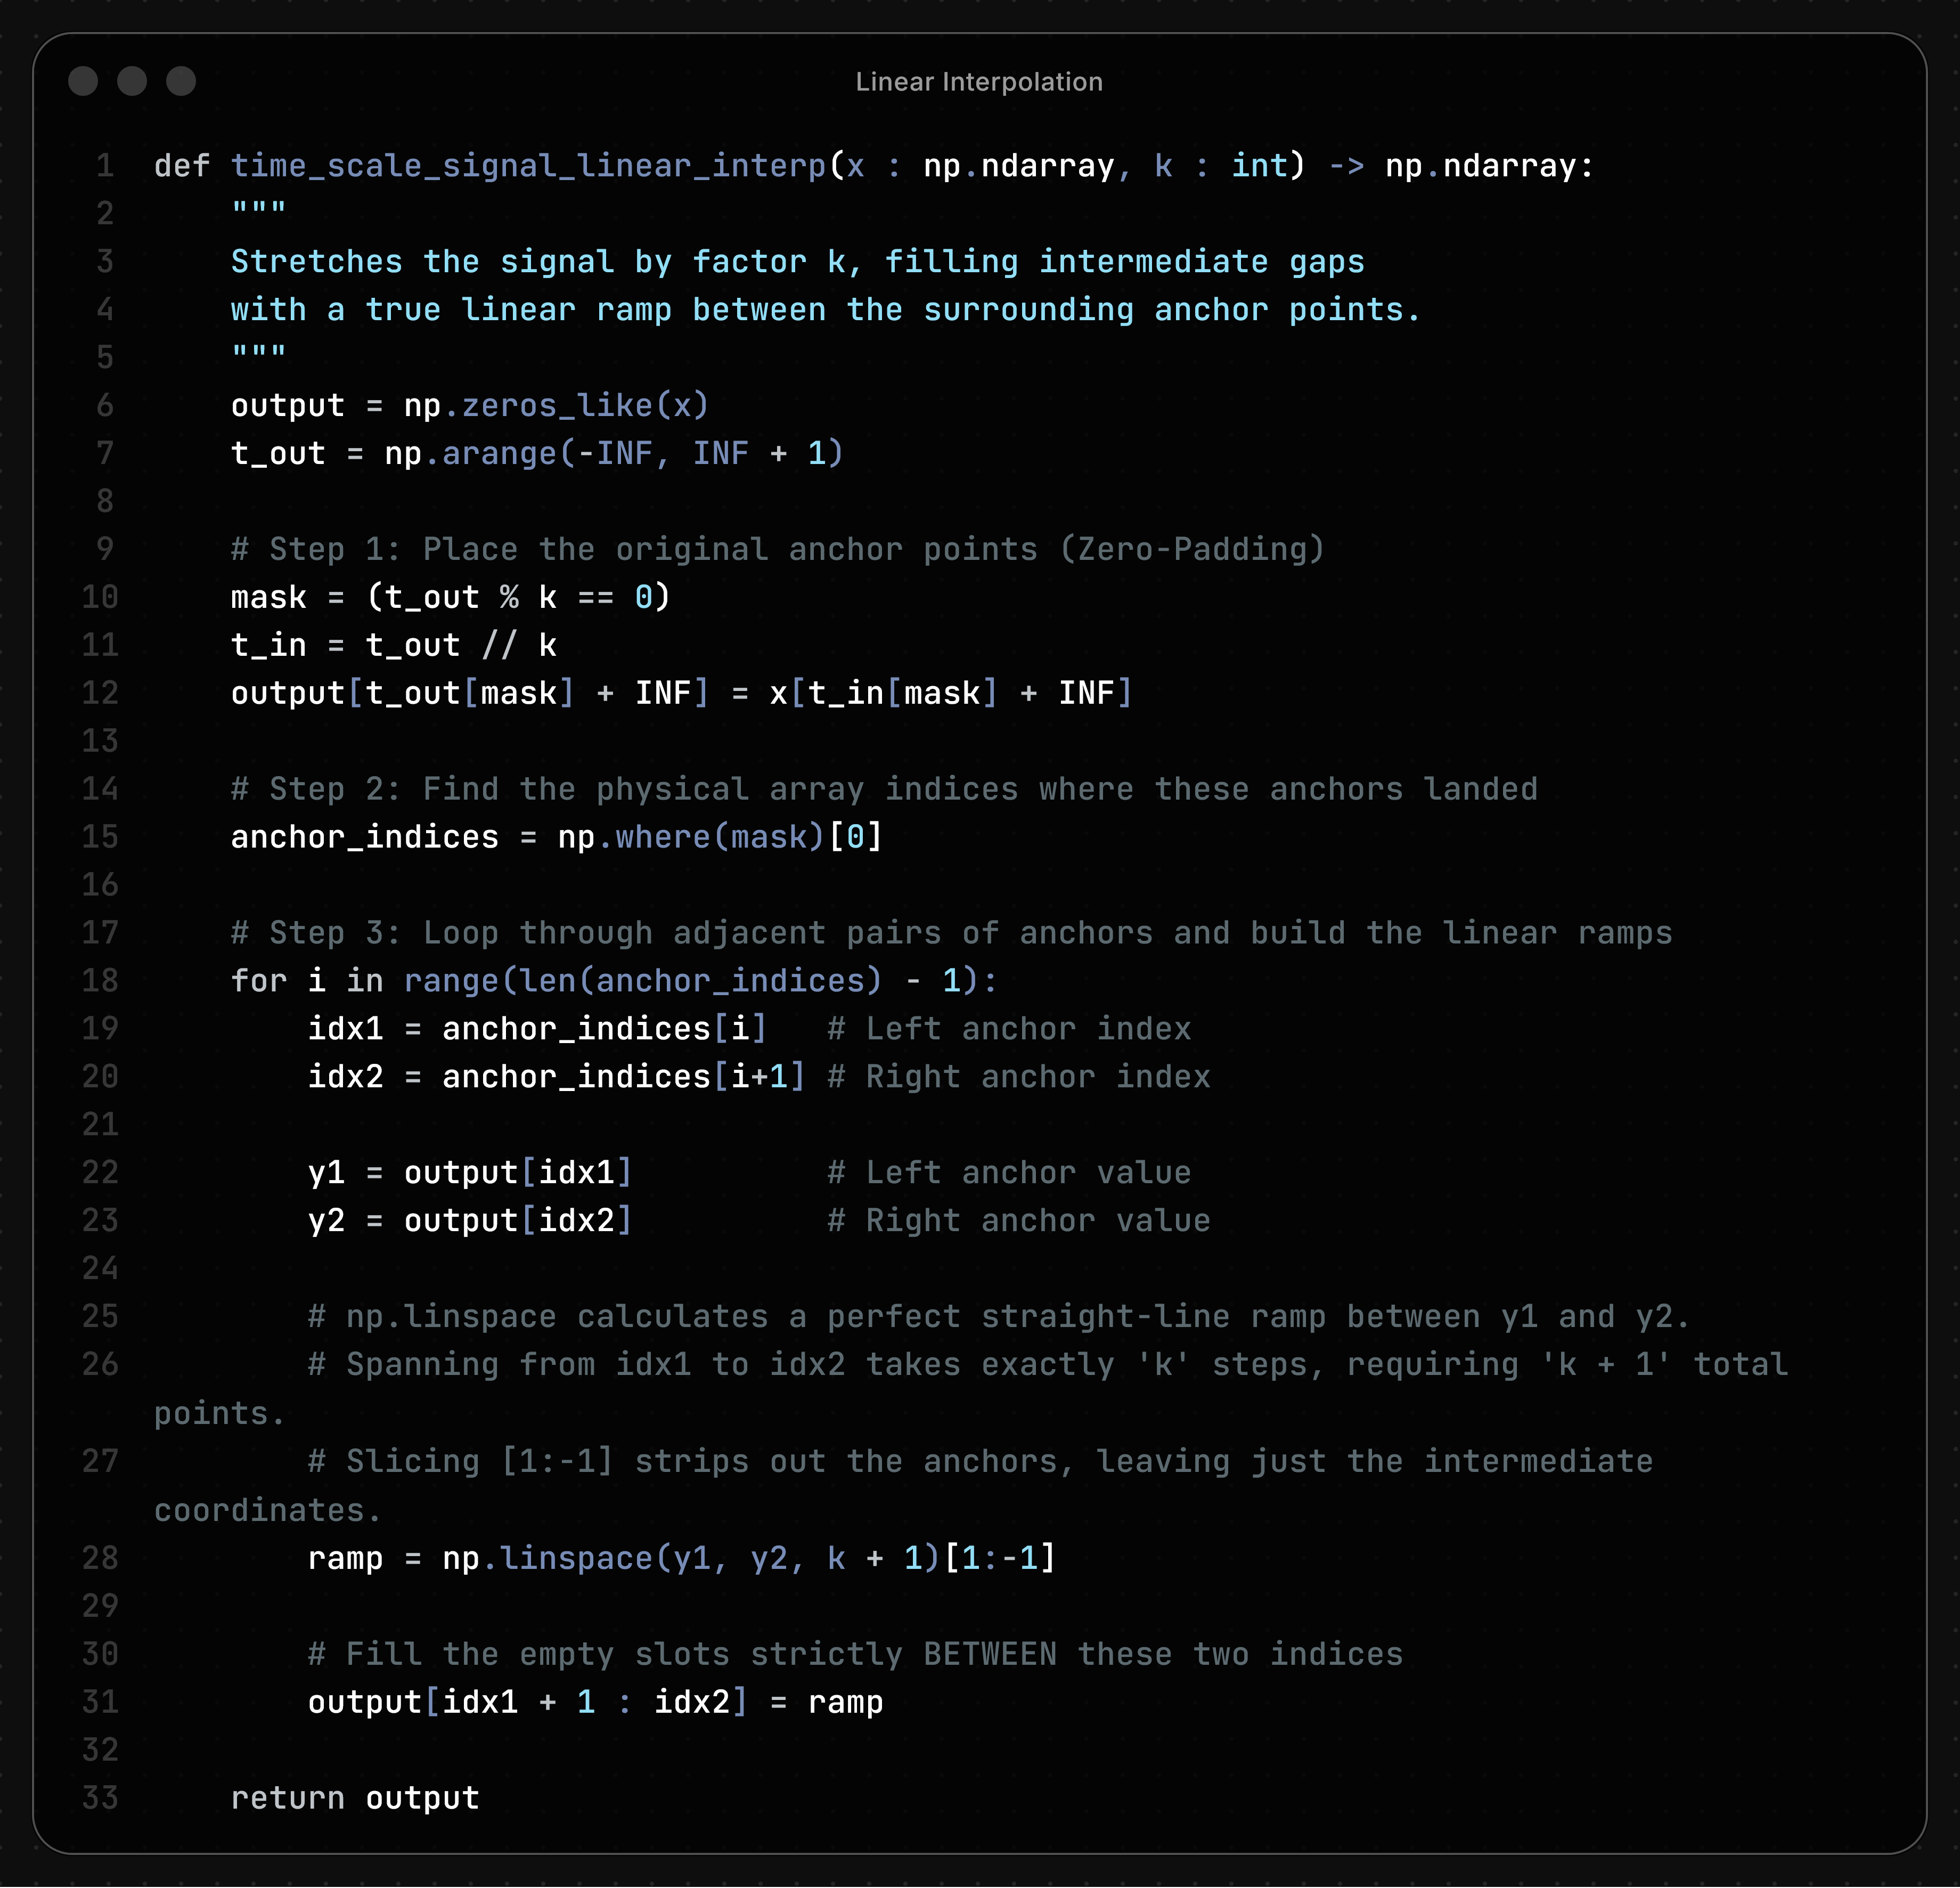
\includegraphics[width=\linewidth]{li.png}} % framed
%     \end{subfigure}\hfill
%     \begin{subfigure}[b][0.2\textwidth]
%         \centering
%         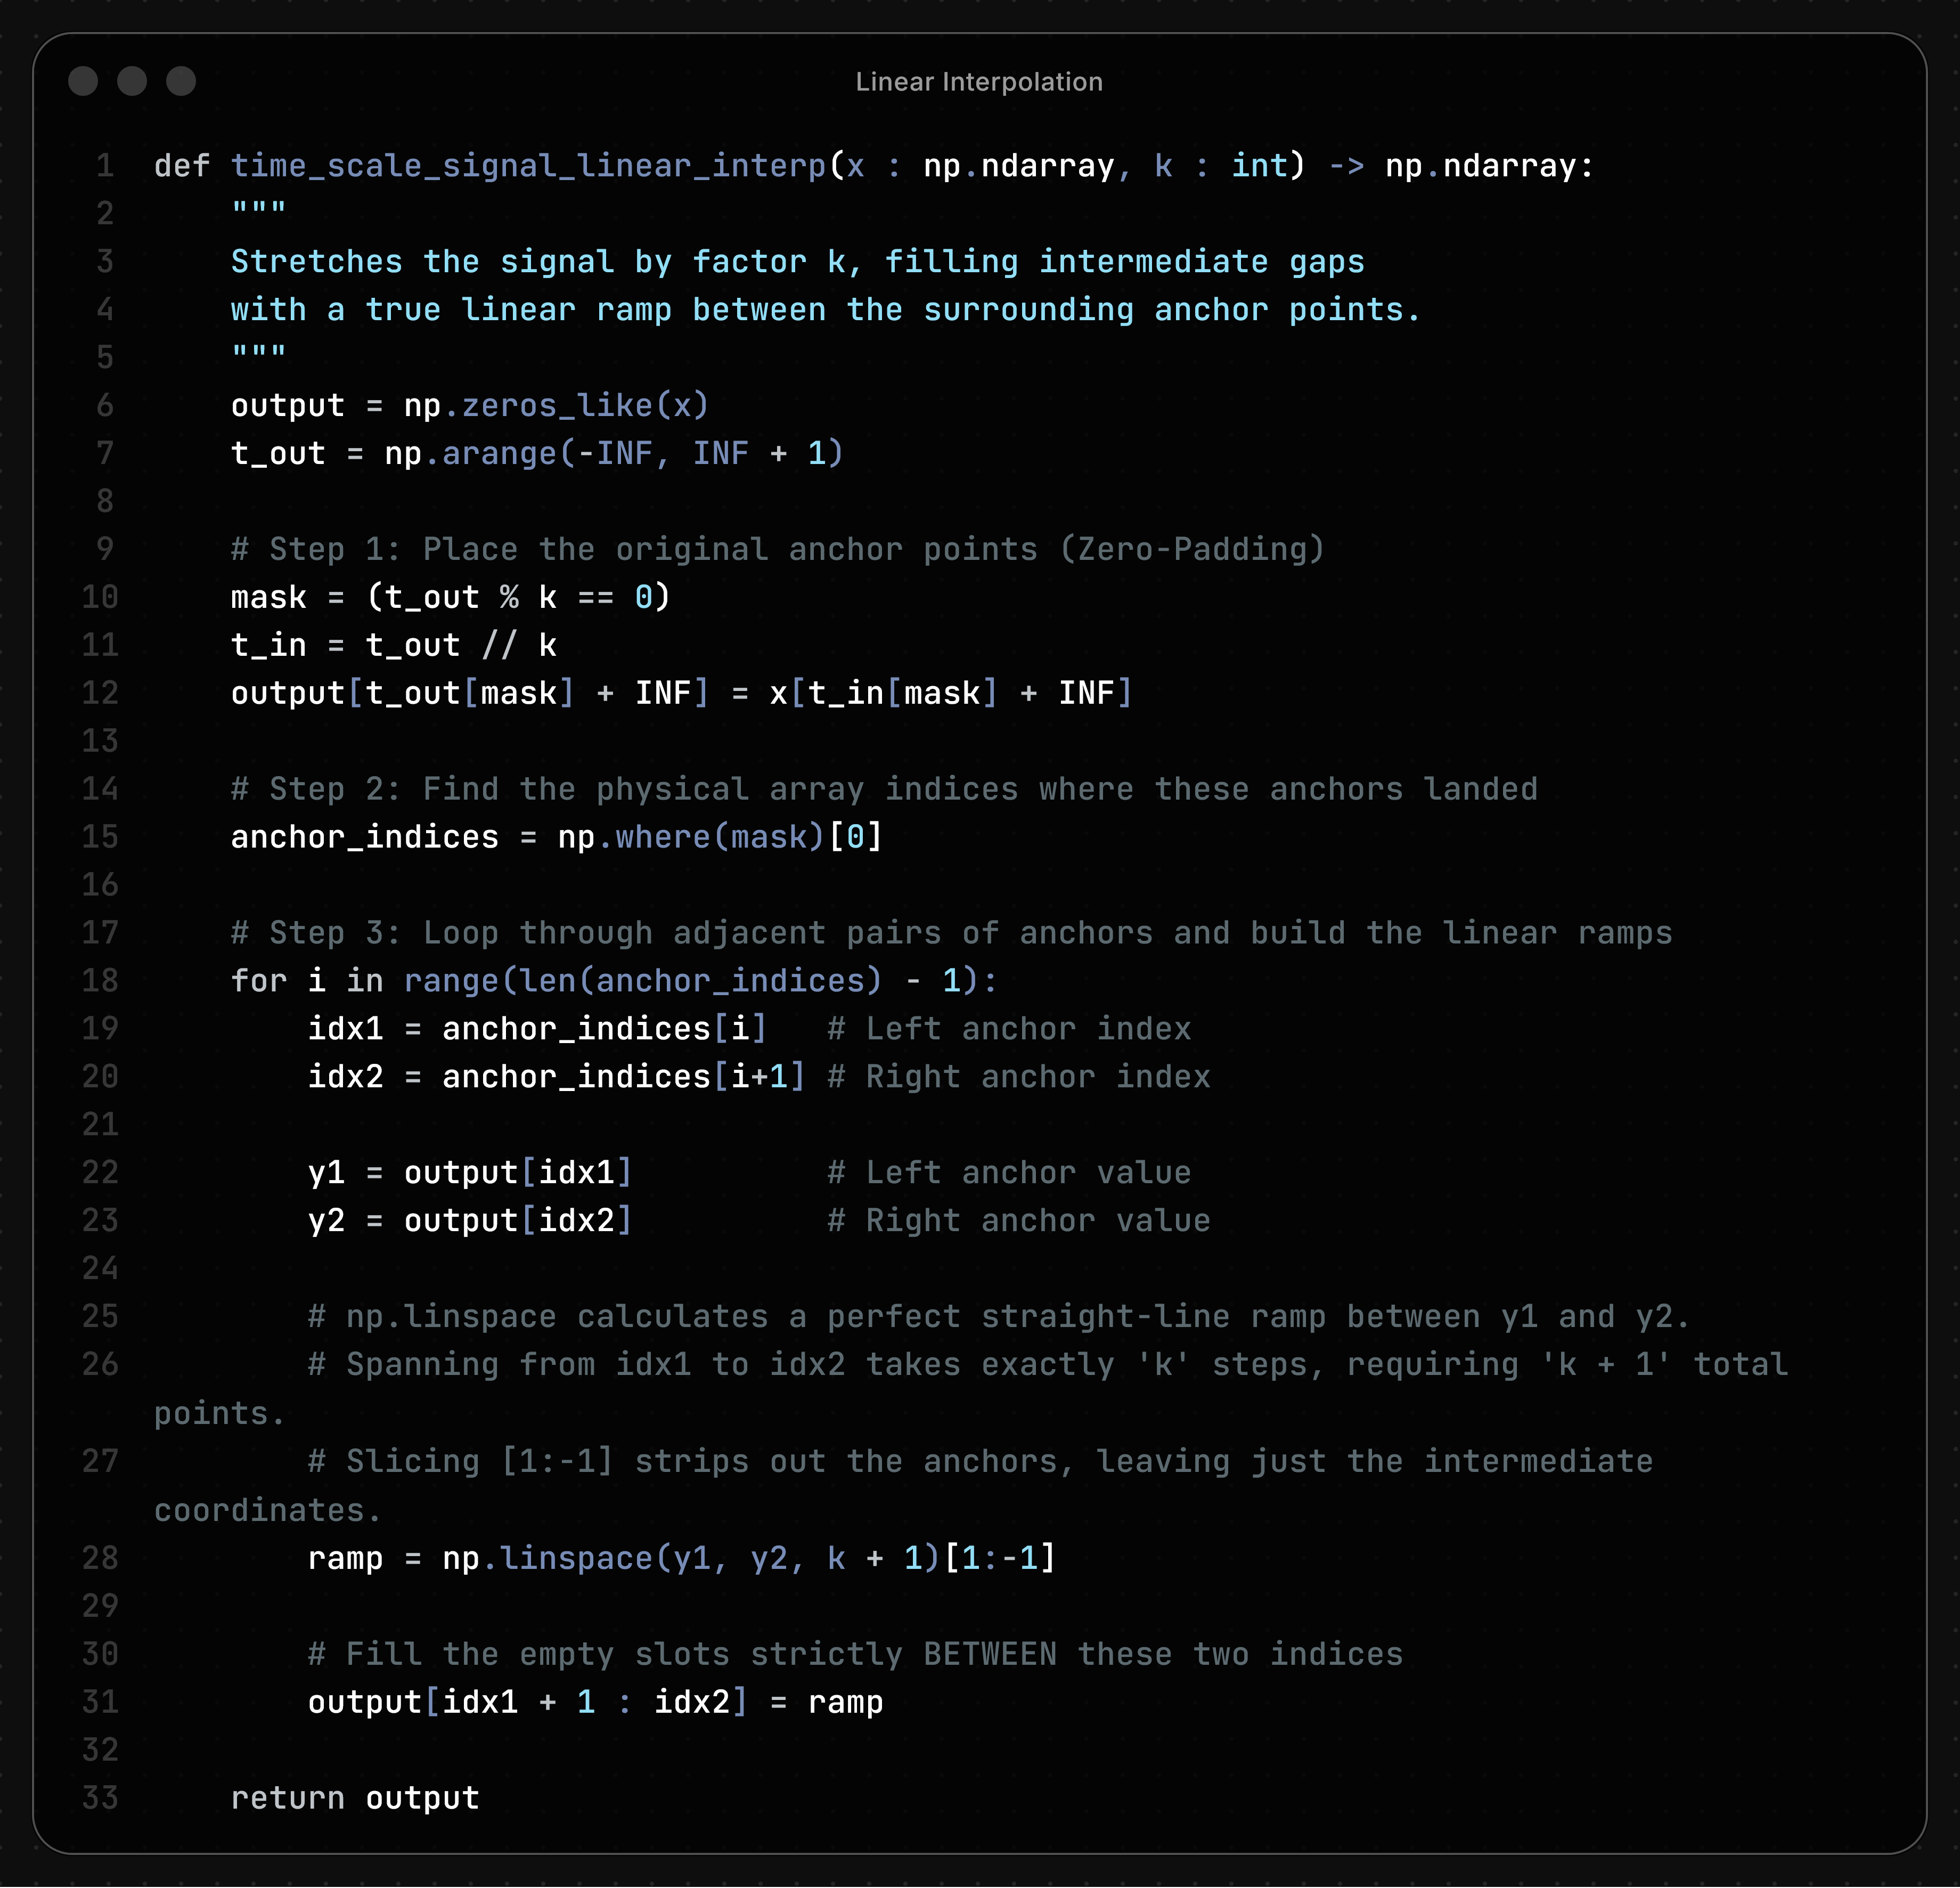
\includegraphics[height=2.2cm, keepaspectratio]{li.png} % fixed height
%     \end{subfigure}\hfill
%     \begin{subfigure}[b][0.2\textwidth]
%         \centering
%         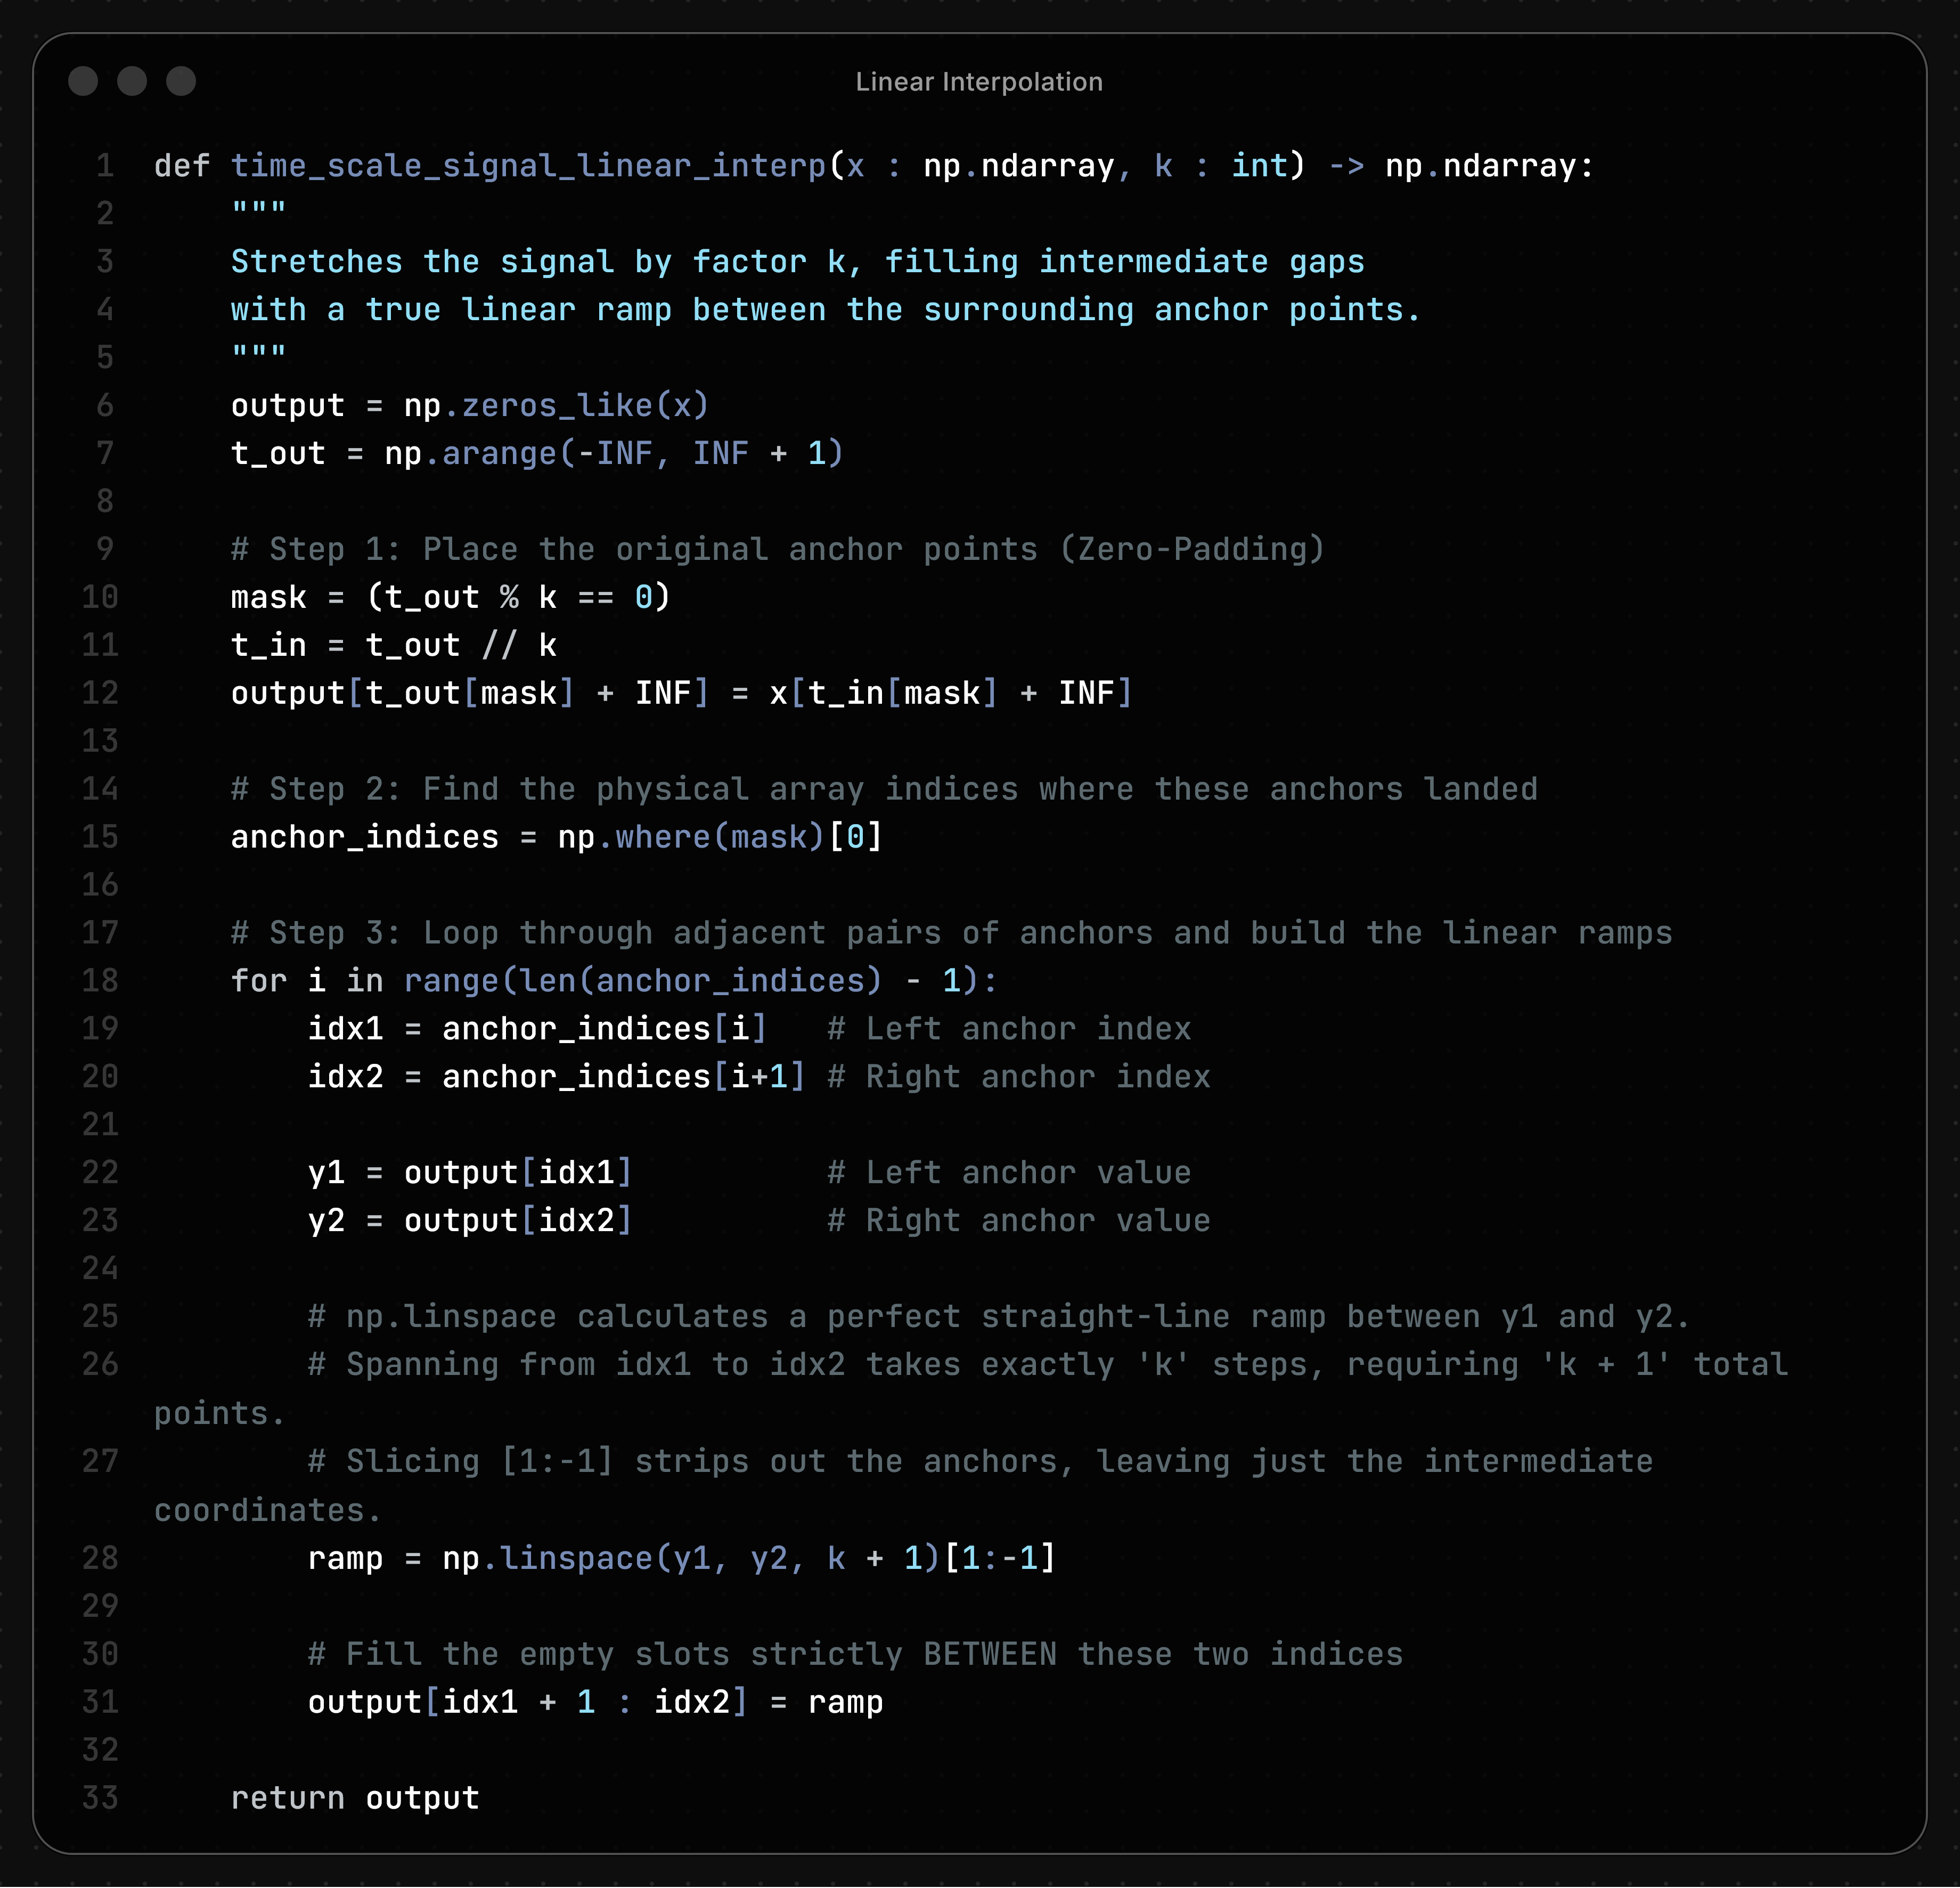
\includegraphics[width=\linewidth, trim=2cm 1cm 2cm 1cm, clip]{li.png}
%     \end{subfigure}\hfill
%     \begin{subfigure}[b][0.2\textwidth]
%         \resizebox{\linewidth}{2.2cm}{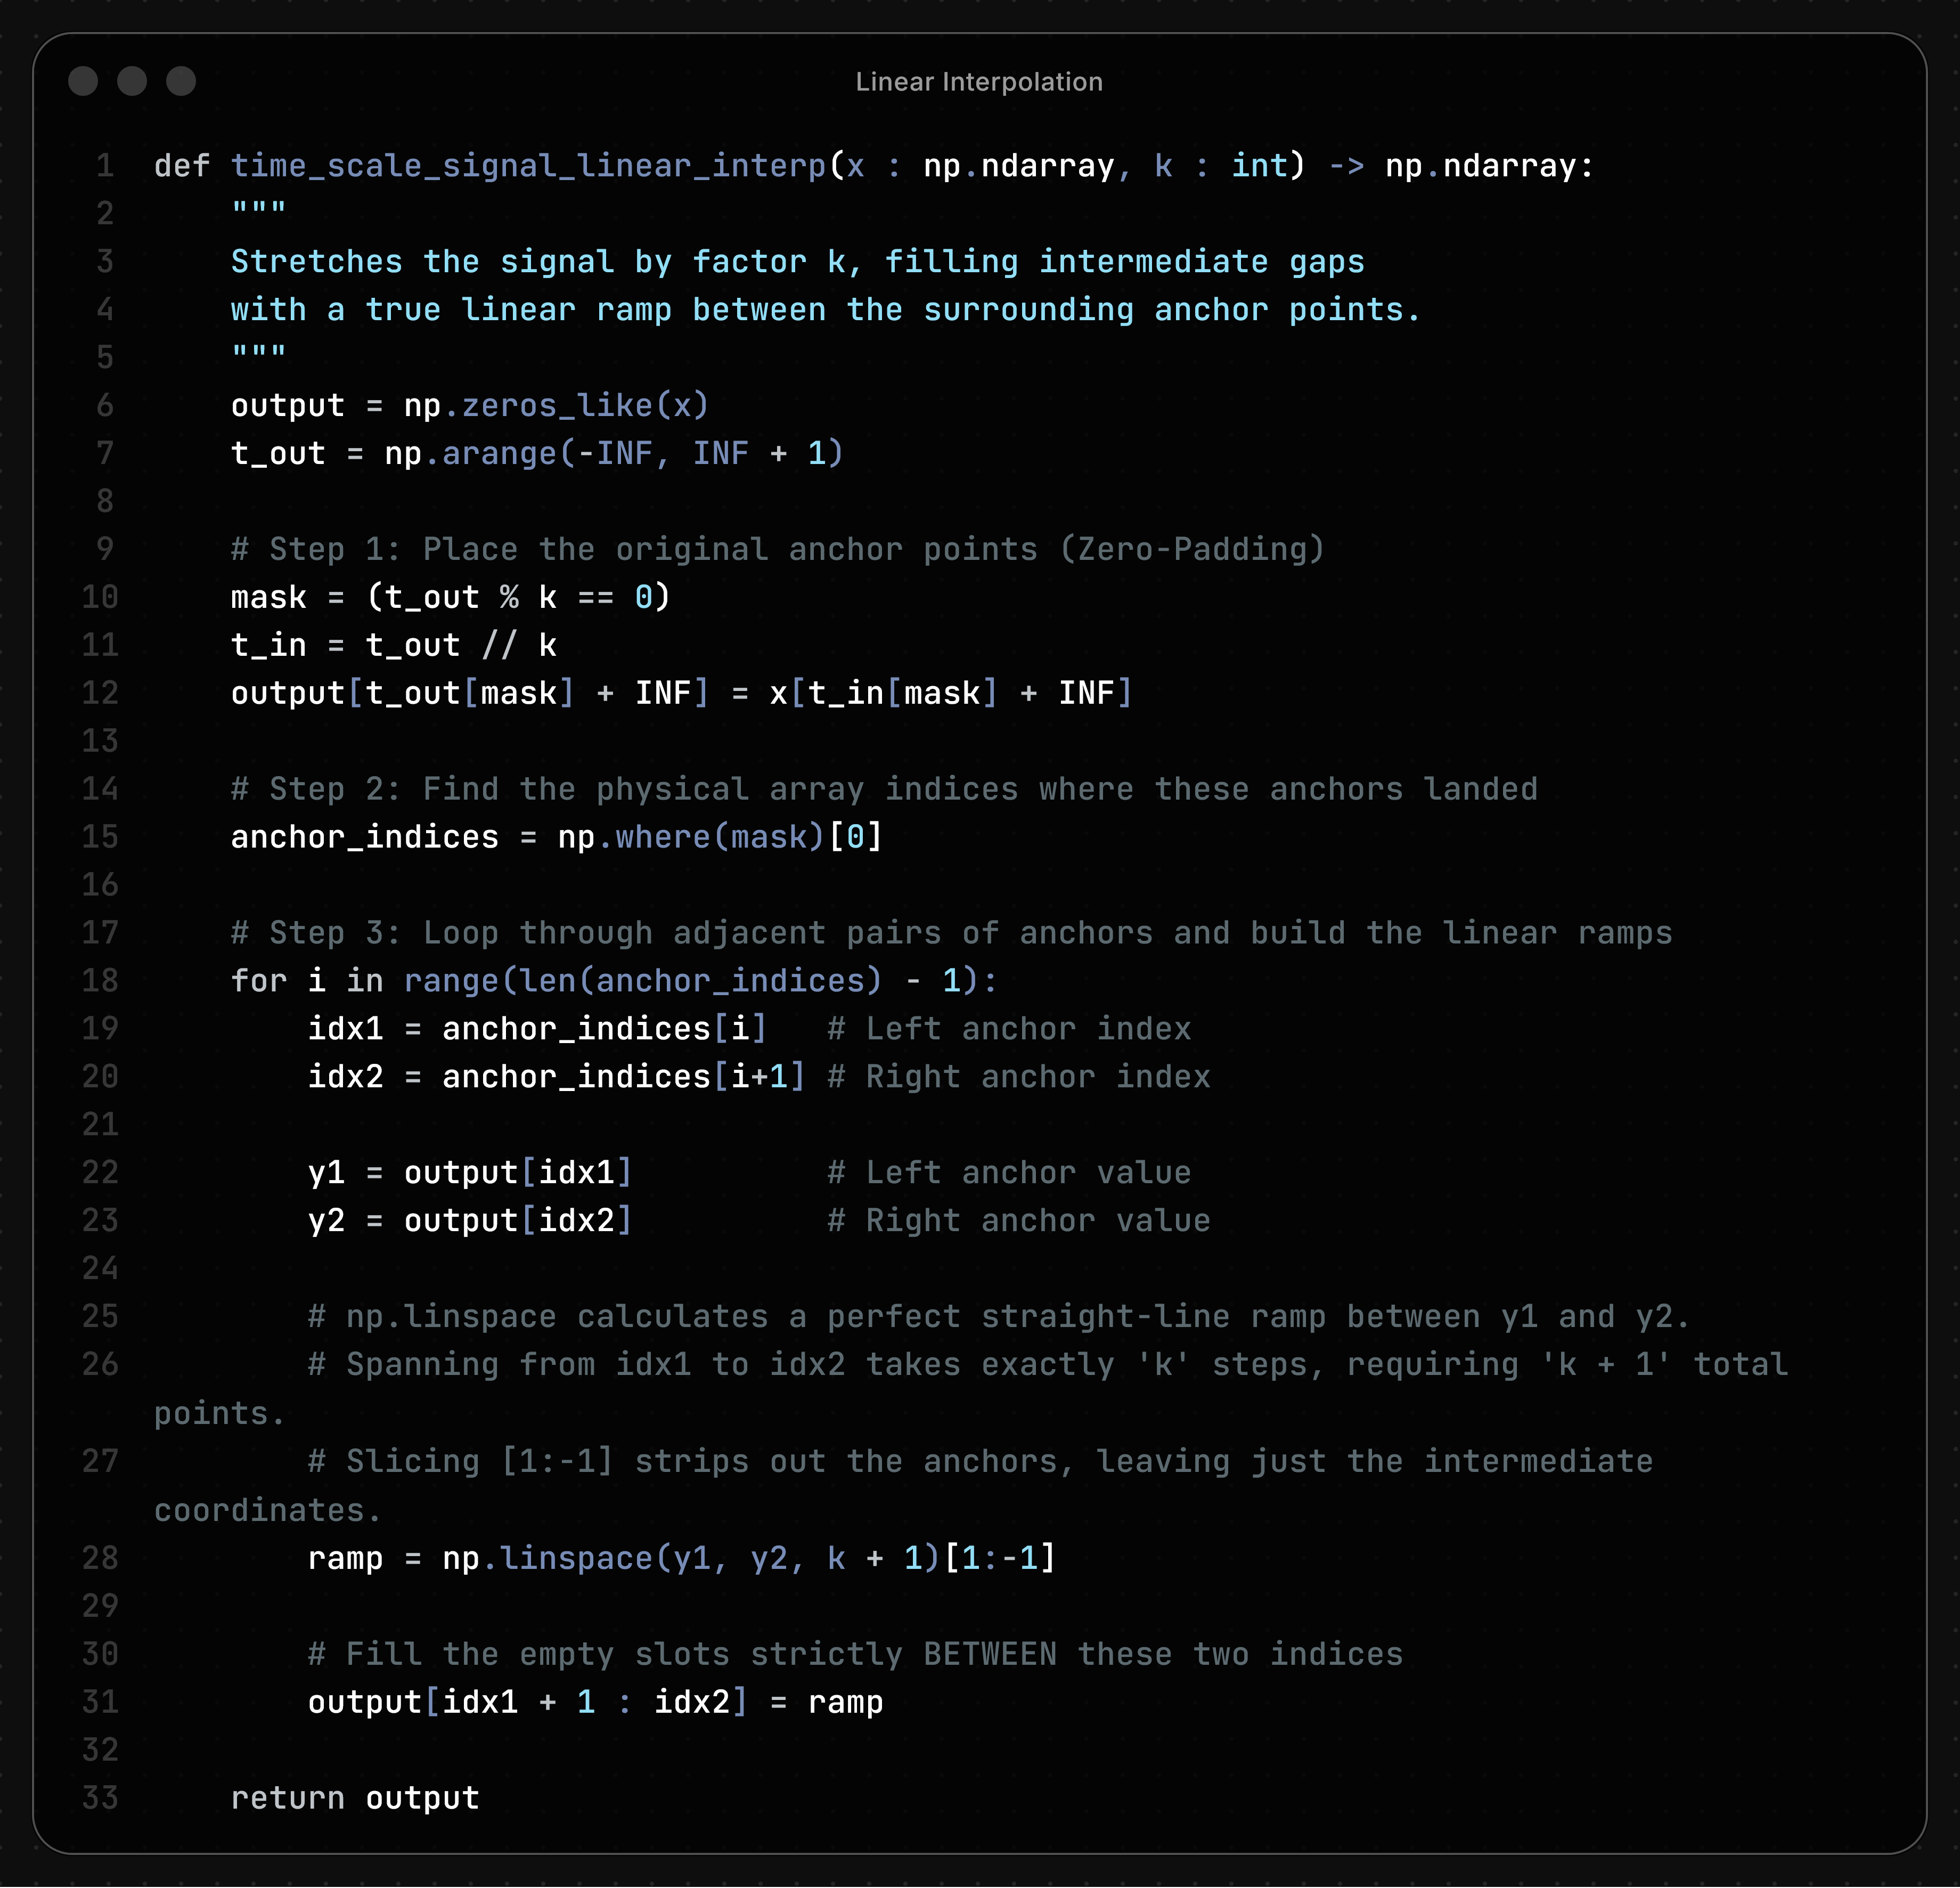
\includegraphics{li.png}} % stretched
%     \end{subfigure}


% \end{figure}


\begin{figure}[htbp]
    \centering
    \begin{subfigure}[b]{0.2\textwidth}
        \centering
        \fbox{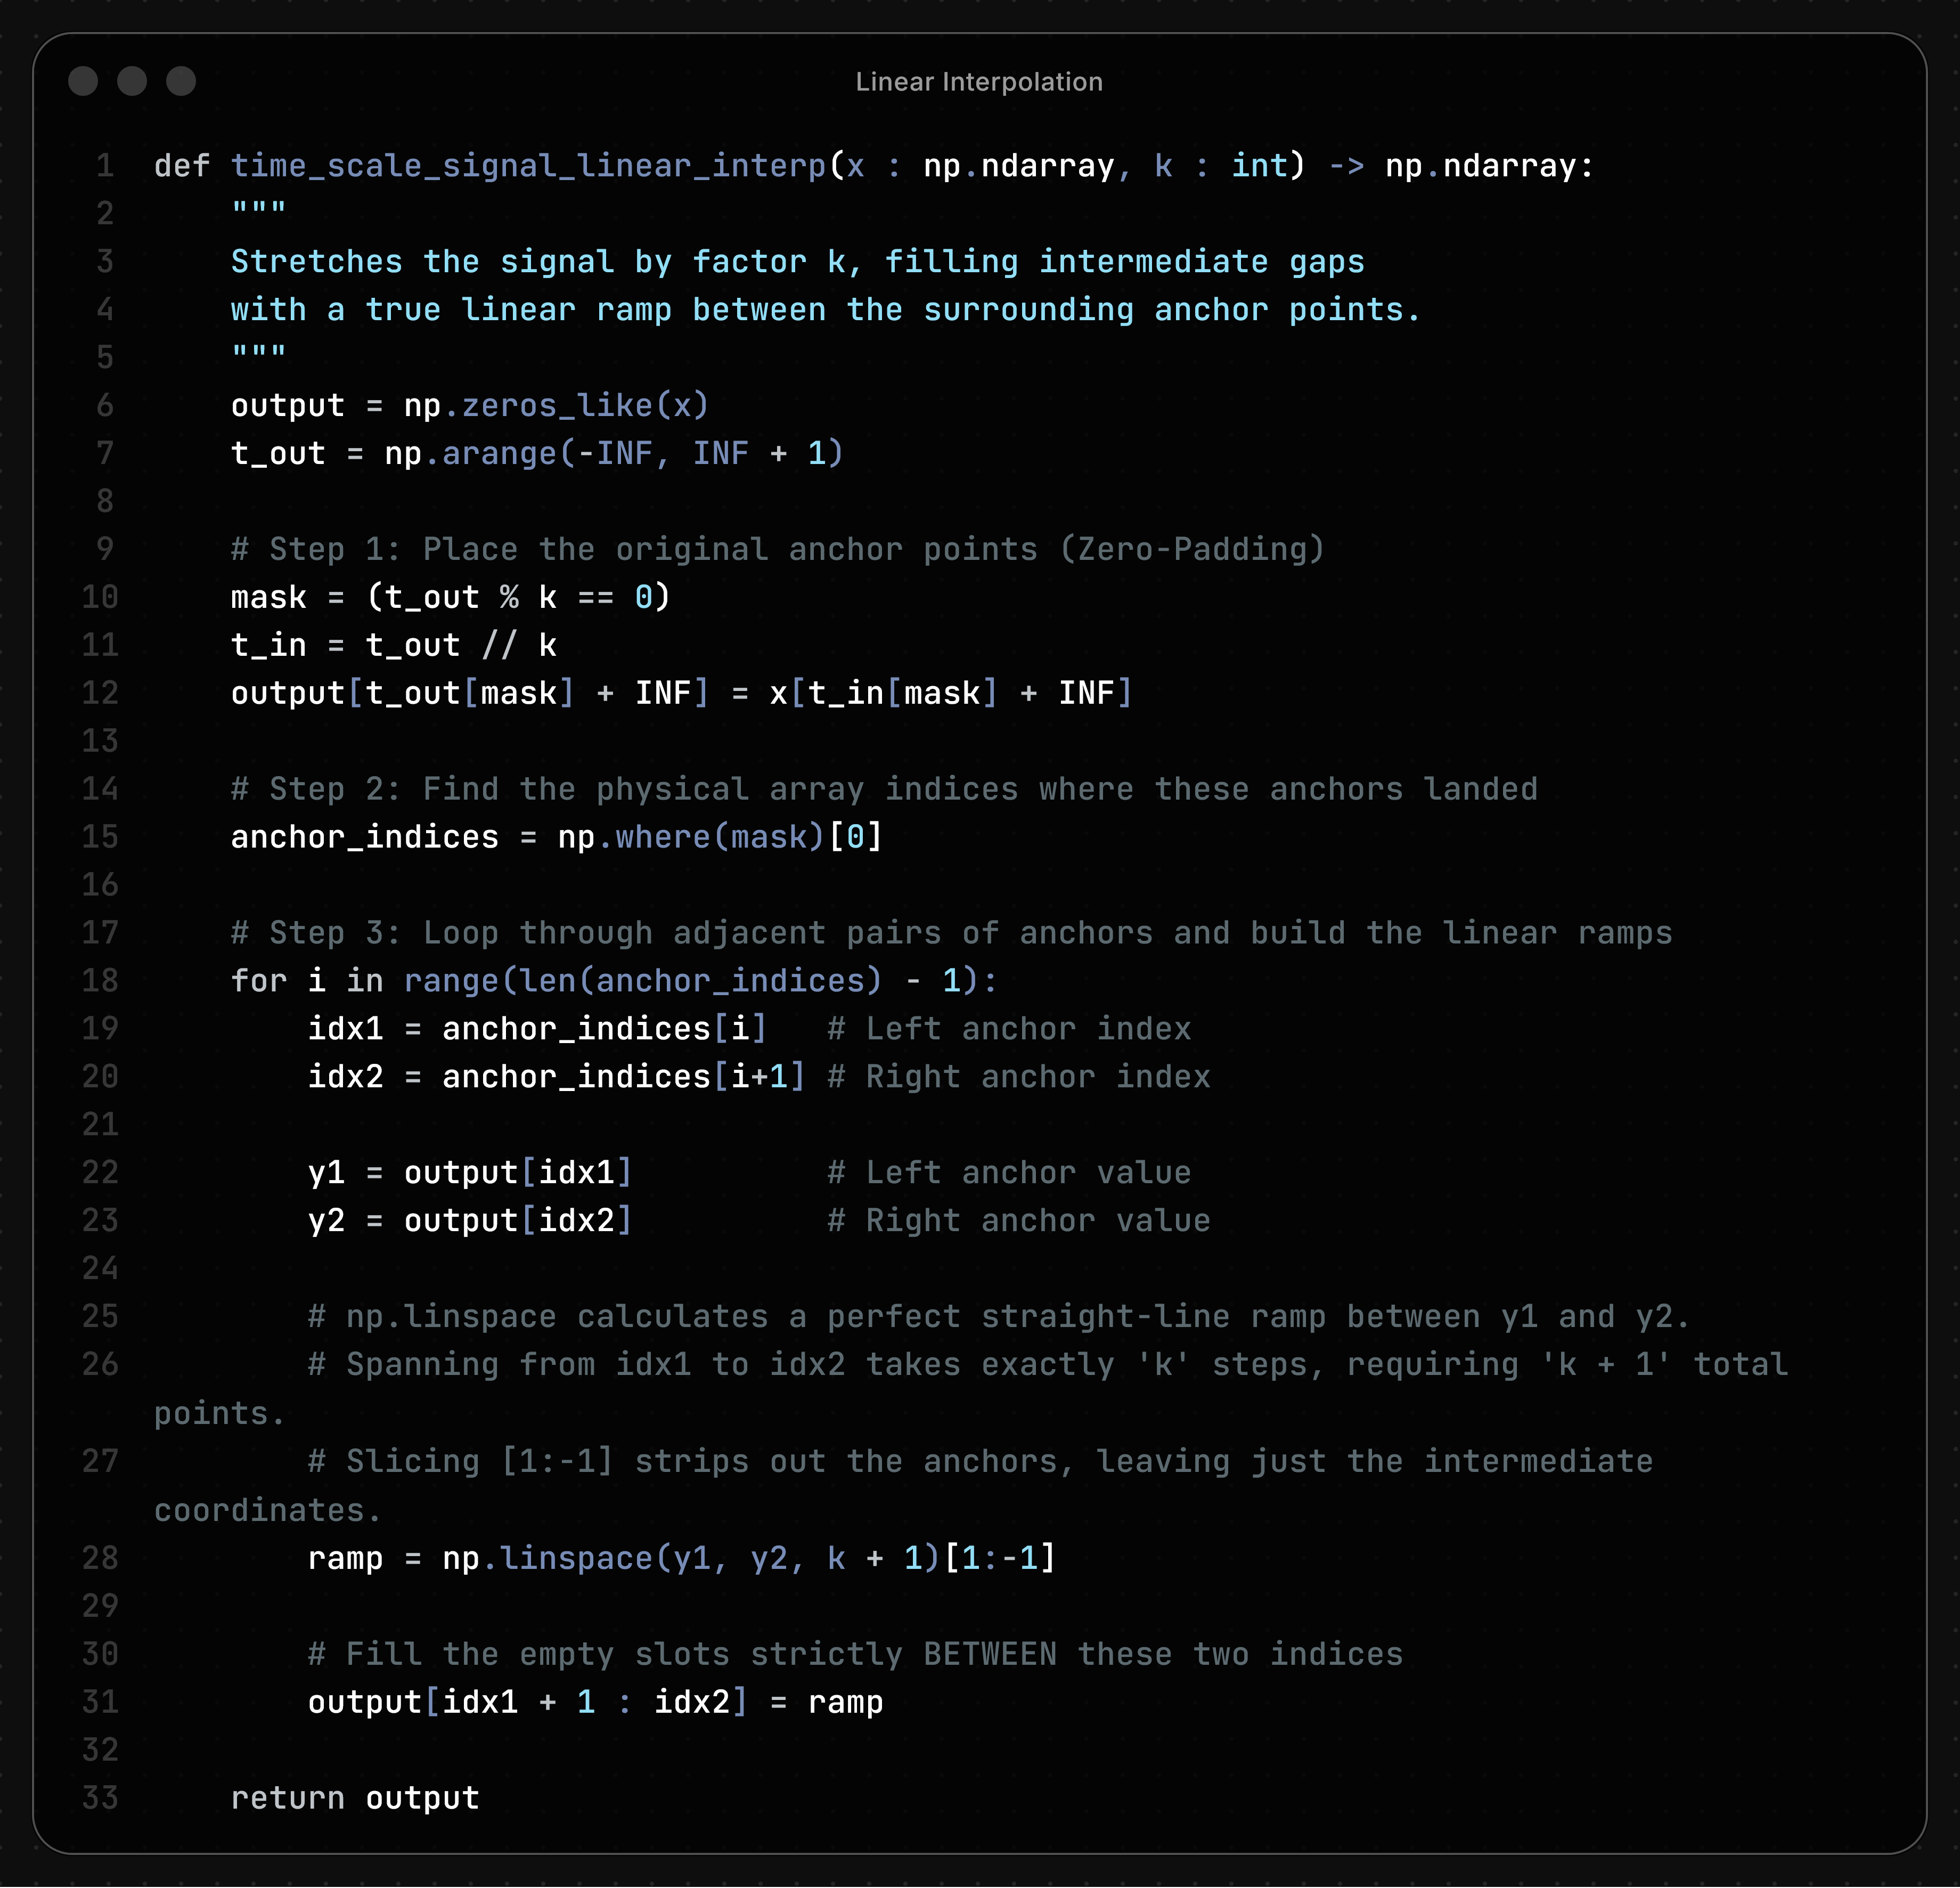
\includegraphics[width=\linewidth]{li.png}}
        \caption{Framed}
    \end{subfigure}\hfill
    \begin{subfigure}[b]{0.2\textwidth}
        \centering
        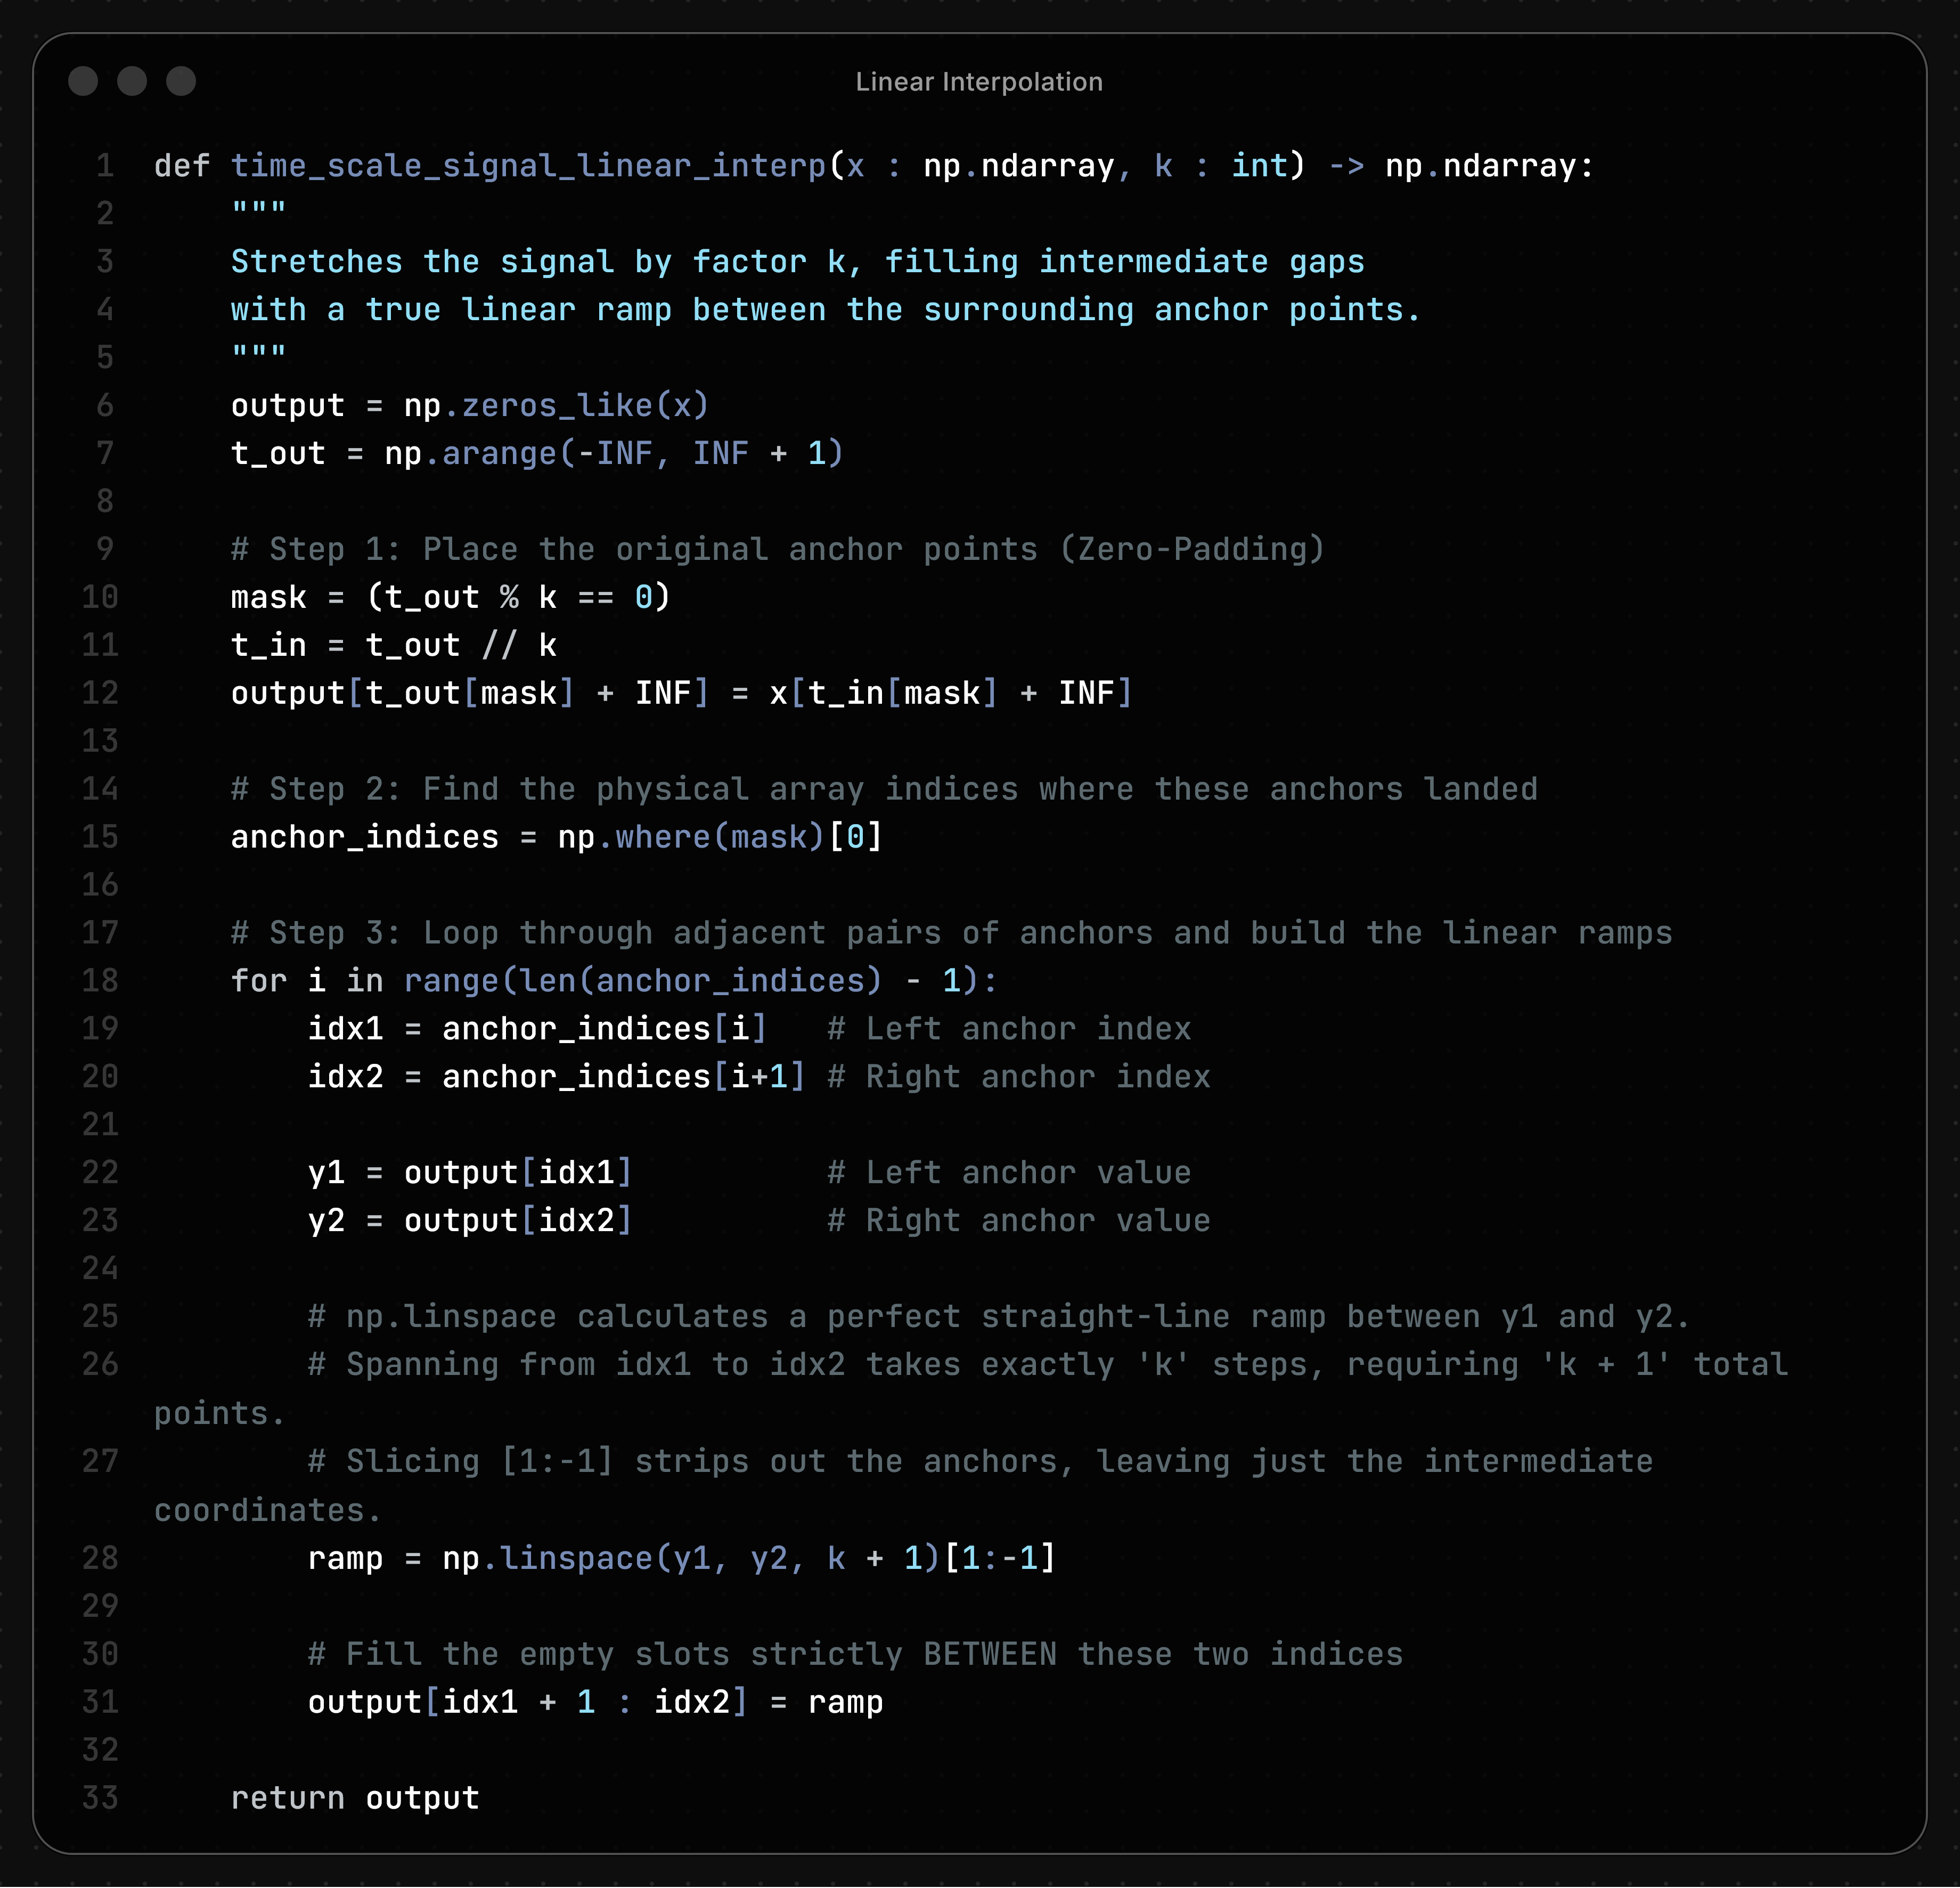
\includegraphics[height=2.2cm, keepaspectratio]{li.png}
        \caption{Fixed height}
    \end{subfigure}\hfill
    \begin{subfigure}[b]{0.2\textwidth}
        \centering
        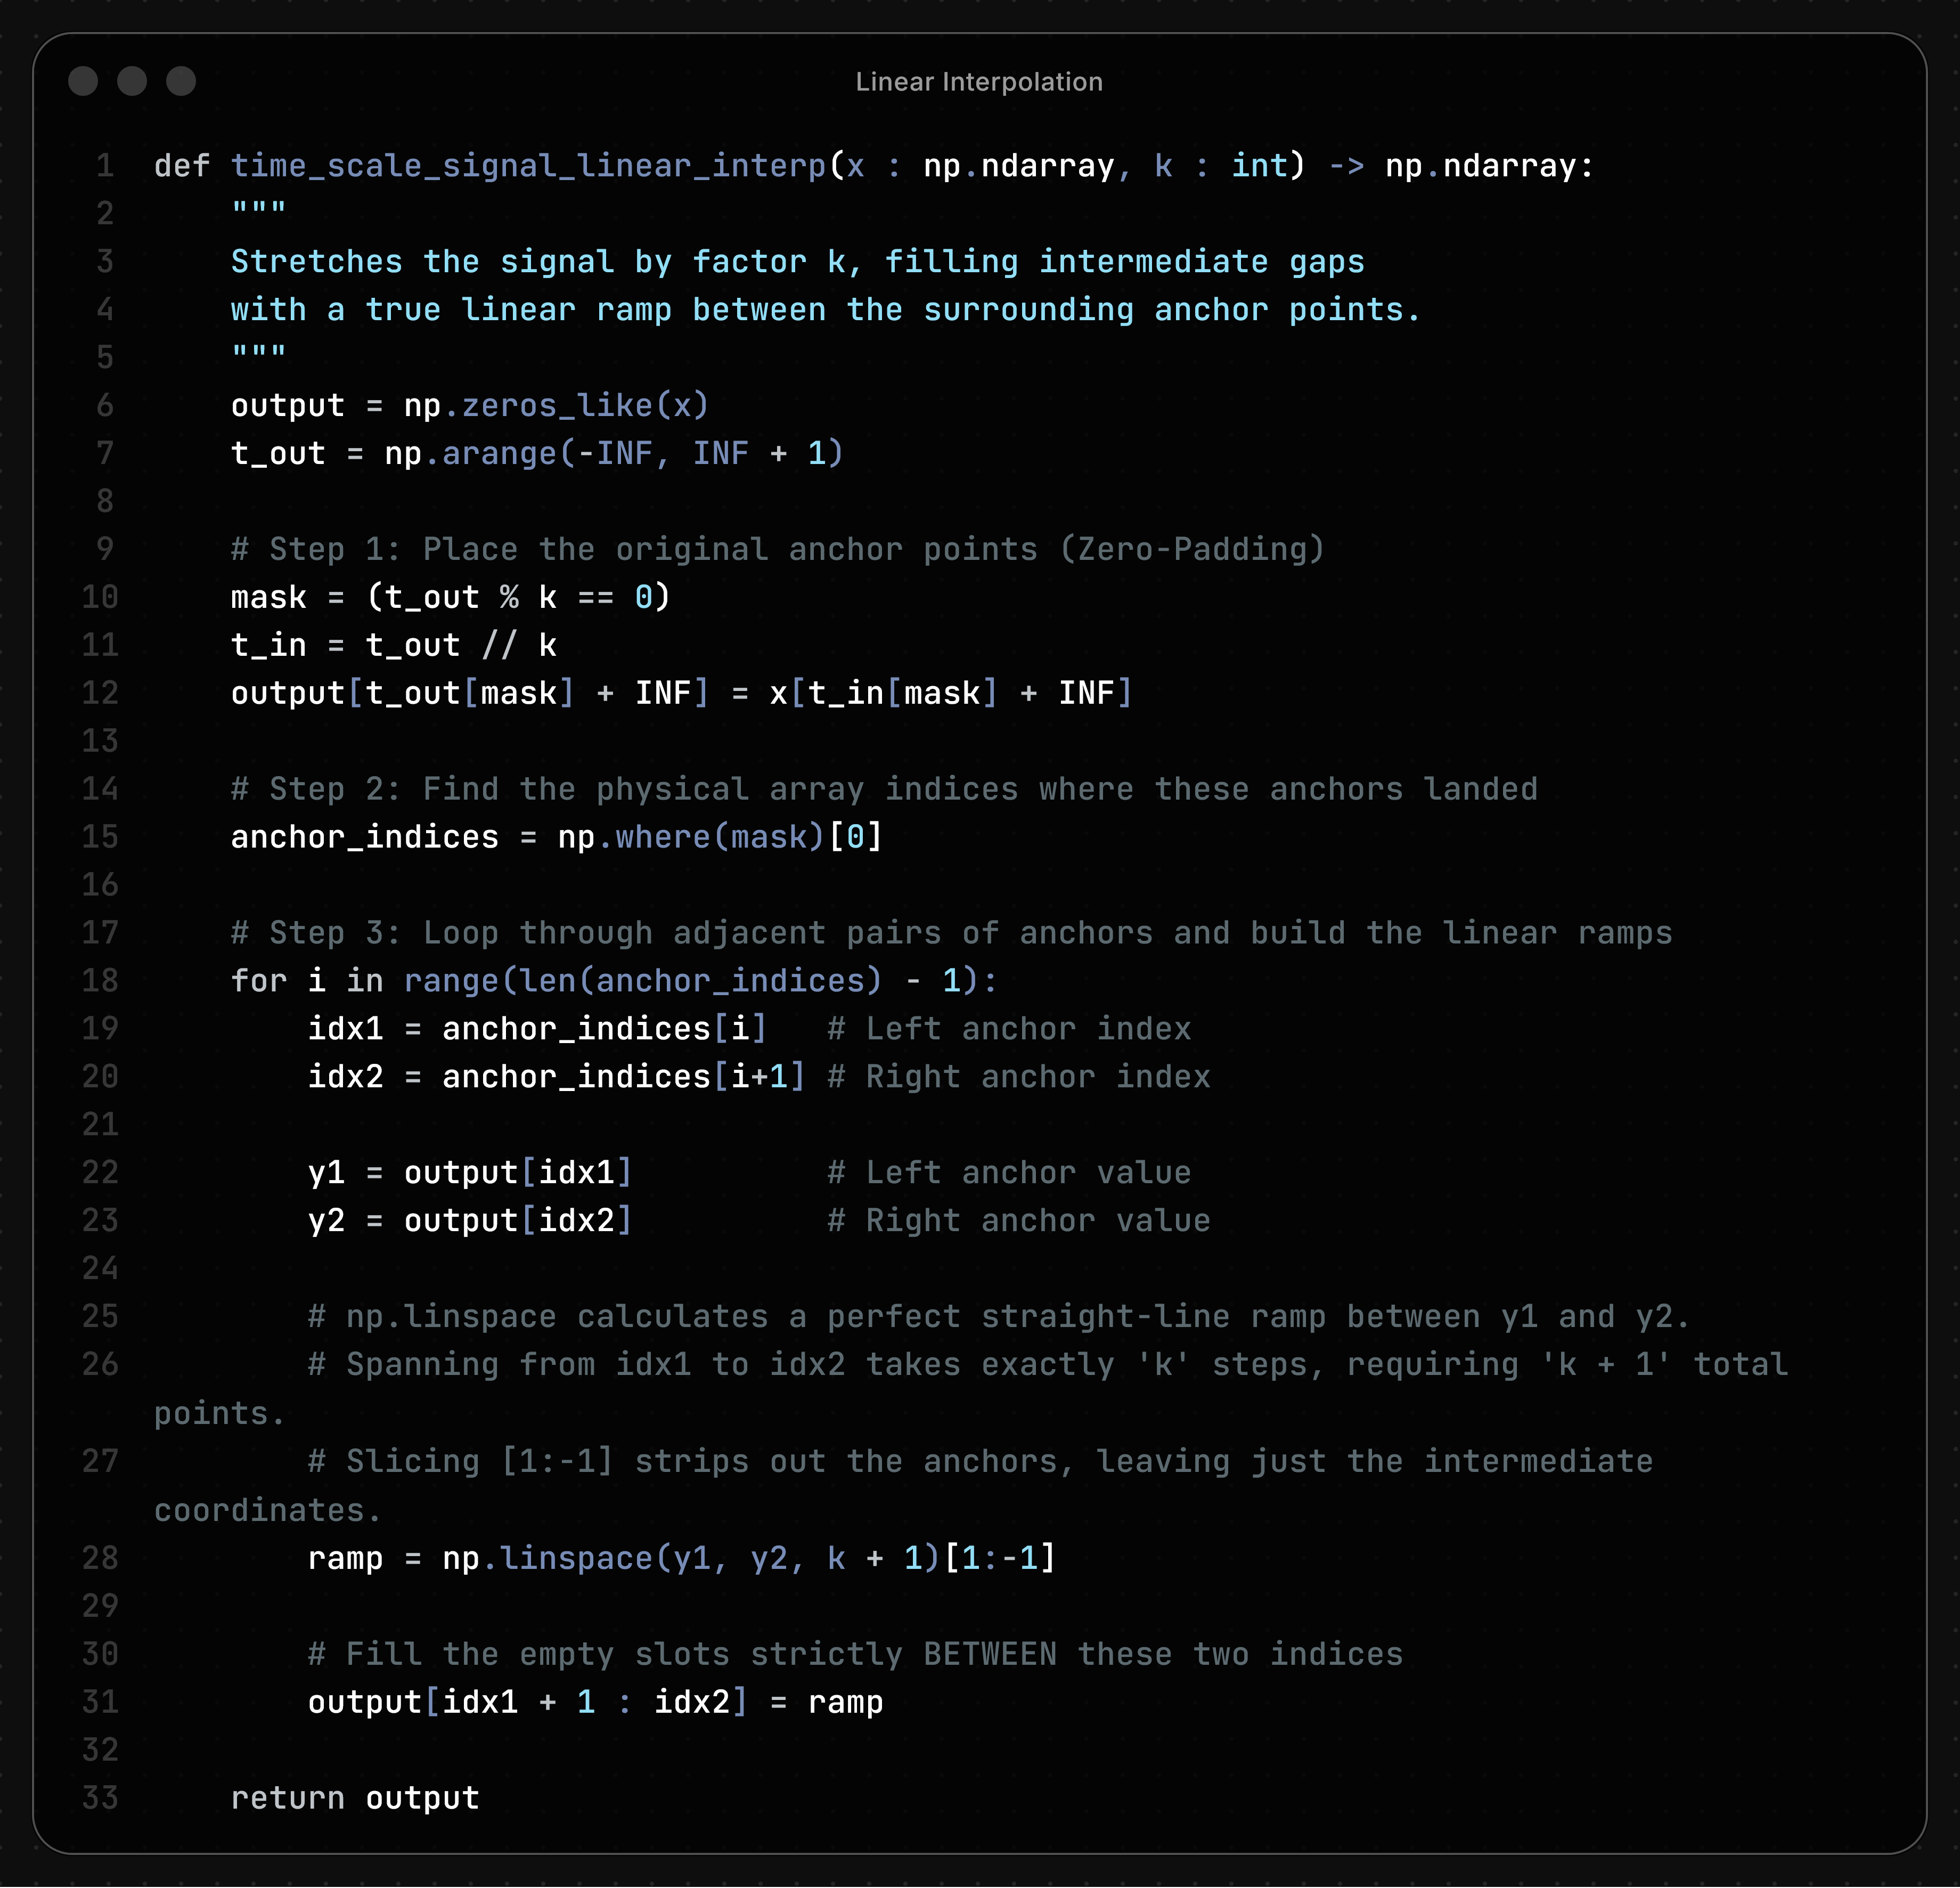
\includegraphics[width=\linewidth, trim=2cm 1cm 2cm 1cm, clip]{li.png}
        \caption{Cropped}
    \end{subfigure}\hfill
    \begin{subfigure}[b]{0.2\textwidth}
        \centering
        \resizebox{\linewidth}{2.2cm}{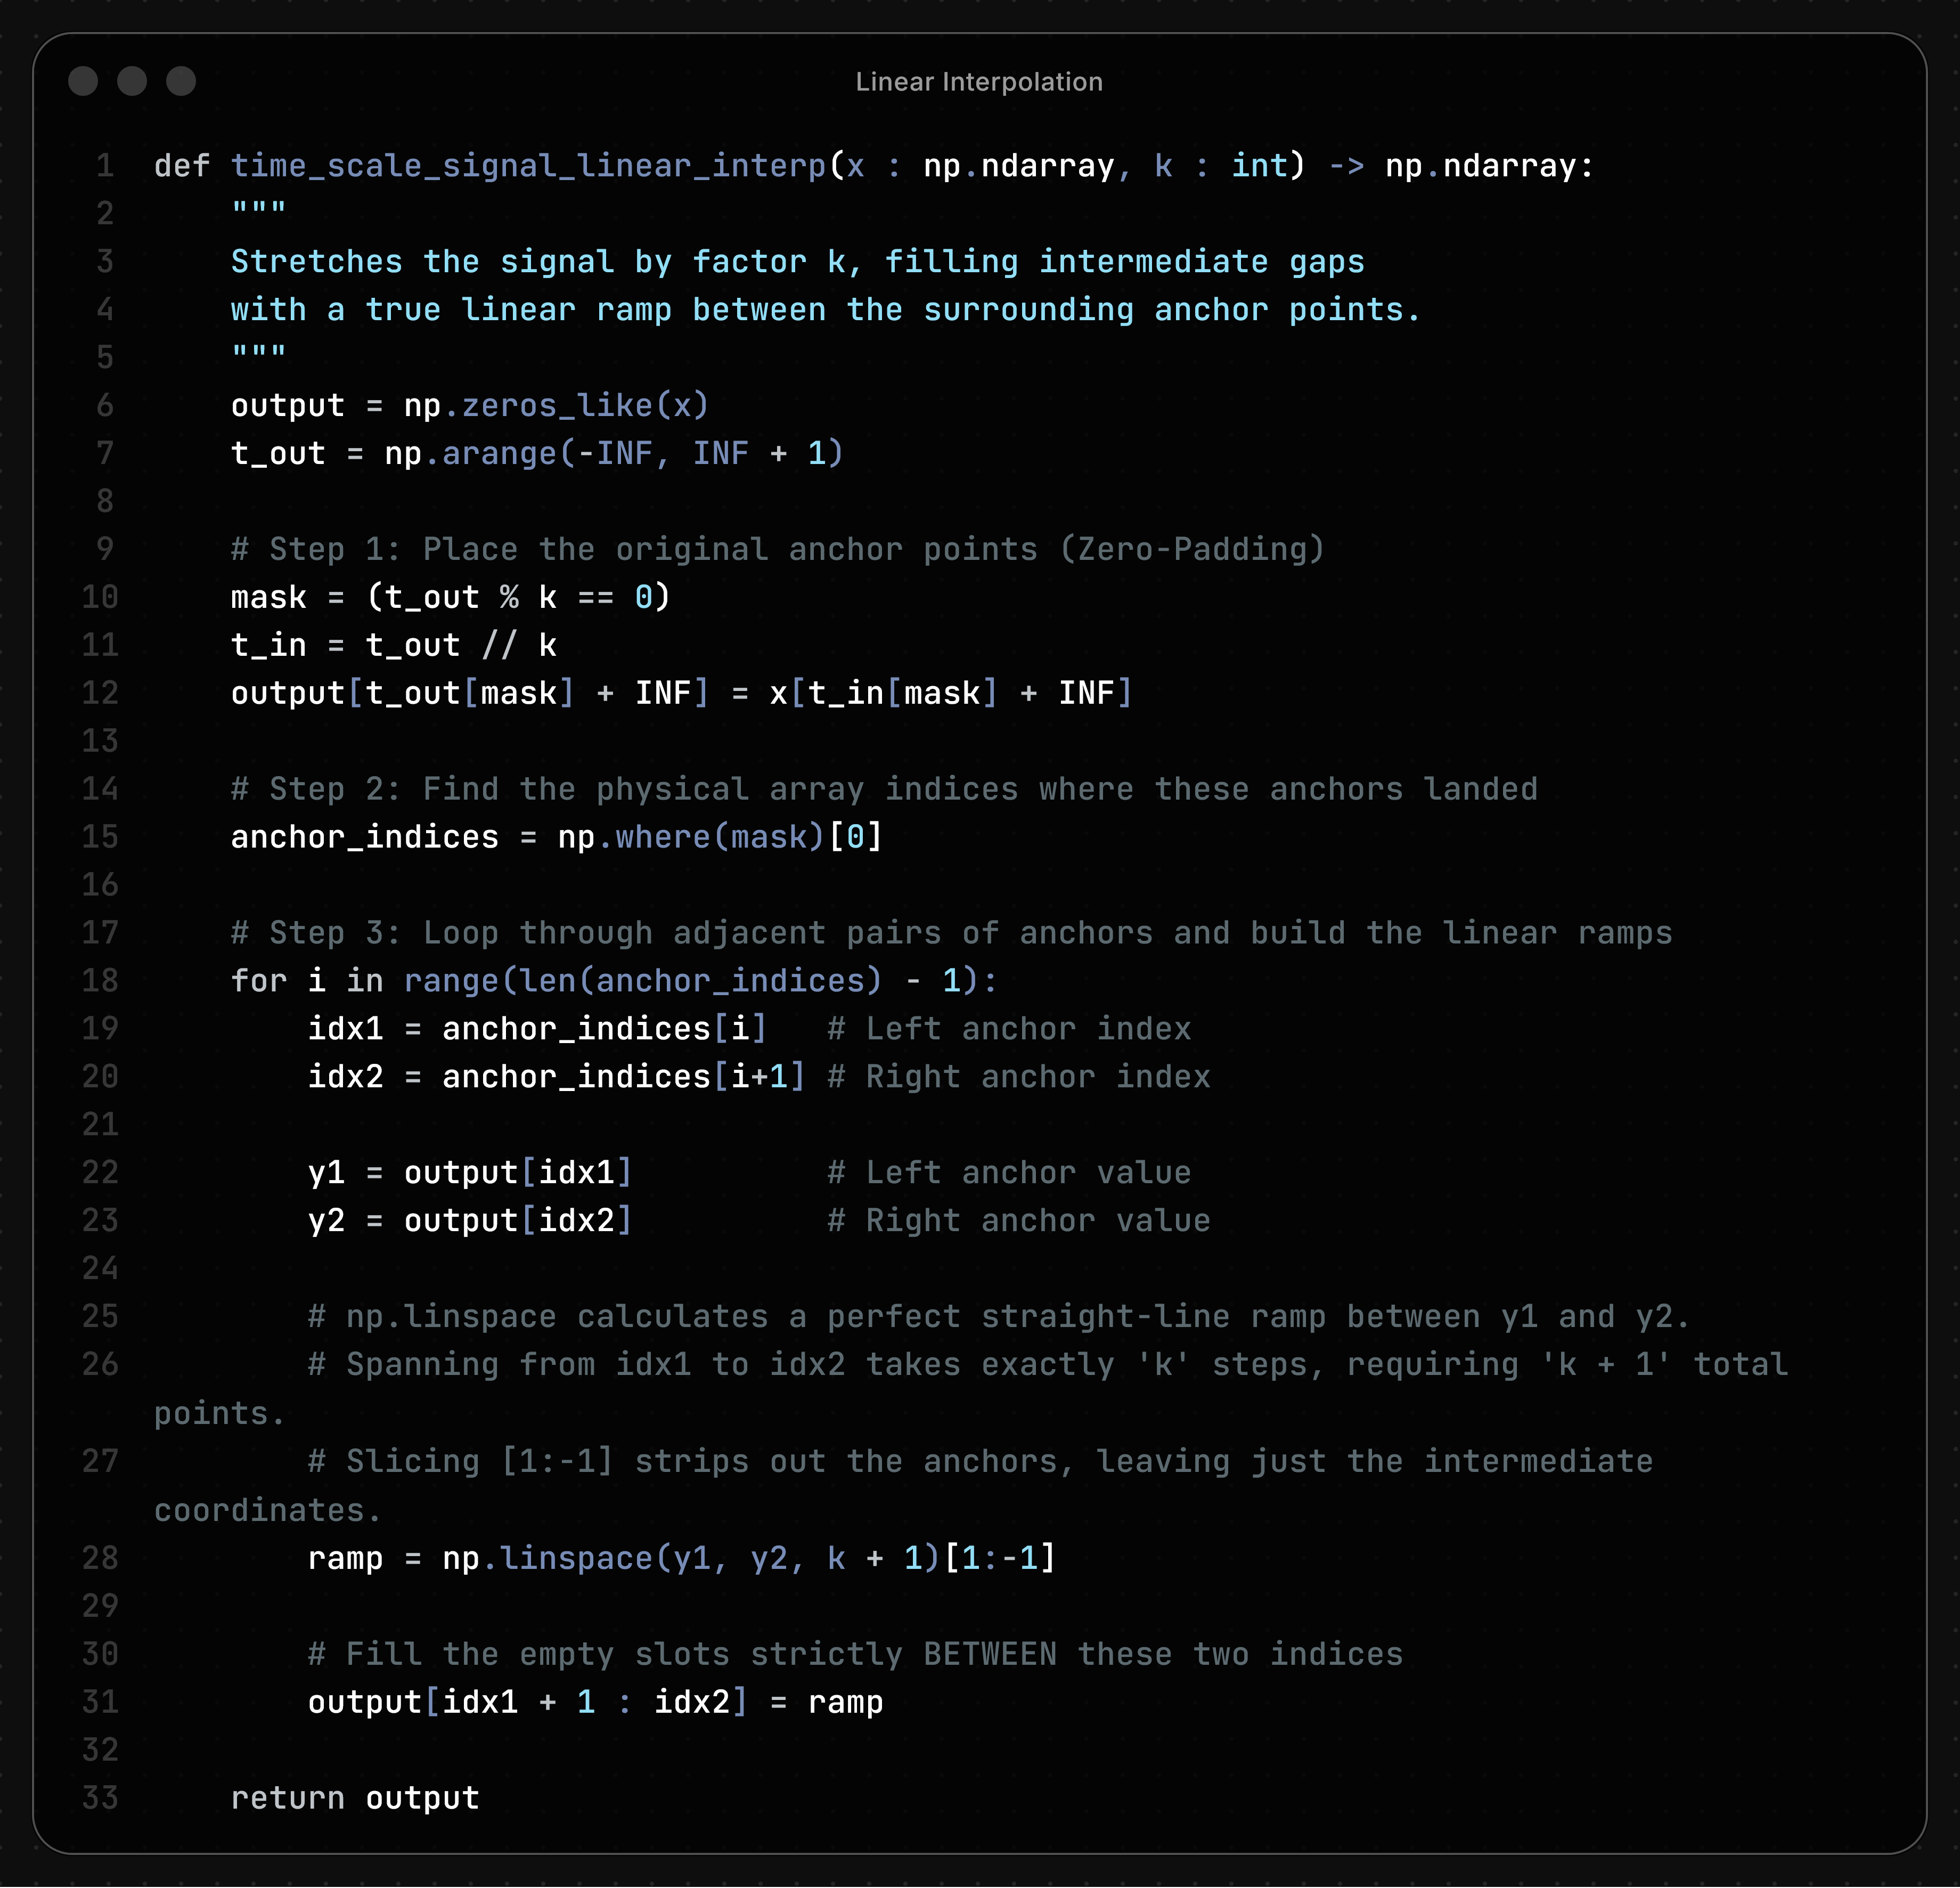
\includegraphics{li.png}}
        \caption{Stretched}
    \end{subfigure}
    
    \caption{Four ways to control the size and extent of an image.}
    \label{fig:image_control}
\end{figure}


% \fbox{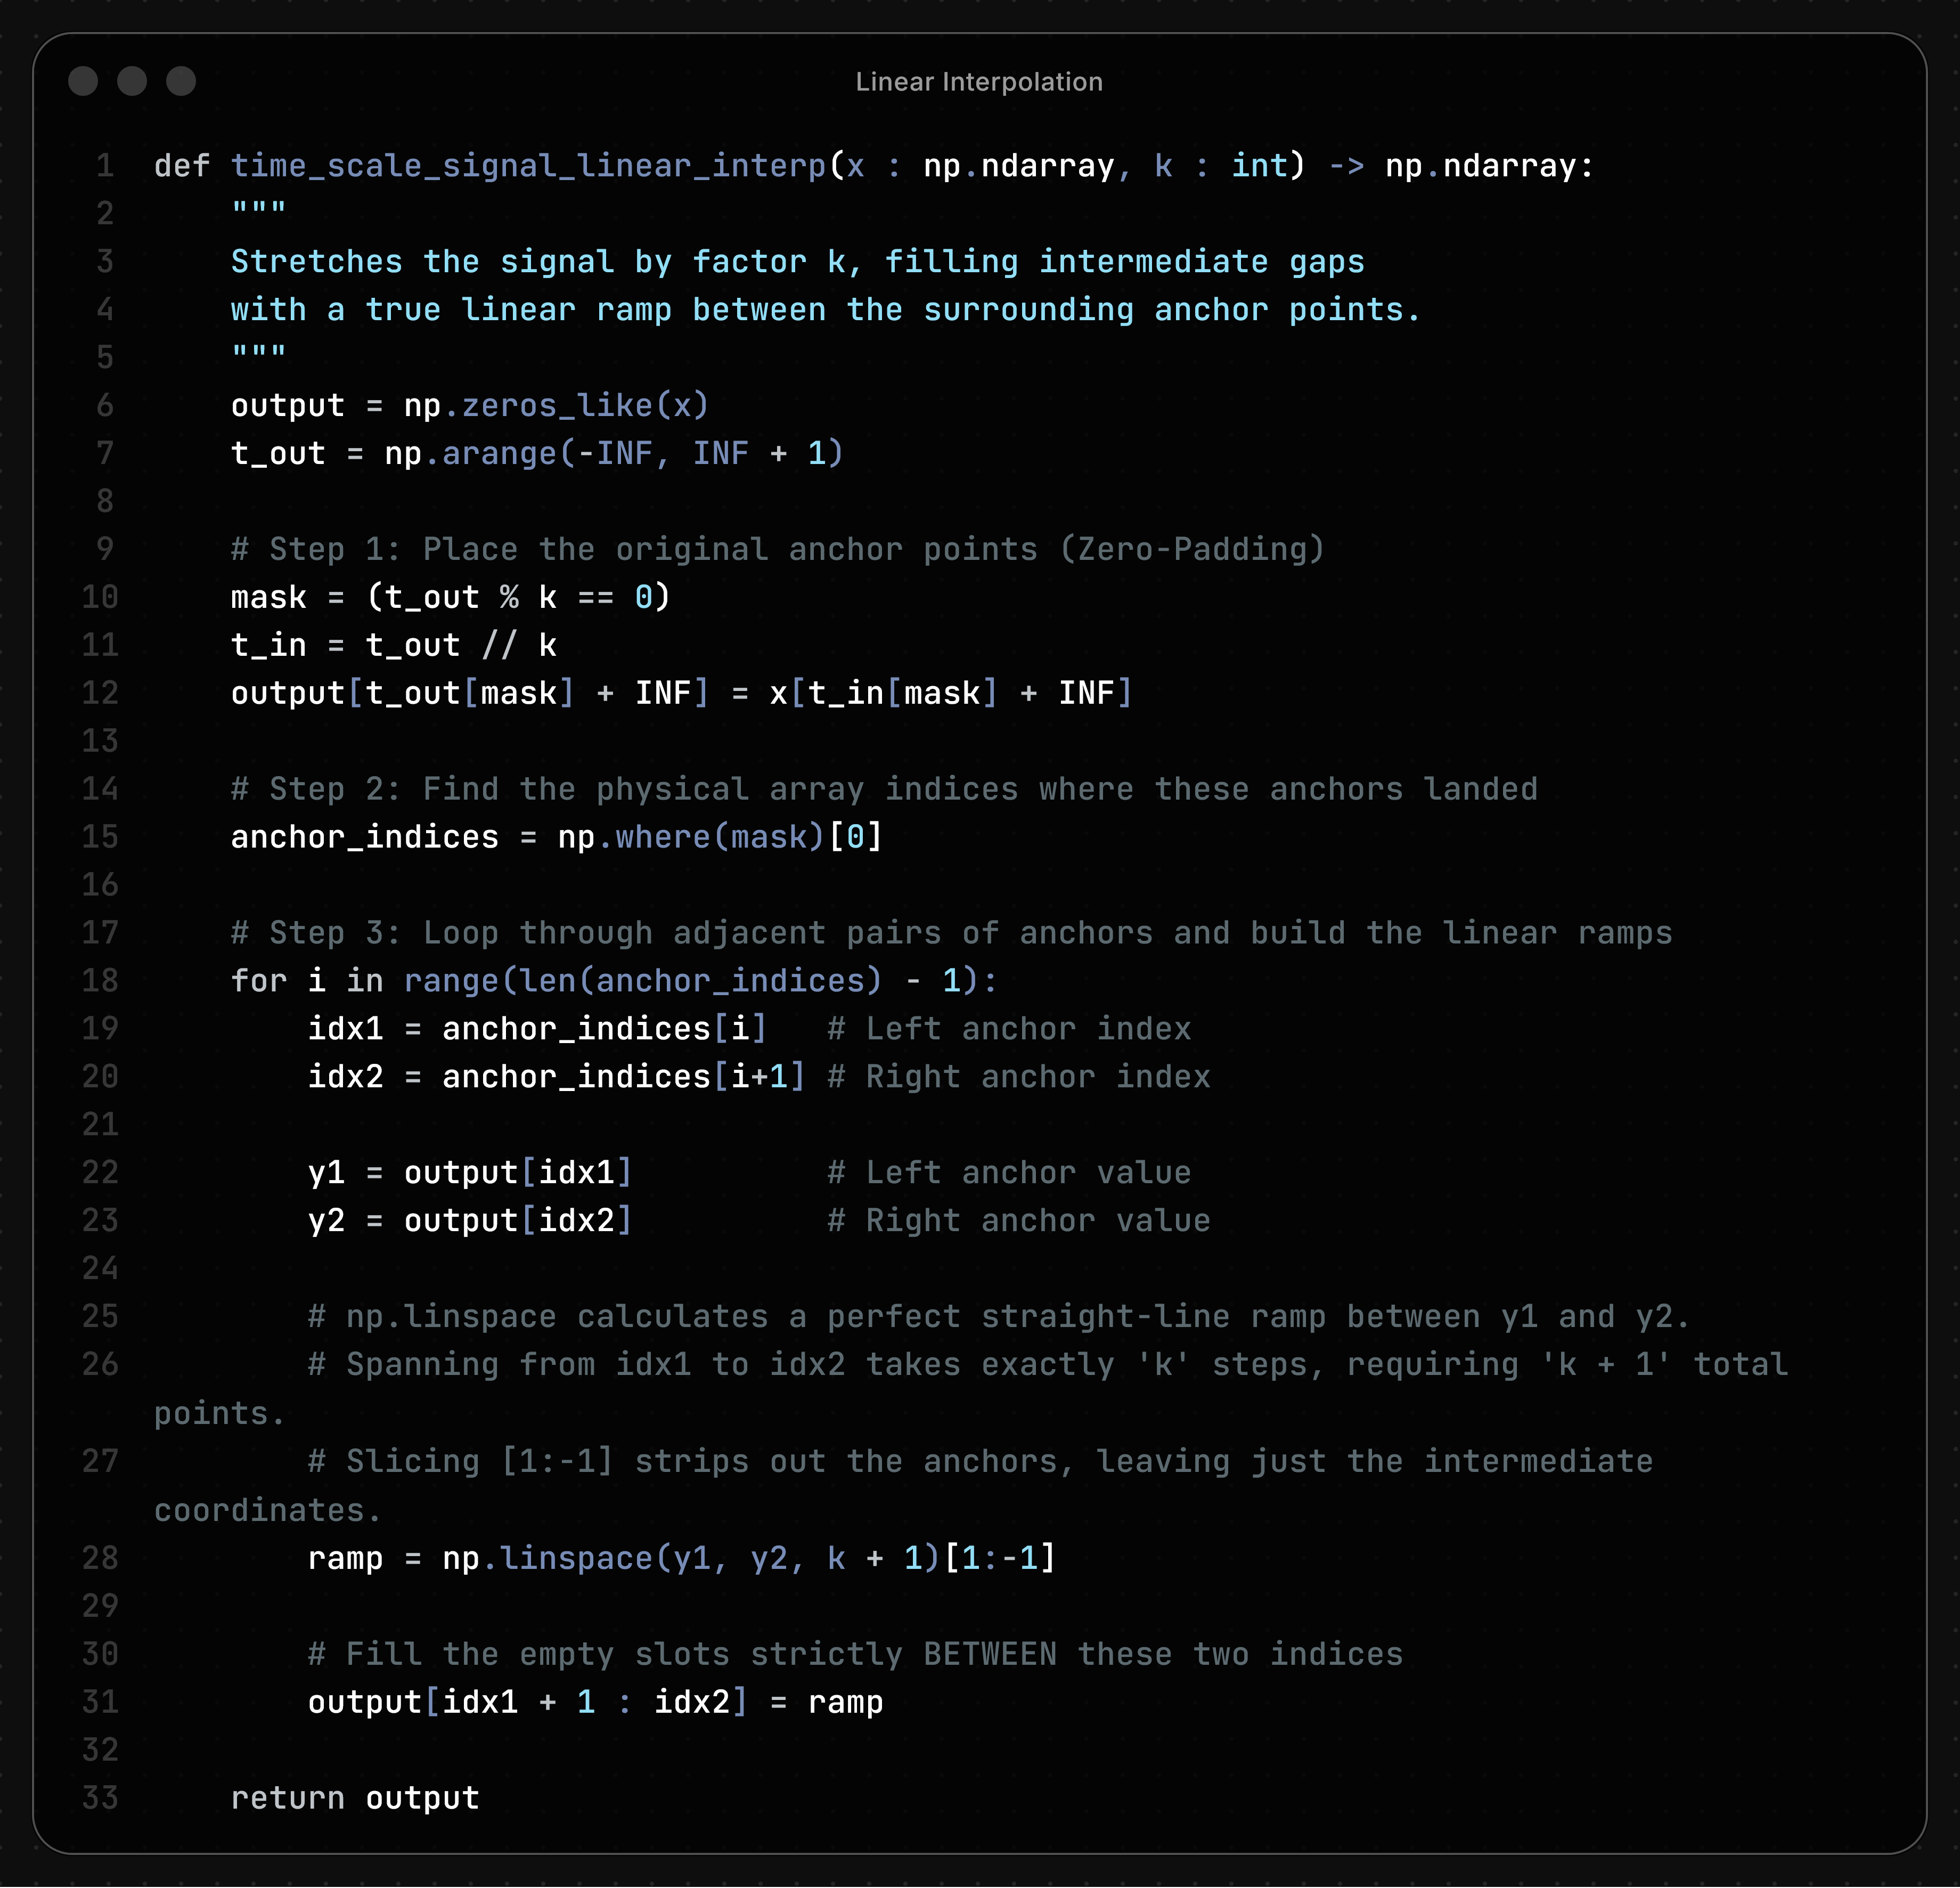
\includegraphics[width=\linewidth]{li.png}} % framed
% 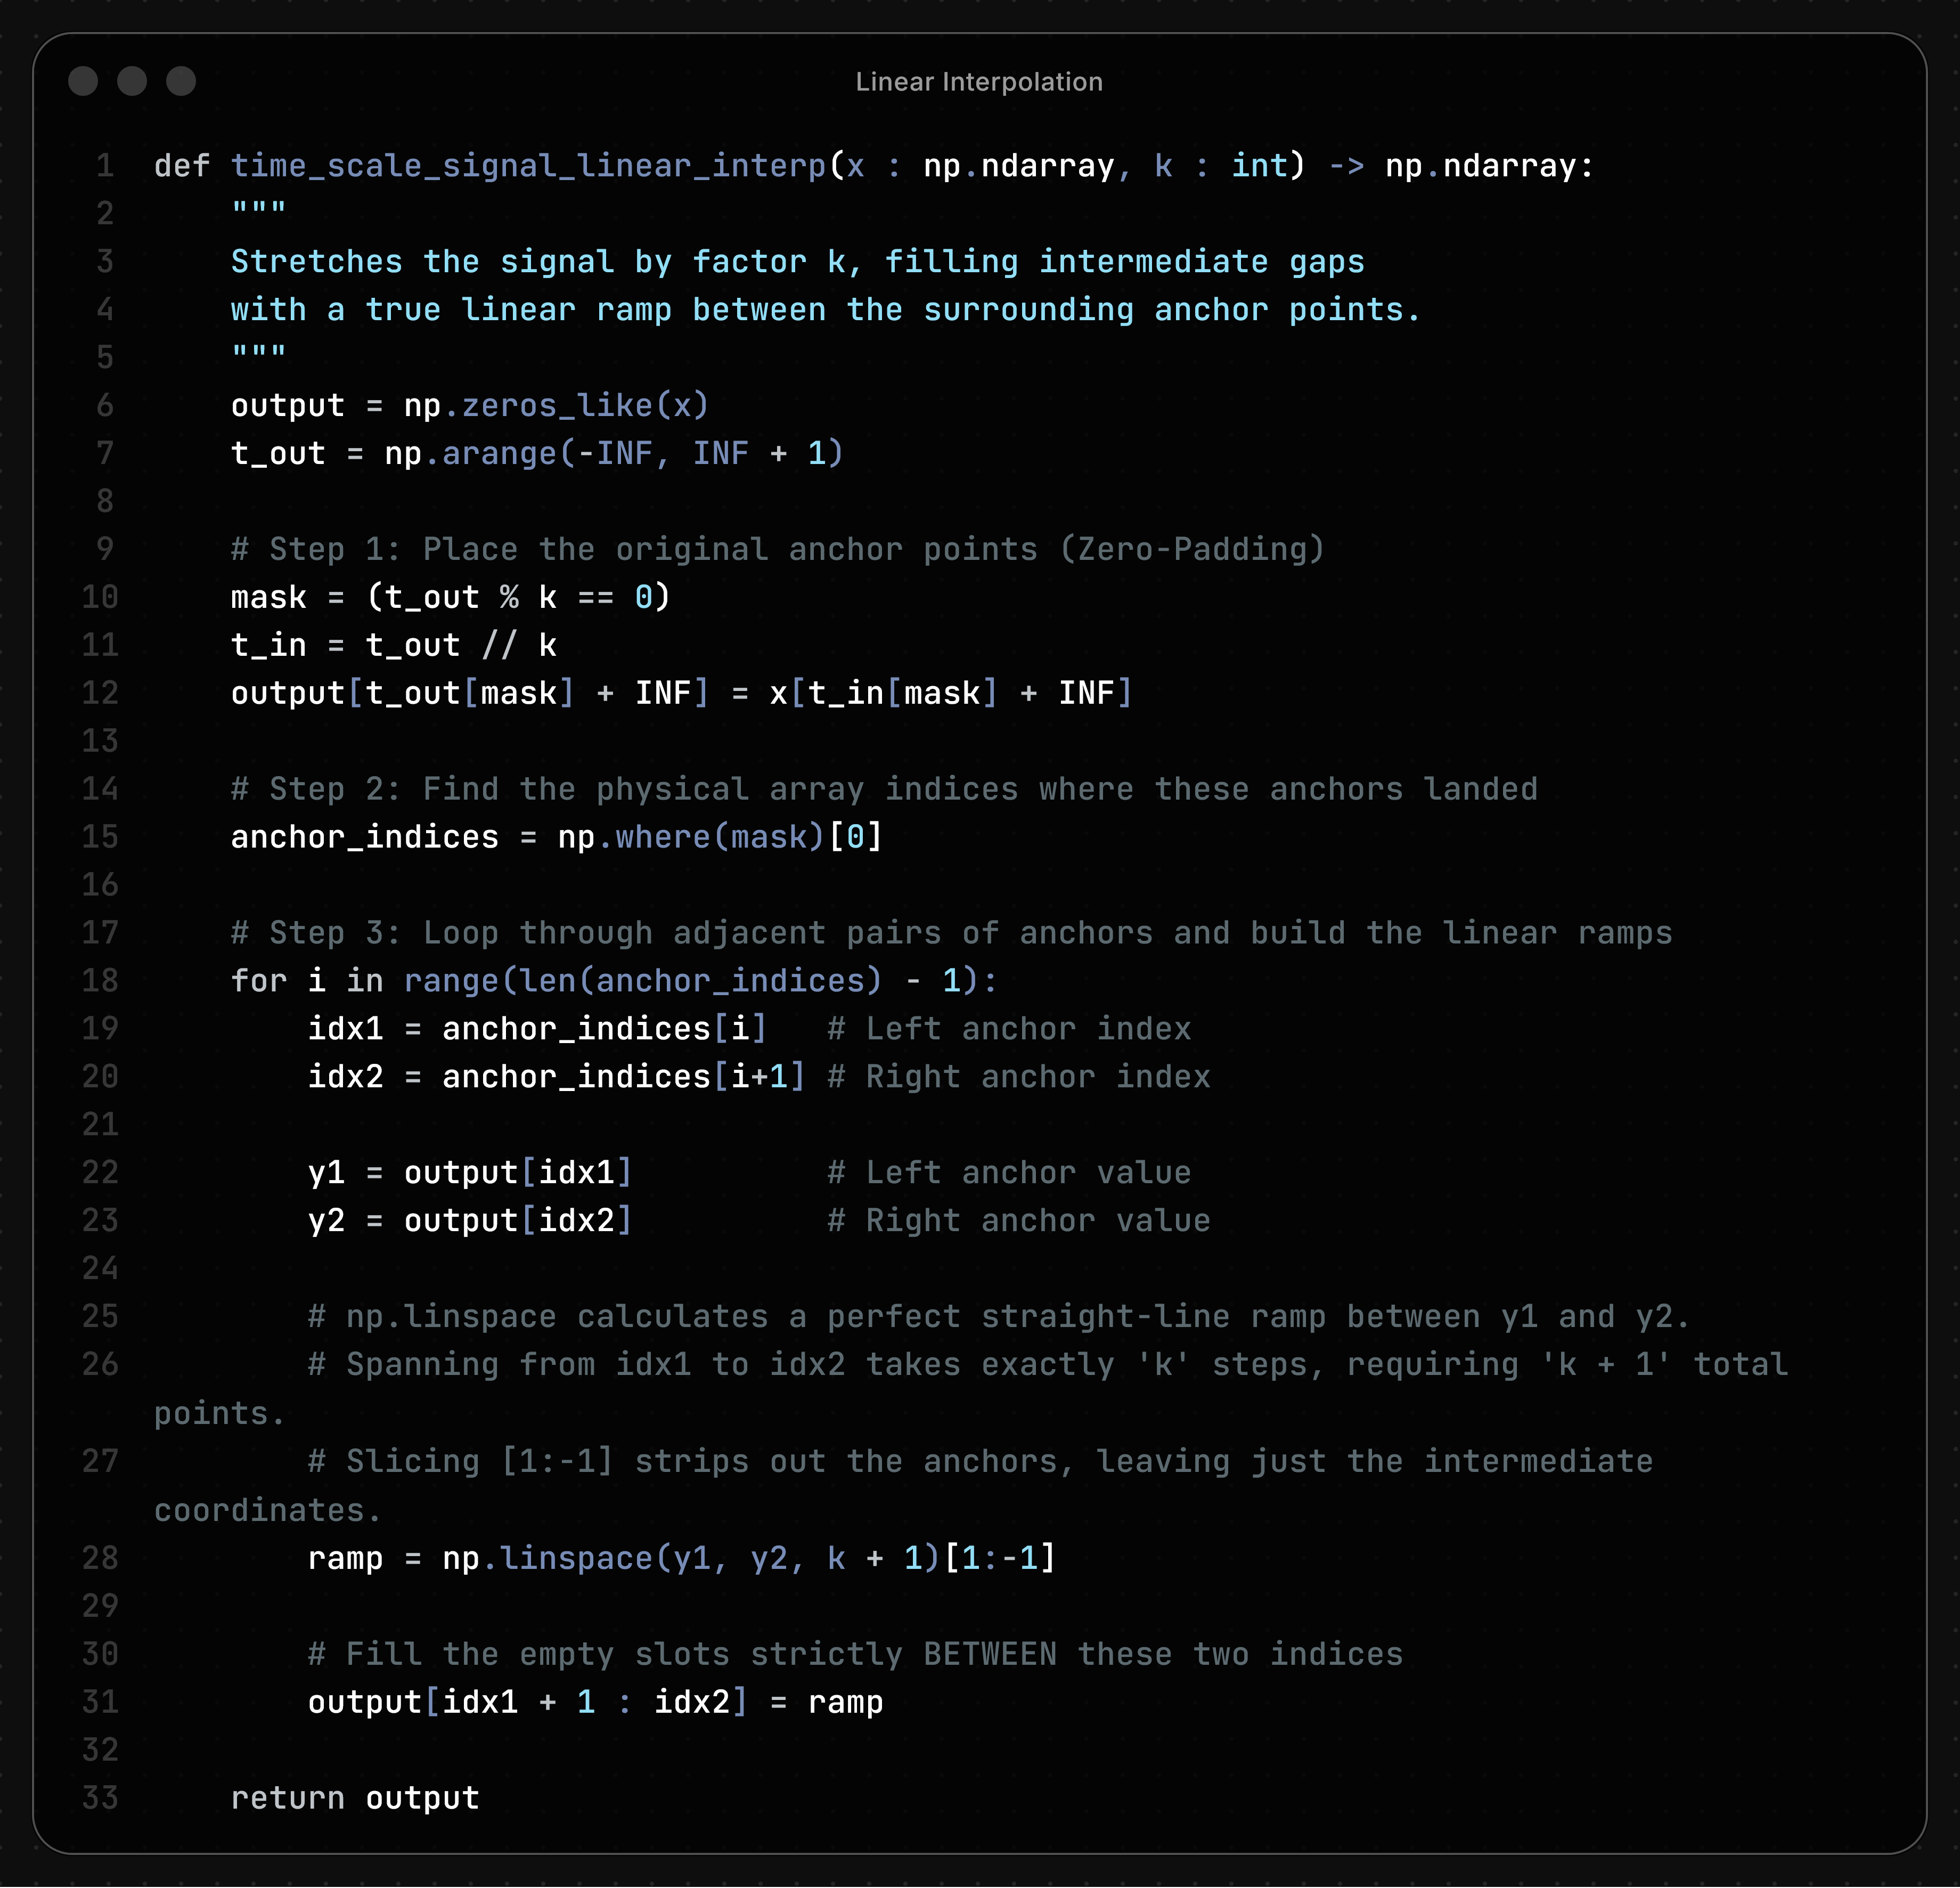
\includegraphics[height=2.2cm, keepaspectratio]{li.png} % fixed height
% 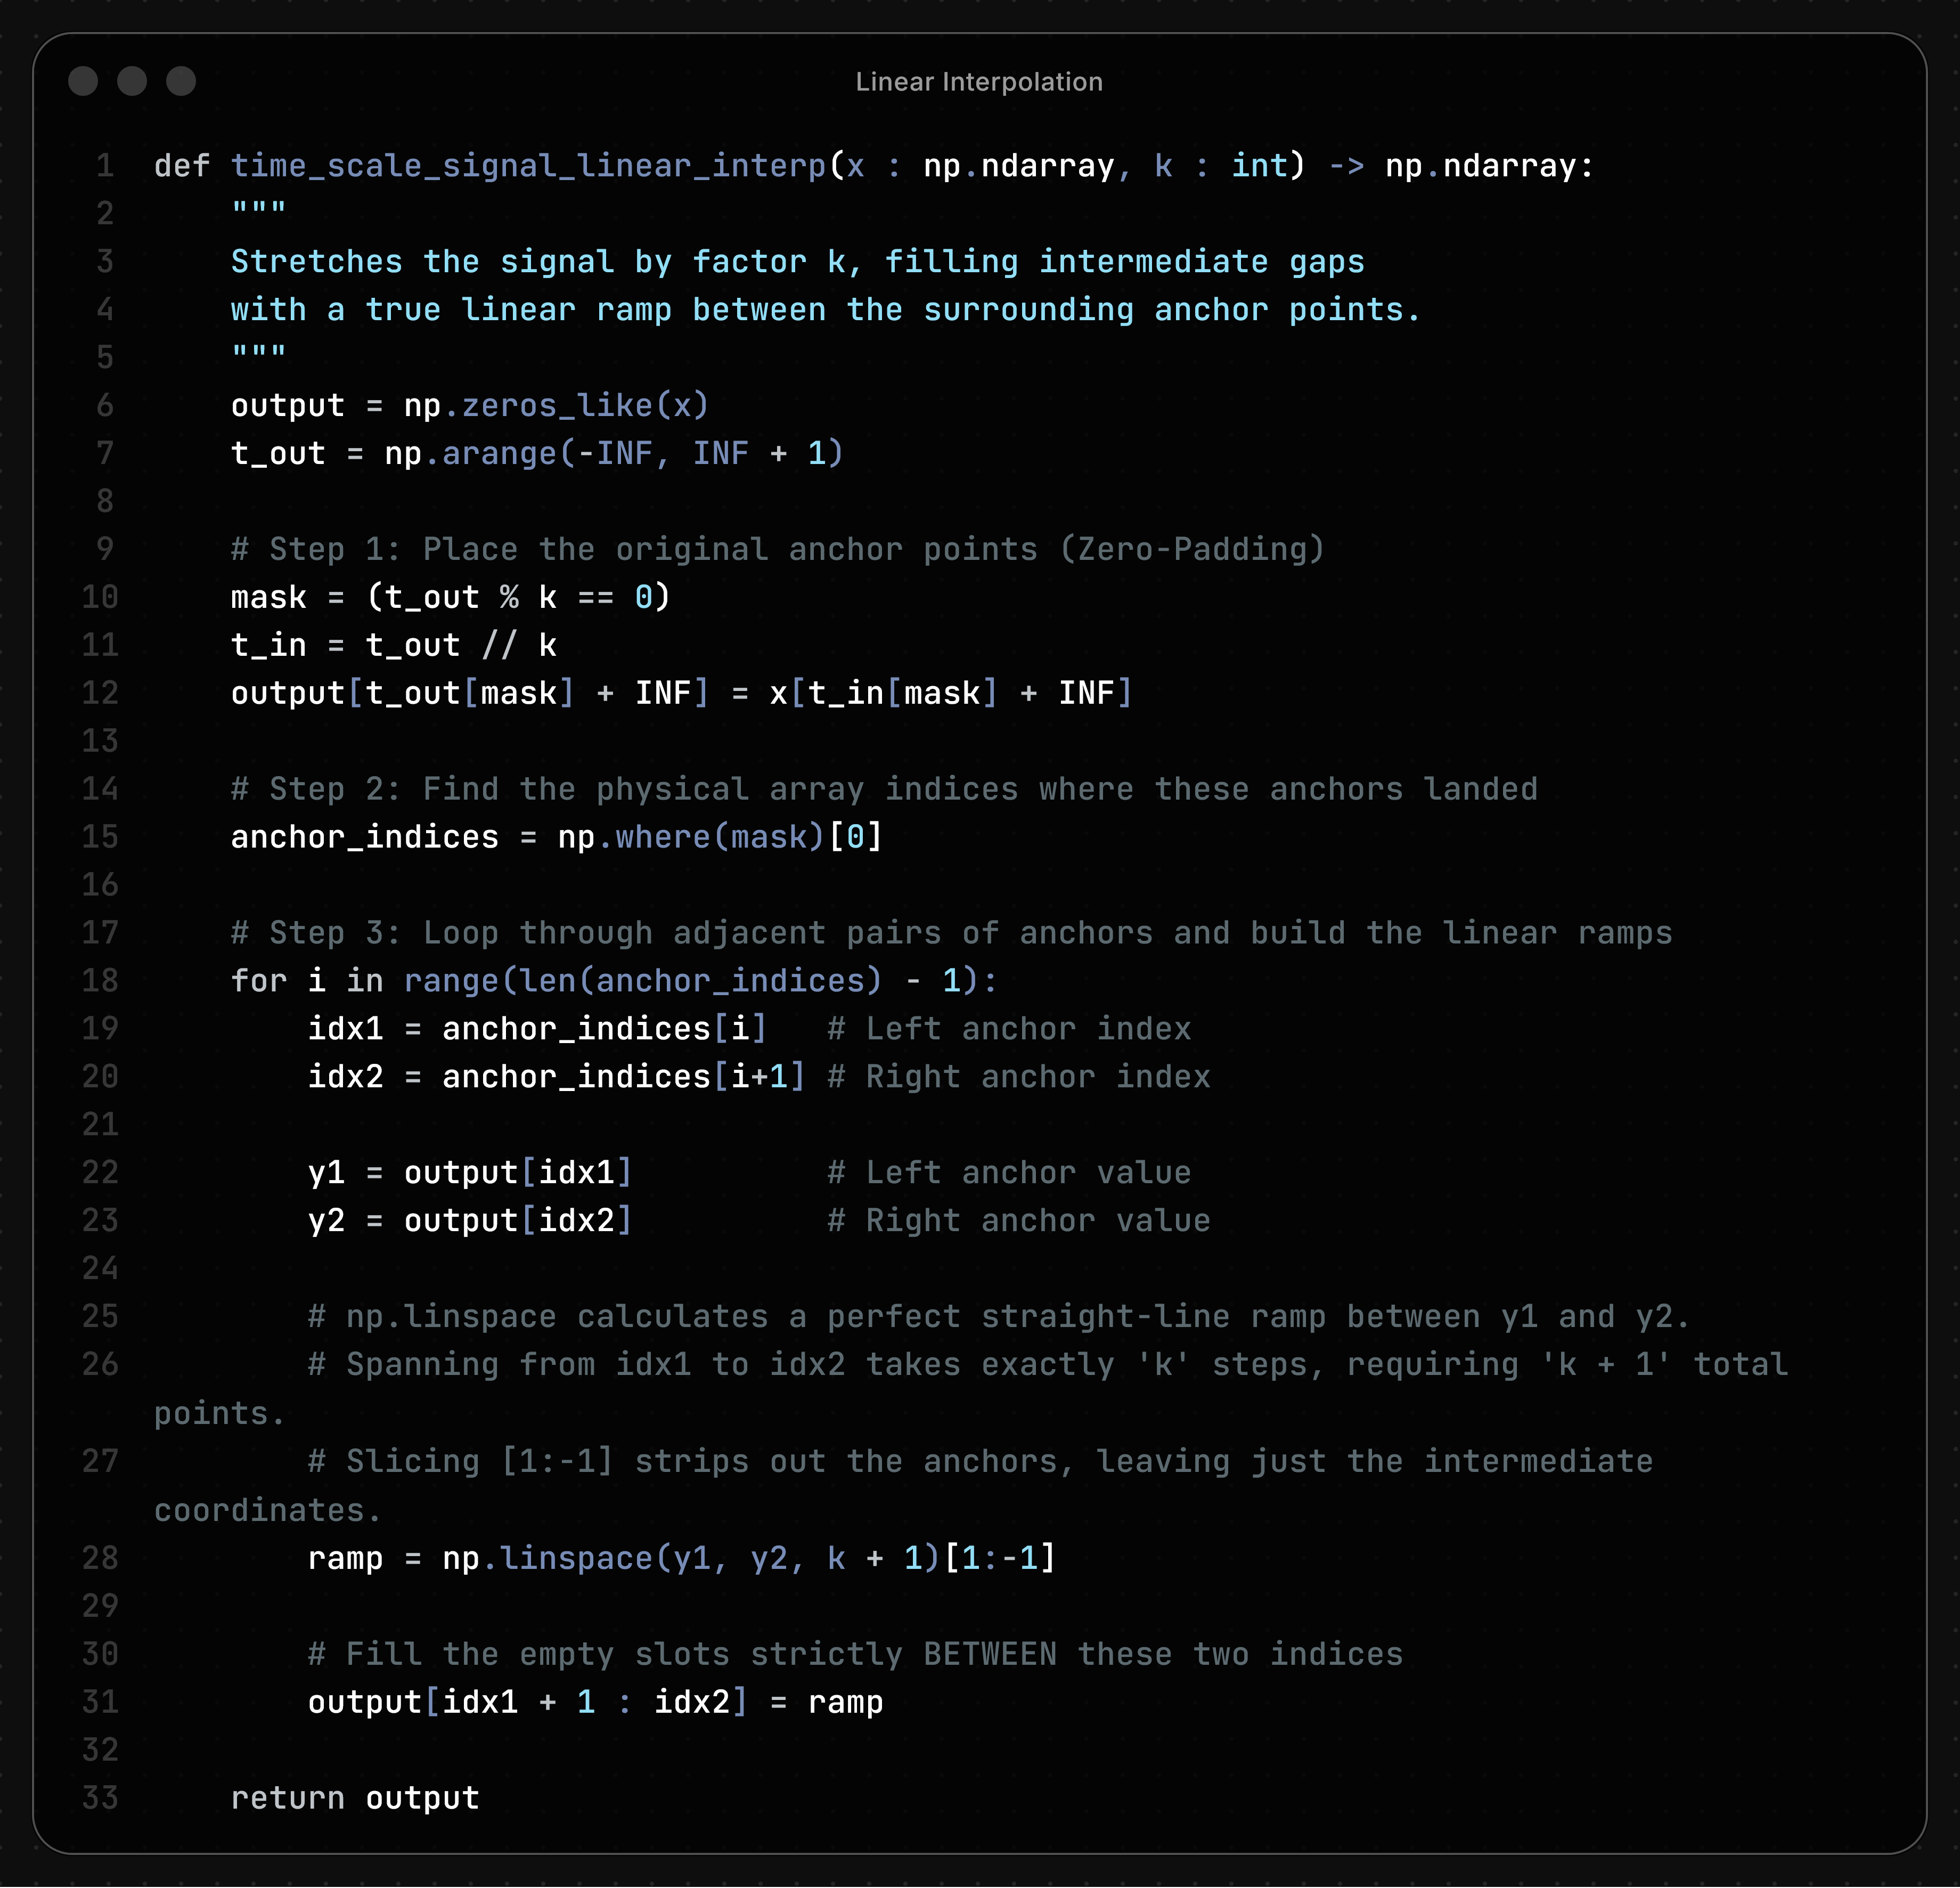
\includegraphics[width=\linewidth, trim=2cm 1cm 2cm 1cm, clip]{li.png}
% \resizebox{\linewidth}{2.2cm}{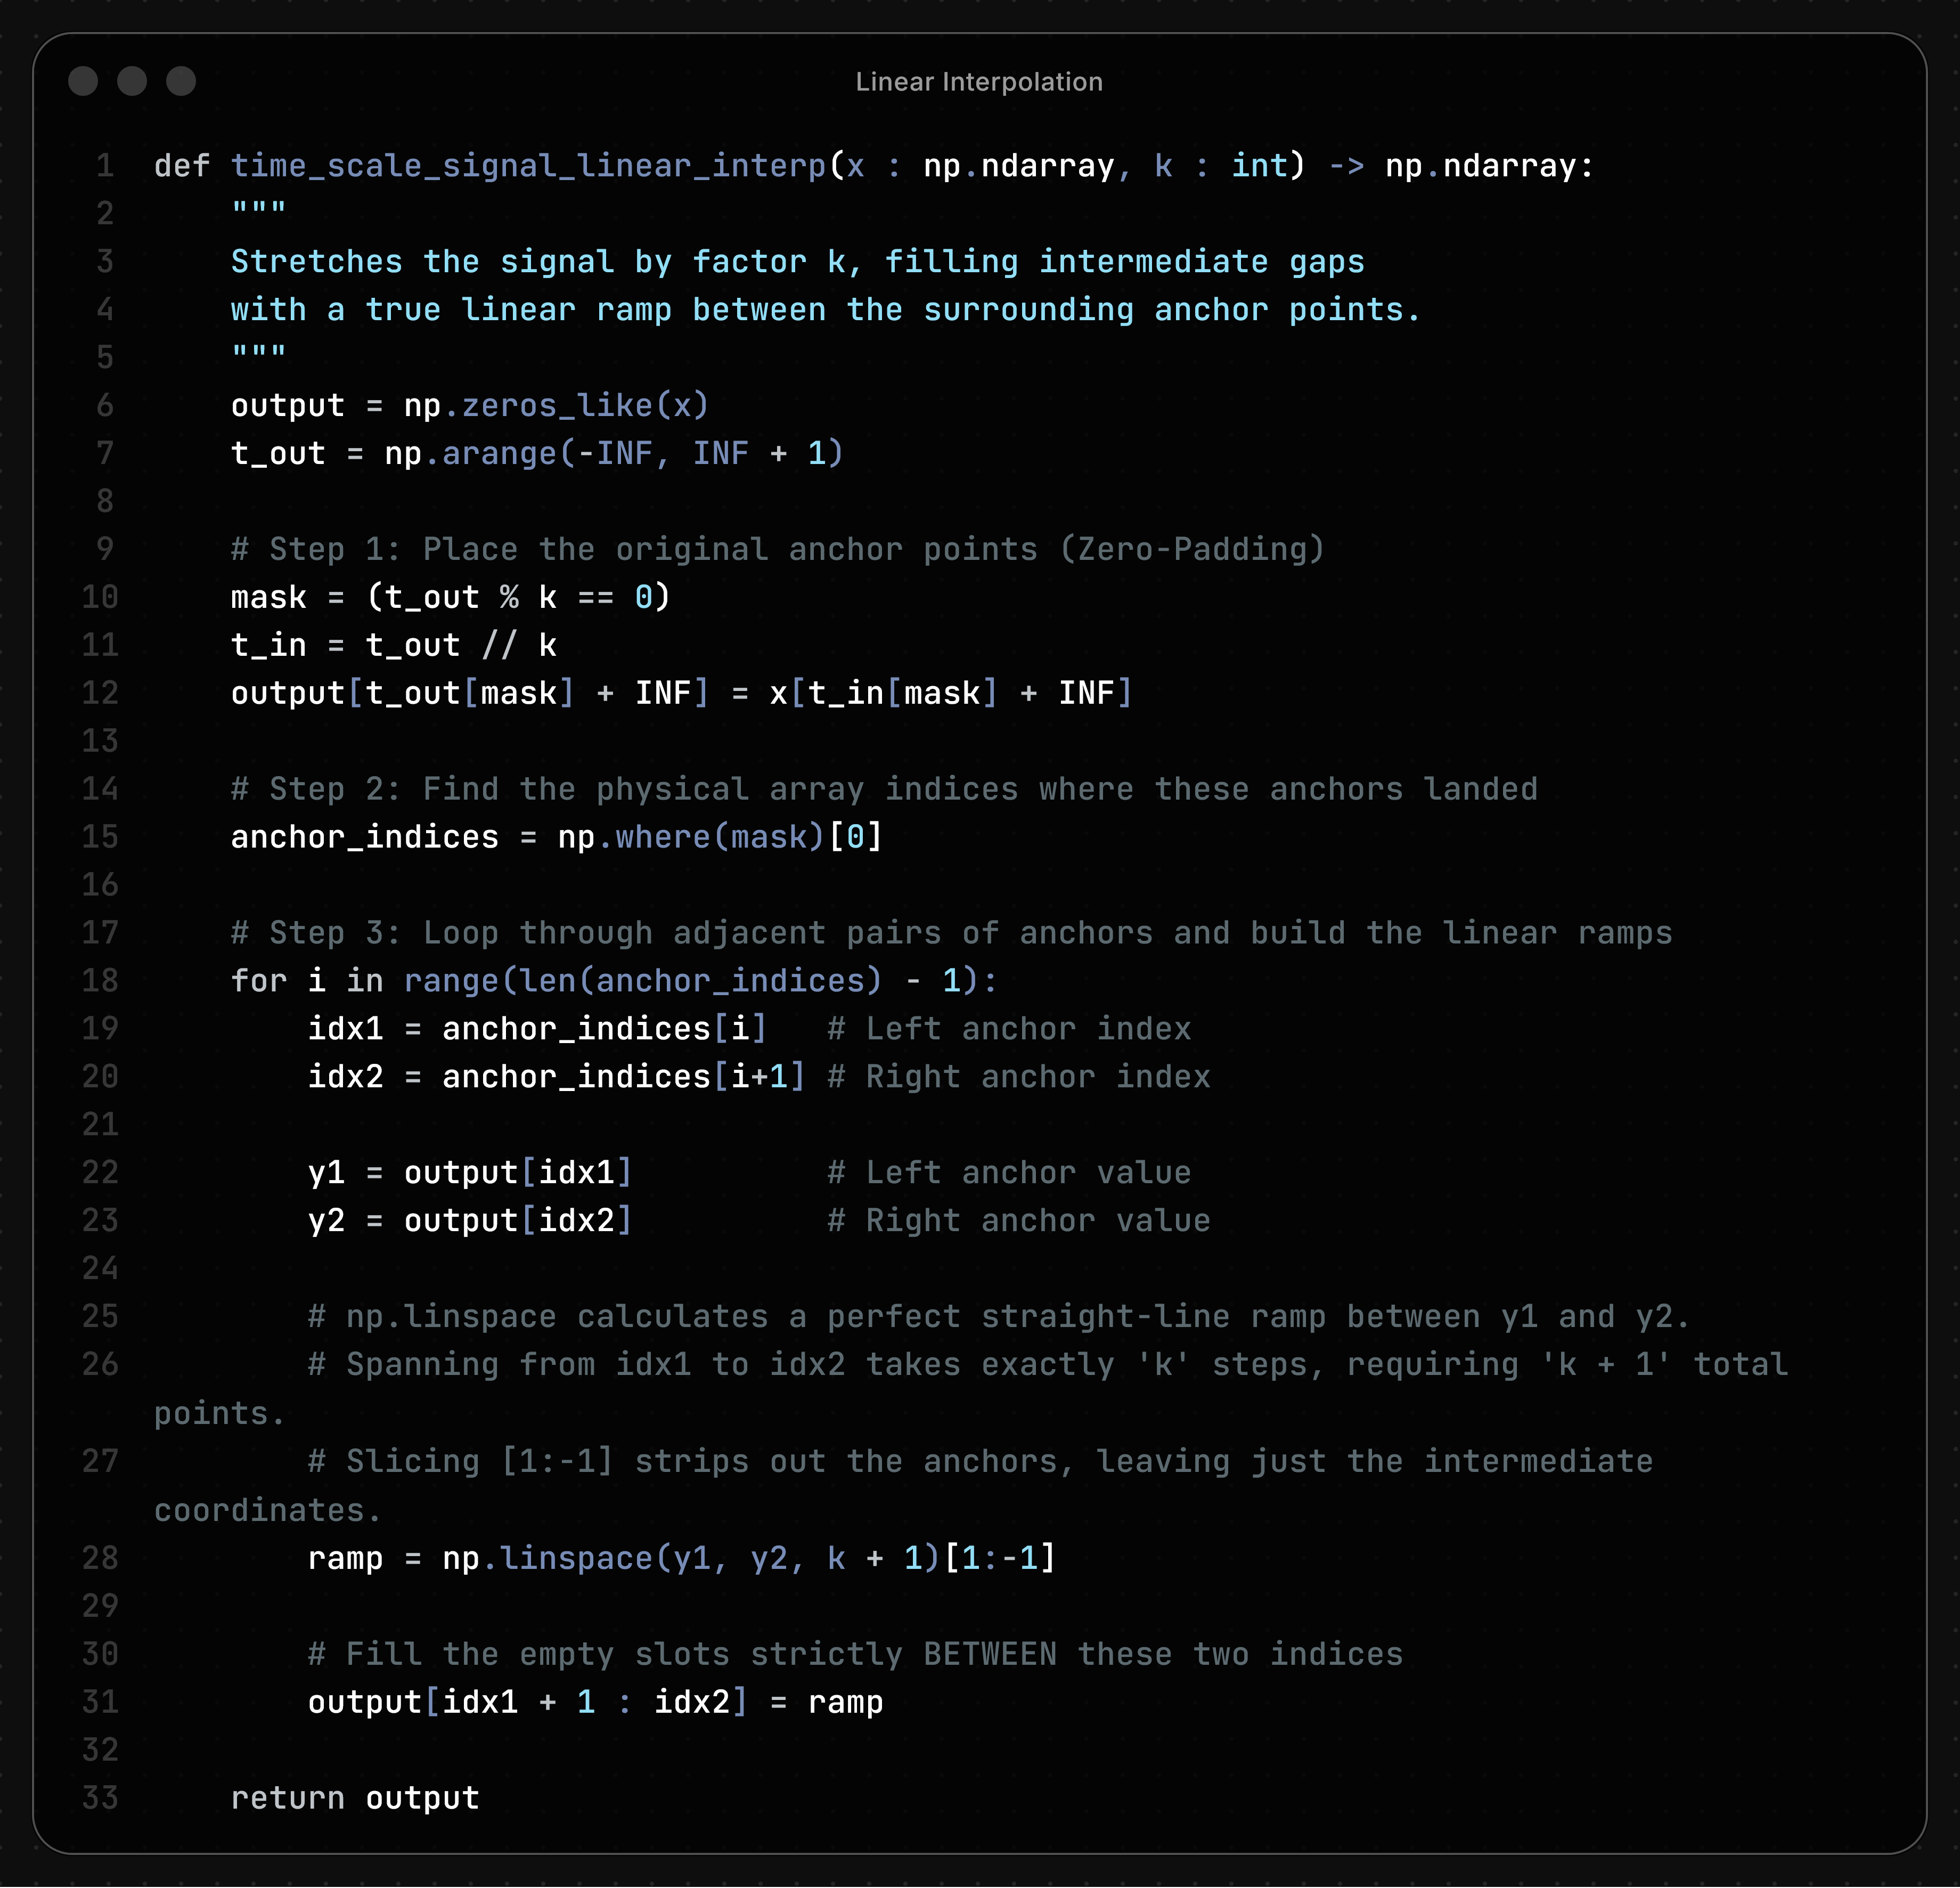
\includegraphics{li.png}} % stretched
% also valid:
% 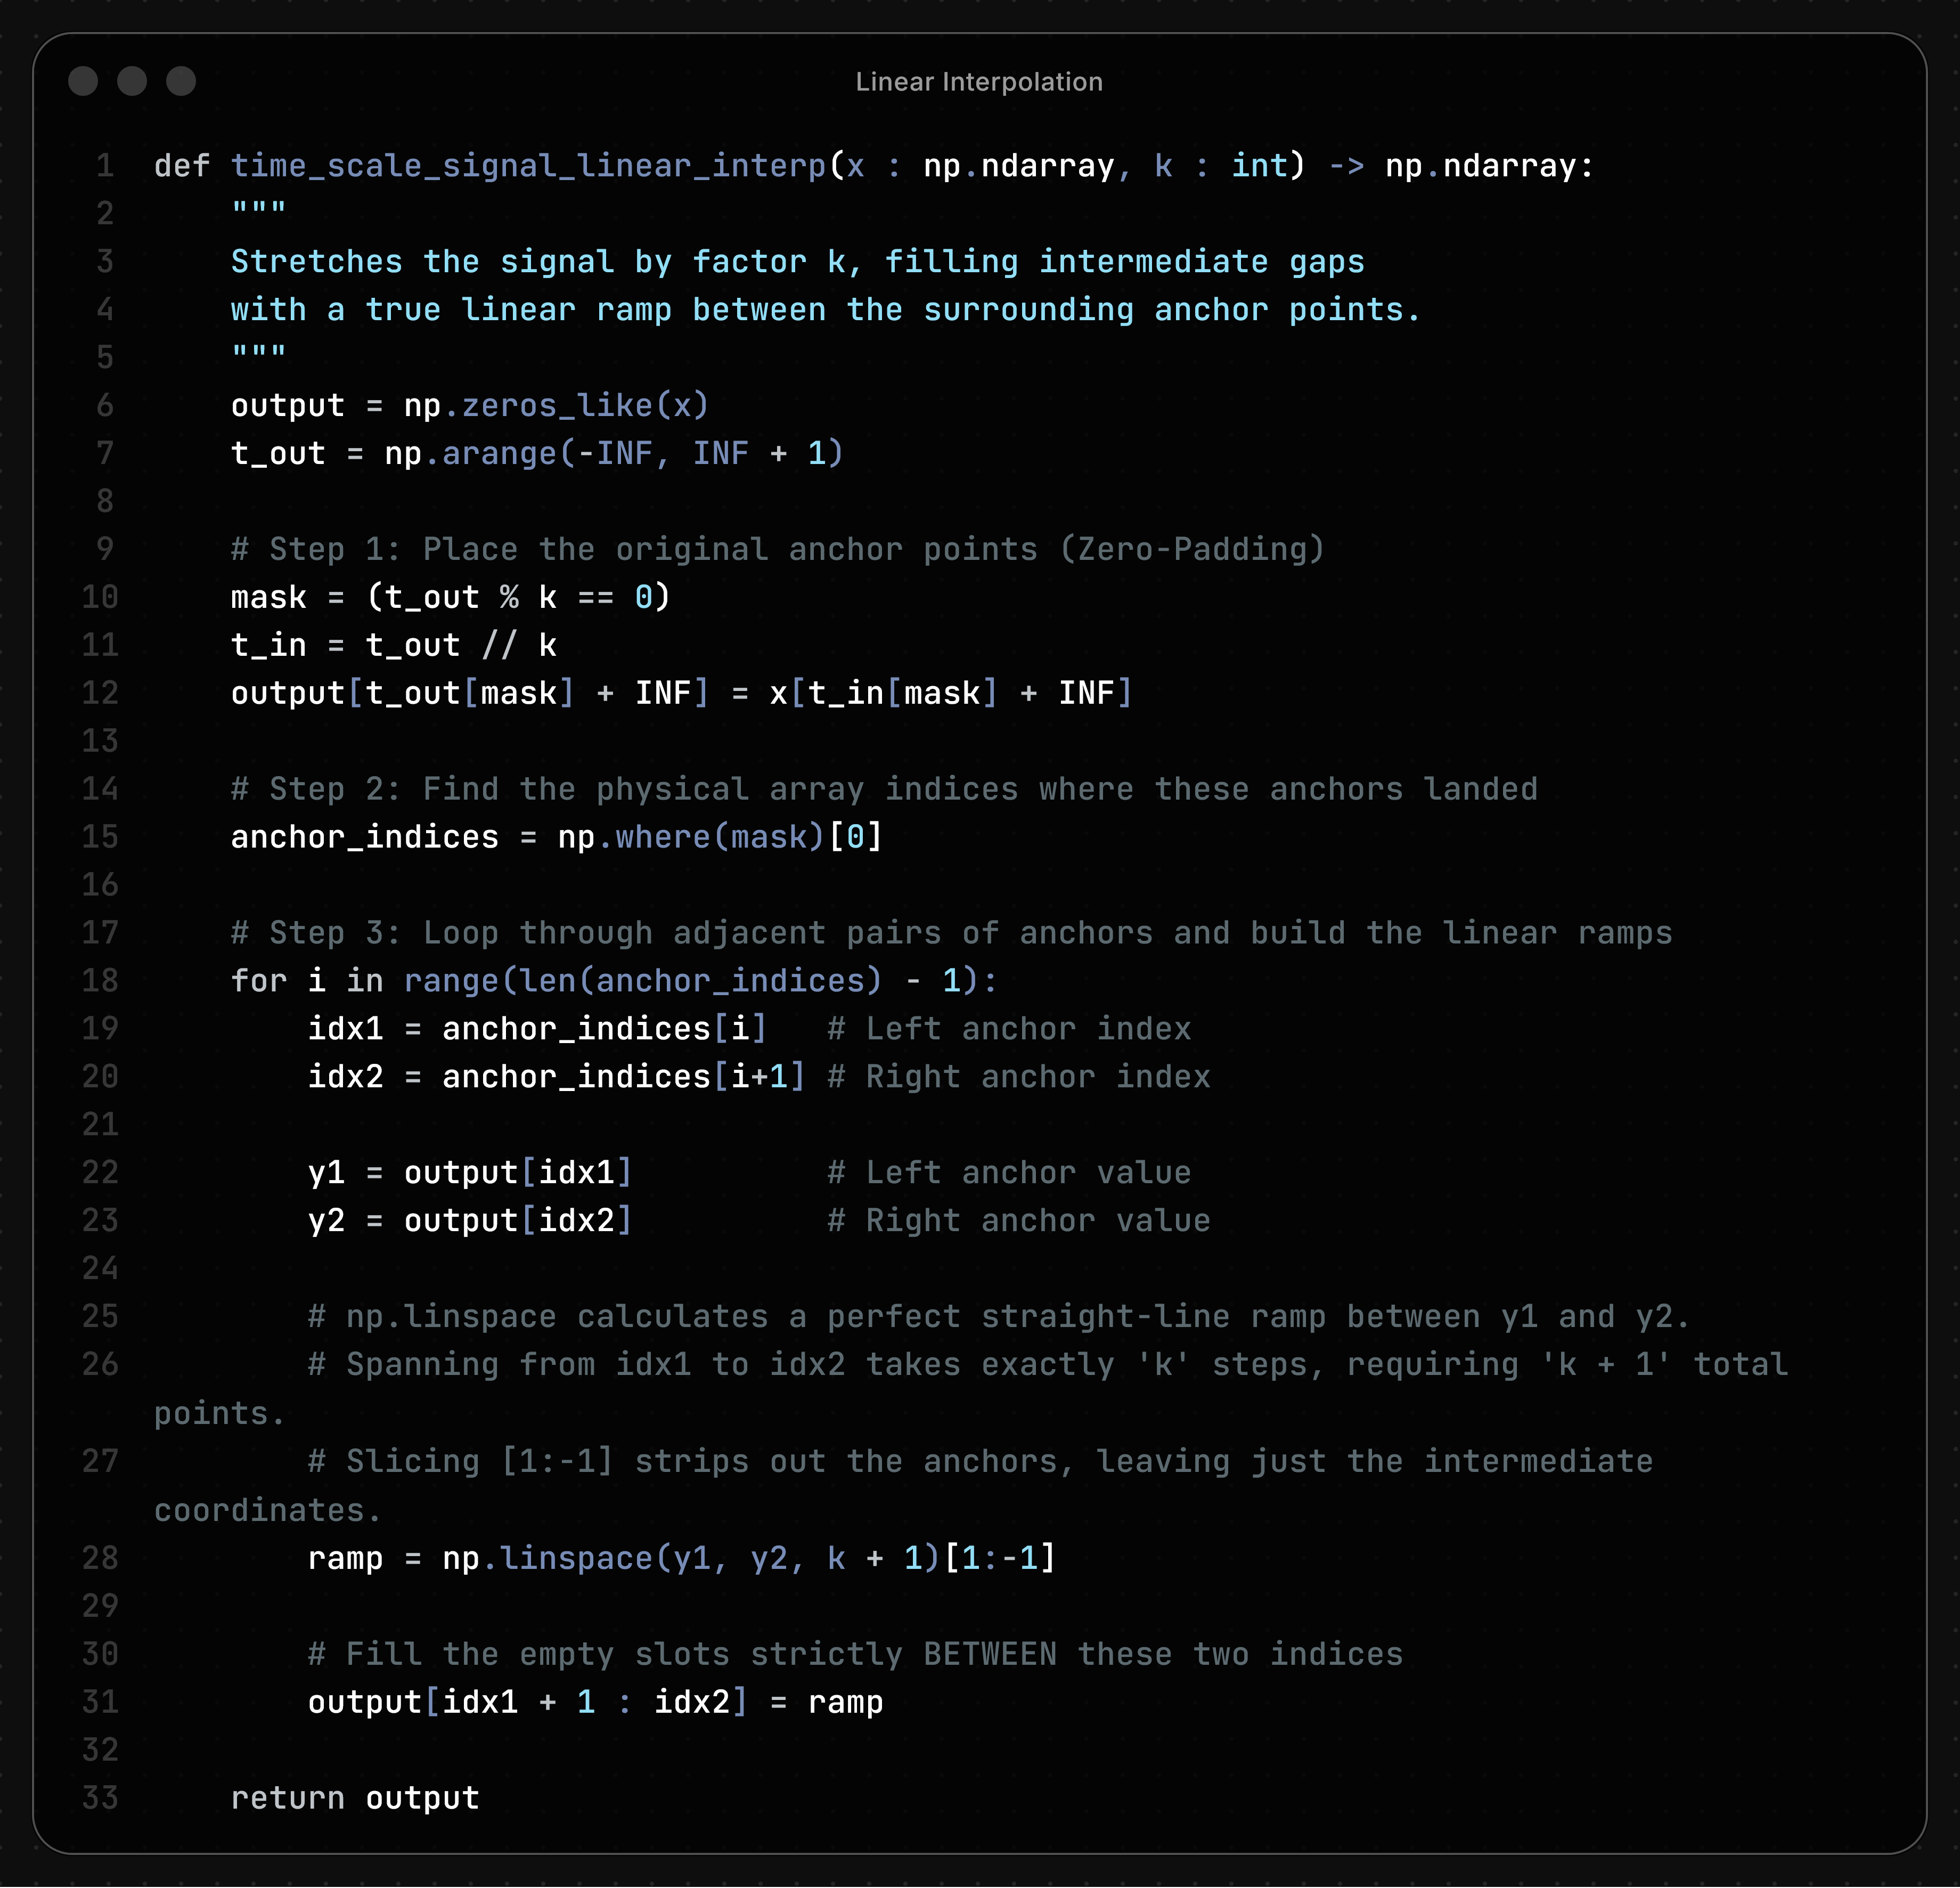
\includegraphics[scale=0.4]{li.png} % fraction of natural size


\section{Ex 09}
% \begin{figure}
    
%     \begin{minipage}[b]{0.45\textwidth}
%         \centering
%         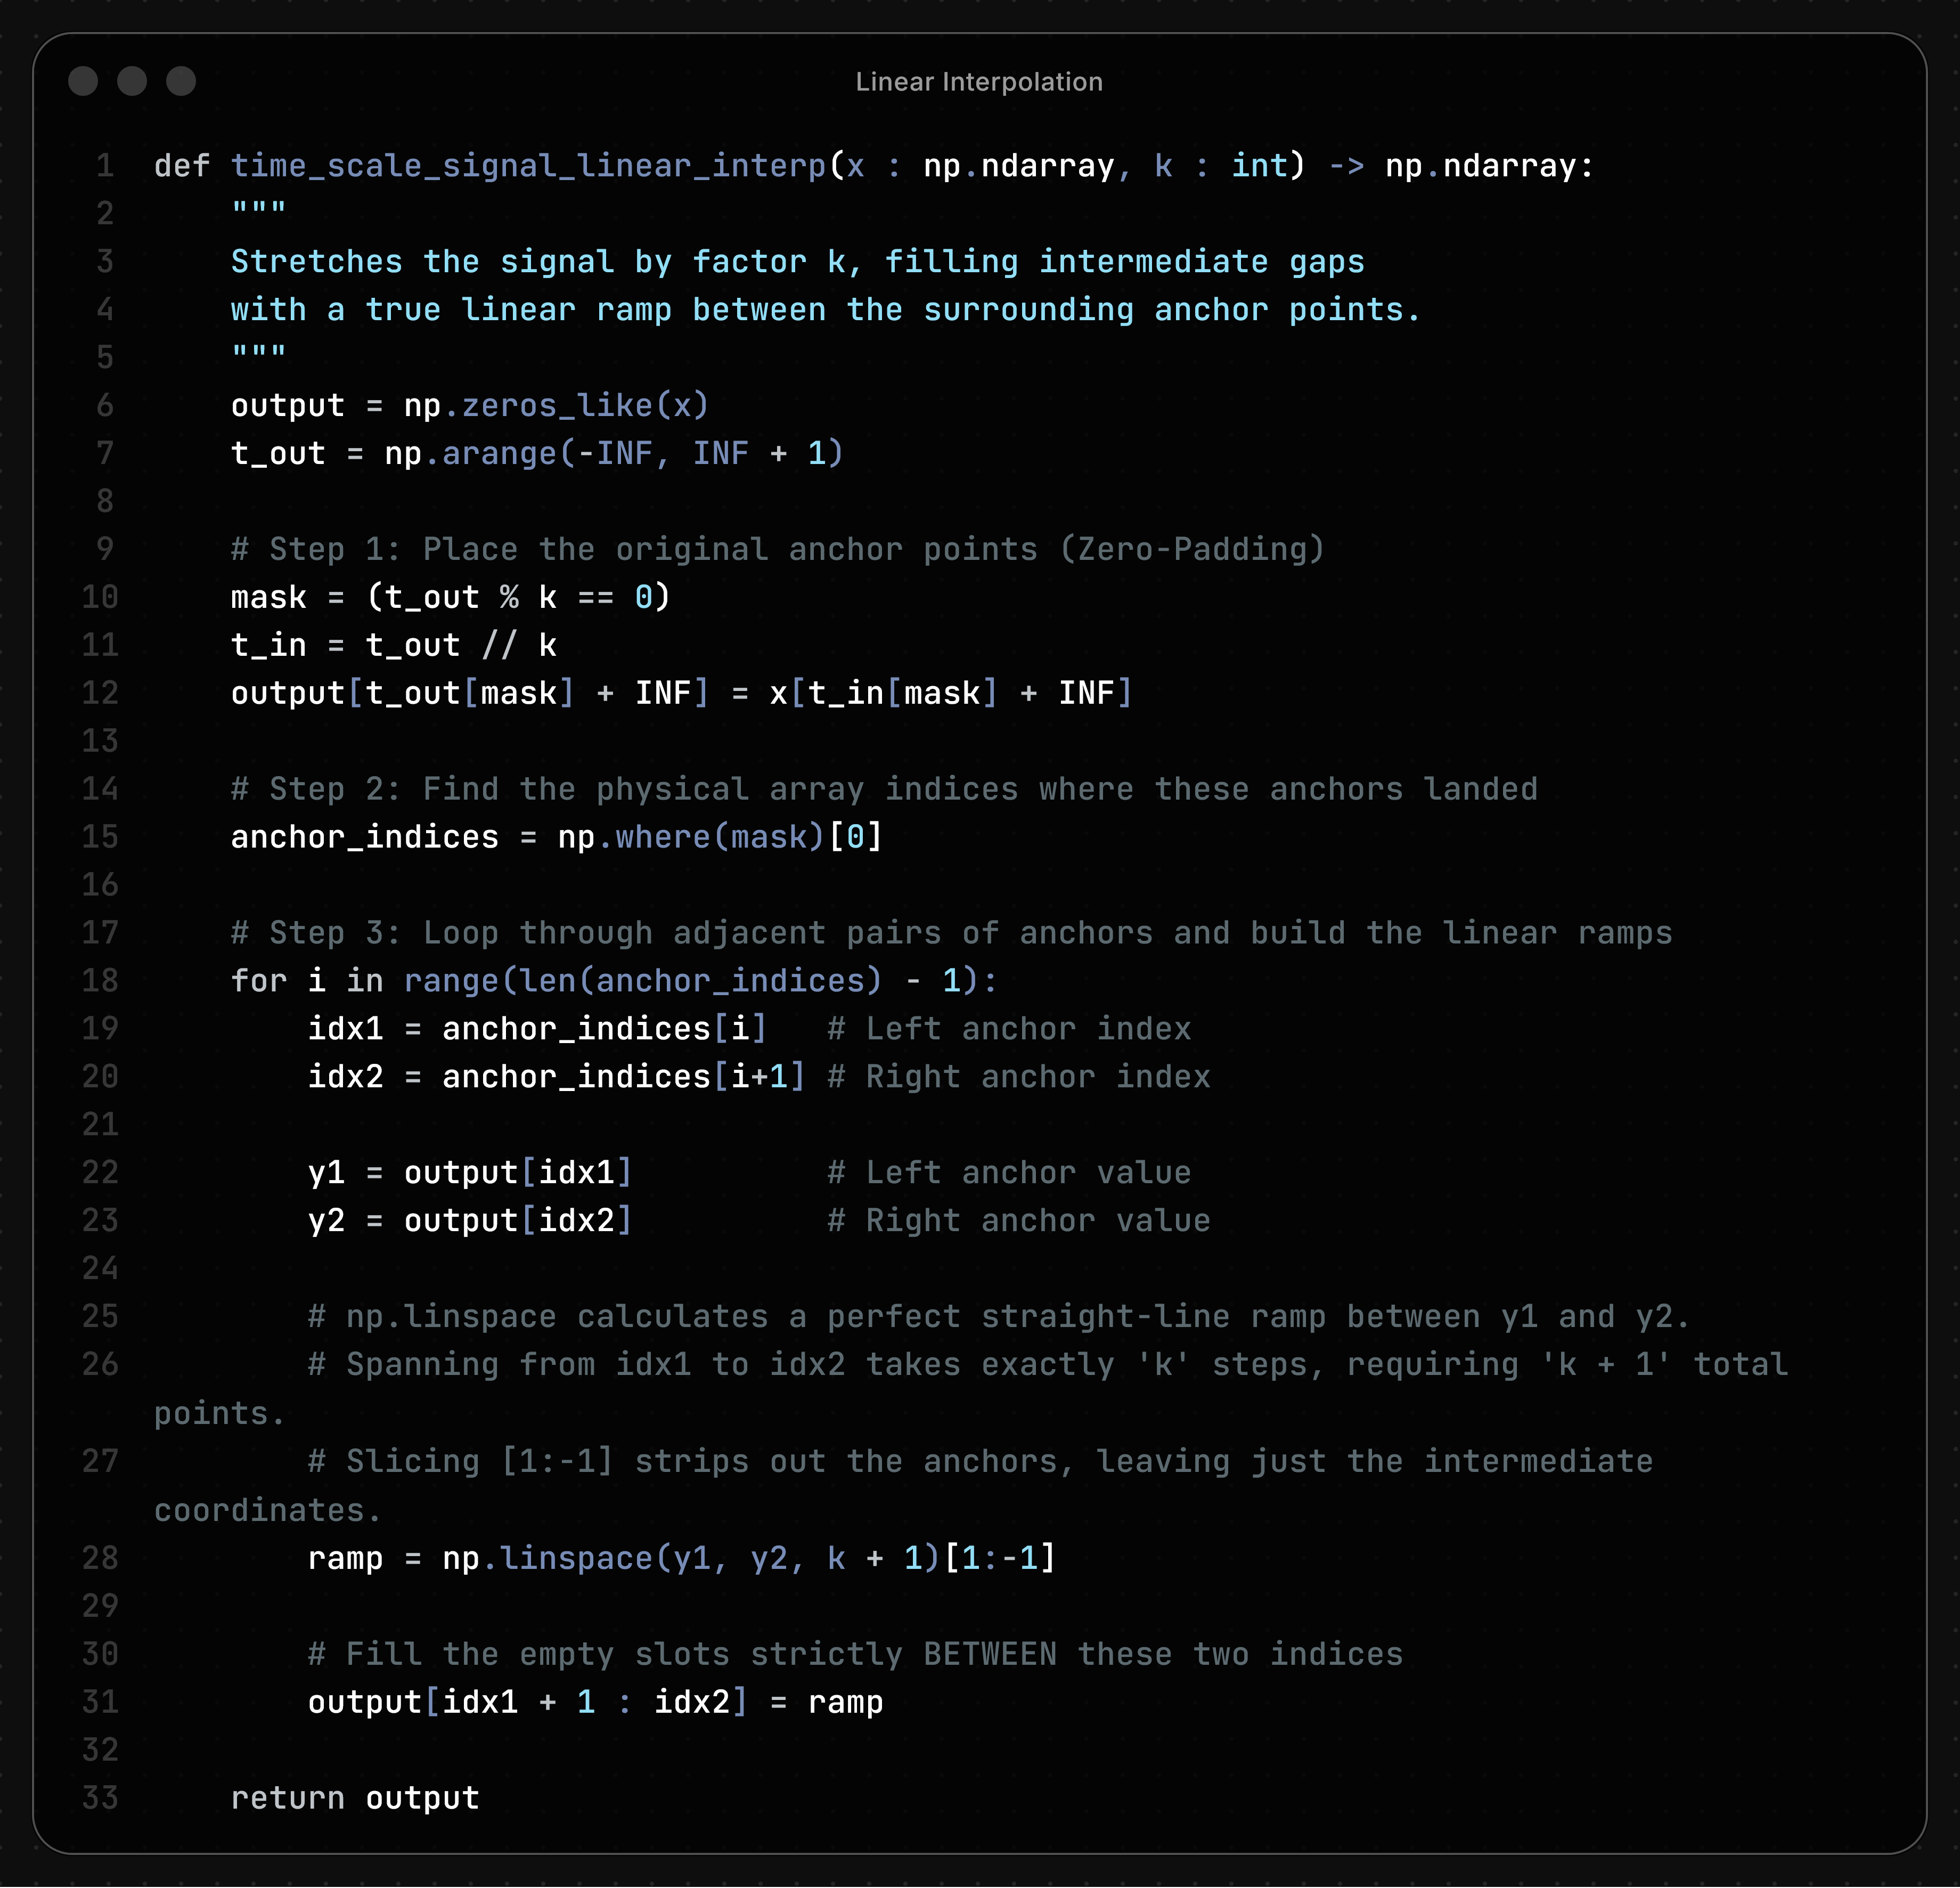
\includegraphics[width=\linewidth]{li.png}
%         \caption{kalke cookeddddddddd}
%     \end{minipage}\hfill
%     \begin{minipage}[b]{0.45\textwidth}
%         \centering
%         \captionof{Table}{Extracted Parameters}
%         \label{tab:beside}
%         \begin{tabular}{|l|c|}
%         \hline \textbf{Quantity} & \textbf{Value} \\ \hline
%         Time constant $\tau$ & $10.0$ ms \\ \hline
%         Rise time $t_r$ & $22.0$ ms \\ \hline
%         Overshoot & $4.3\%$ \\ \hline
%         \end{tabular}

%     \end{minipage}

% \end{figure}

\begin{figure}[htbp]
\centering
\begin{minipage}[b]{0.46\textwidth}
\centering
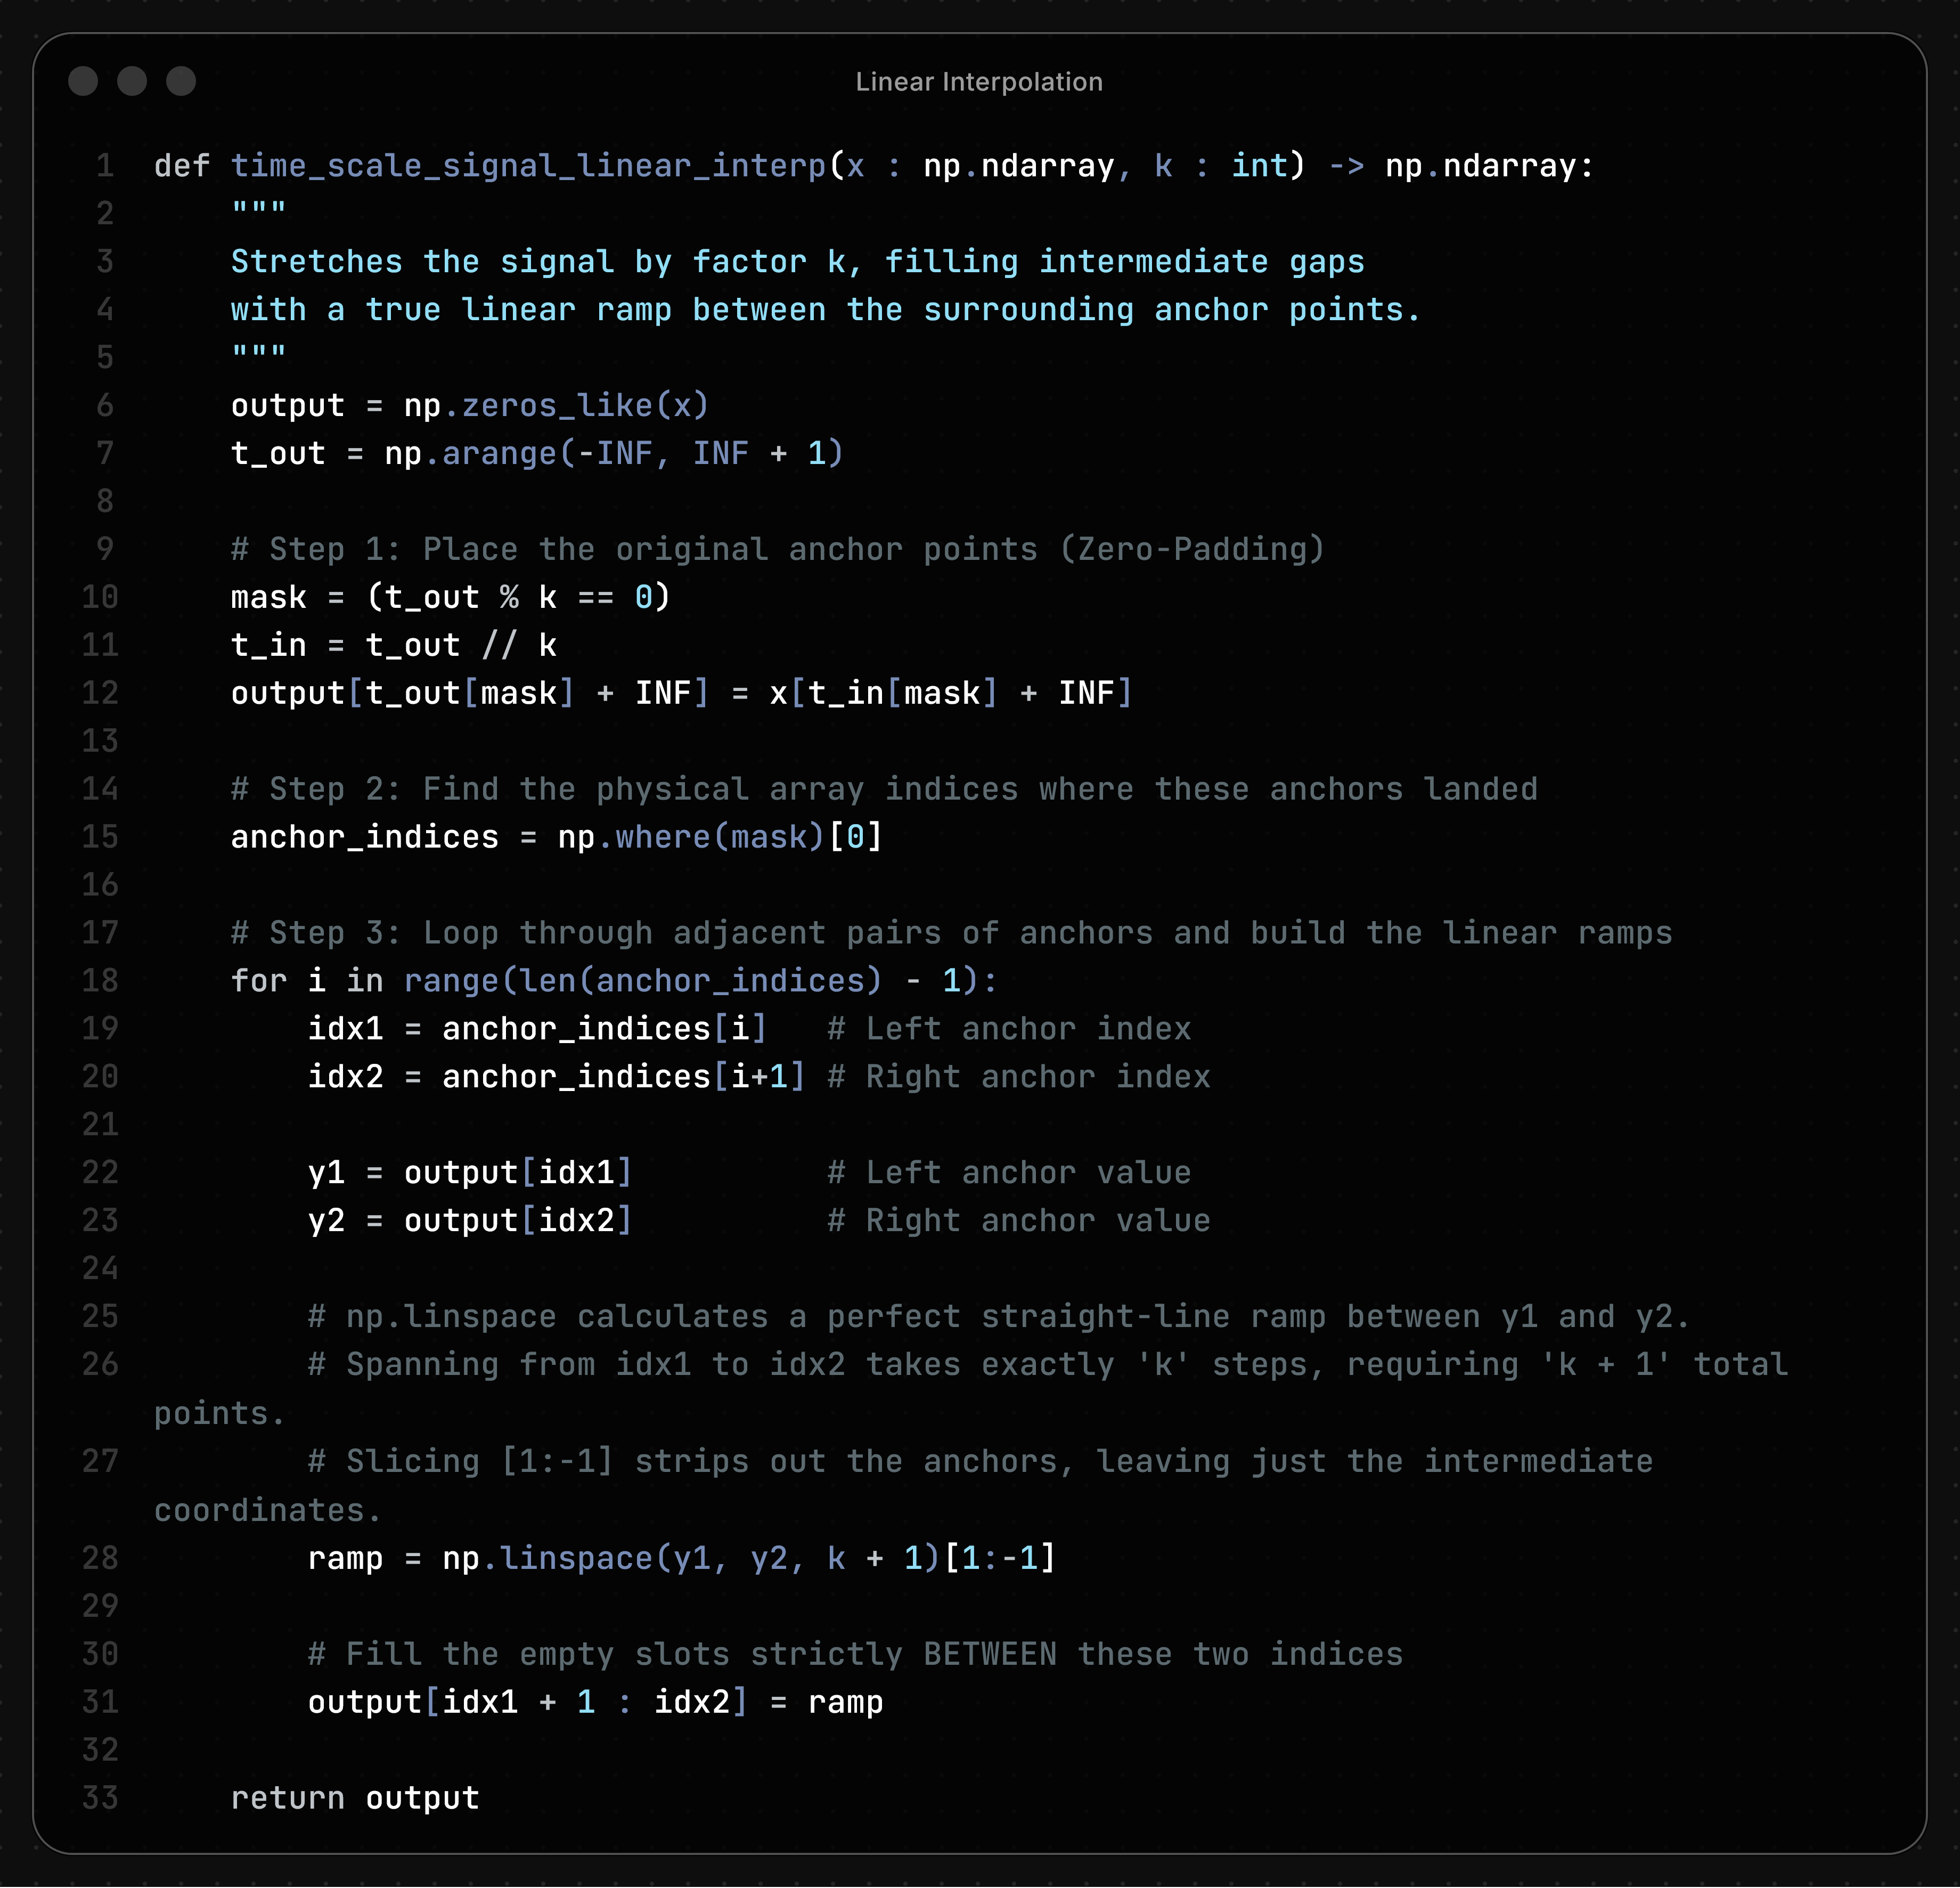
\includegraphics[width=\linewidth]{li.png}
\caption{Measured step response.}
\label{fig:beside}
\end{minipage}\hfill
\begin{minipage}[b]{0.46\textwidth}
\centering
\captionof{table}{Extracted parameters.}
\label{tab:beside}
\begin{tabular}{|l|c|}
\hline \textbf{Quantity} & \textbf{Value} \\ \hline
Time constant $\tau$ & $10.0$ ms \\ \hline
Rise time $t_r$ & $22.0$ ms \\ \hline
Overshoot & $4.3\%$ \\ \hline
\end{tabular}
\end{minipage}
\end{figure}

\end{document}